\documentclass[11pt]{report}

\usepackage[spanish]{babel} 
\usepackage[utf8]{inputenc}
\usepackage{graphicx}
\usepackage{color}
\usepackage{subfigure}
\usepackage{float}
\usepackage{capt-of}
\usepackage{sidecap}
\usepackage{caption}
\usepackage{anysize}
\usepackage{multirow}
\usepackage{graphicx}
\usepackage[table,xcdraw]{xcolor}
\usepackage[normalem]{ulem}
\useunder{\uline}{\ul}{}
\usepackage{longtable}
\usepackage{xcolor}
\usepackage[normalem]{ulem}
\usepackage{appendix}
\usepackage[colorlinks=true,plainpages=true,citecolor=blue,linkcolor=blue]{hyperref}
\usepackage{fancyhdr} 
\usepackage{listings}
\usepackage{comment}

\sidecaptionvpos{figure}{c} % Para que el texto se alinie al centro vertical
\marginsize{2cm}{2cm}{2cm}{2cm} % Izquierda, derecha, arriba, abajo
\captionsetup{labelfont={color=gray},font={color=gray}} %Cambia el color de los pies de foto/tabla
\useunder{\uline}{\ul}{}
\renewcommand{\appendixname}{Apéndices}
\renewcommand{\appendixtocname}{Apéndices}
\renewcommand{\appendixpagename}{Apéndices} 
\renewcommand{\footrulewidth}{0.4pt}
\newcommand{\sen}{\operatorname{\sen}}	% Definimos el comando \sen para el seno

\pagestyle{fancy}
\fancyhf{}
\fancyhead[L]{\footnotesize TT 2019-A104} %encabezado izquierda
\fancyhead[R]{\footnotesize IPN - ESCOM}   % dereecha
\fancyfoot[R]{\footnotesize Trabajo Terminal II}  % Pie derecha
\fancyfoot[C]{\thepage}  % centro
\fancyfoot[L]{\footnotesize Ingenier\'ia en Sistemas Computacionales}  %izquierda

\definecolor{dkgreen}{rgb}{0,0.6,0} % Definimos colores para usar en el código
\definecolor{gray}{rgb}{0.5,0.5,0.5} 

\begin{document}

\begin{center}
\newcommand{\HRule}{\rule{\linewidth}{0.5mm}}
\begin{minipage}{0.48\textwidth} \begin{flushleft}
%
\includegraphics[scale=0.09]{images/ipn.png}
\end{flushleft}\end{minipage}
\begin{minipage}{0.48\textwidth} \begin{flushright}
%
\includegraphics[scale = 0.08]{images/escom.png}
\end{flushright}\end{minipage}
\vspace*{1.5cm}
\textsc{\huge Instituto Polit\'ecnico\\ \vspace{5px} Nacional}\\[1.5cm]
\textsc{\LARGE Escuela Superior de C\'omputo}\\[1.5cm]
\begin{minipage}{0.9\textwidth} 
\begin{center}
\textsc{\LARGE Trabajo Terminal II}
\end{center}
\end{minipage}\\[0.5cm]
\vspace*{1cm}
\HRule \\[0.4cm]
{ \huge \bfseries “Sistema de realidad virtual del cuerpo humano para el estudio del sistema digestivo”
}\\[0.4cm]
\HRule \\[1.5cm]
\begin{minipage}{0.46\textwidth}
\begin{flushleft} \large
\emph{Autor:}\\	
Almendarez Perdomo Rodrigo\\
\end{flushleft}
\end{minipage}
\begin{minipage}{0.52\textwidth}		
\vspace{-0.6cm}
\begin{flushright} \large
\emph{Directores:} \\
M. en Ing. Moscoso Malagón Yosafat\\
M. en C. Saucedo Delgado Rafael Norman
\end{flushright}
\end{minipage}
\vspace*{1cm}
\vspace{1cm}	
\emph{Para obtener el t\'itulo de }\\
\vspace{1cm}	
{\textbf{\Large Ing. en Sistemas Computacionales}	}\\
\vspace{1cm}
\begin{center}
{\large \today}
\end{center}											  						

\begin{abstract}												
\begin{minipage}{0.48\textwidth} \begin{flushleft}

\includegraphics[scale = 0.09]{images/ipn}
\end{flushleft}\end{minipage}
\begin{minipage}{0.48\textwidth} \begin{flushright}

\includegraphics[scale = 0.08]{images/escom}
\end{flushright}\end{minipage}

El presente proyecto consiste en desarrollar un software que está enfocado a la enseñanza, aprendizaje y demostración del cuerpo humano mediante Realidad Virtual (R.V.), el mismo que puede ser usado en la Escuela Superior de Medicina (E.S.M.) y Escuela Nacional de Medicina y Homeopatía (E.N.M. y H.) en las áreas de Morfología y Anatomía como soporte para la enseñanza de las áreas antes mencionadas. 
\\
De esta manera se espera aumentar el número de herramientas que poseen los estudiantes de medicina y reforzar el aprendizaje del alumnado con tecnología actual, escalable, con mayor disponibilidad y facilidad de uso, en contraste con el uso de cadáveres humanos.
\\[4cm]
\textbf{Palabras clave} - Animación por Computadora, Gráficos por Computadora, Realidad Virtual, Estudio Multimedia
\\[2cm]
\textbf{Presenta:}
\\[0.5cm]
Almendarez Perdomo Rodrigo
\\[2cm]
\textbf{Directores}
\\[0.5cm]
M. en Ing. Moscoso Malagón Yosafat
\\
M. en C. Saucedo Delgado Rafael Norman
\\
\end{abstract}							

\section*{Advertencia}
\textit{“Este documento contiene información desarrollada por la Escuela Superior de Cómputo del Instituto Politécnico Nacional, a partir de datos y documentos con derecho de propiedad y, por lo tanto, su uso quedará restringido a las aplicaciones que explícitamente se convengan.”
\\
La aplicación no convenida exime a la escuela su responsabilidad técnica y da lugar a las consecuencias legales que para tal efecto se determinen. 
\\
Información adicional sobre este reporte técnico podrá obtenerse en: 
\\
La Subdirección Académica de la Escuela Superior de Cómputo del Instituto Politécnico Nacional, situada en Av. Juan de Dios Bátiz s/n Teléfono: 57296000, extensión 52000.}

\section*{Agradecimientos}
\vspace*{\fill}
En primer lugar quiero agradecer a mis directores, M. en Ing. Moscoso Malagón Yosafat y el M. en C. Saucedo Delgado Rafael Norman, quienes con sus conocimientos y apoyo me guiaron a través de cada una de las etapas de este proyecto para alcanzar los resultados que buscaba, después de todo el  desarrollo de un Trabajo Terminal es el pináculo de  la formación de un alumno en la carrera de Ingeniería en Sistemas Computacionales, el cual requiere de mucha dedicación y conocimientos para llegar a su desarrollo exitoso.
Especialmente quiero agradecer al profesor Alfredo Rangel Guzmán por sus enseñanzas sobre la vida y el actuar del mundo actual, y el recibir su apoyo incondicional.
También quiero agradecer a la Escuela Superior de Cómputo por brindarme todos los recursos, herramientas y conocimientos que fueron necesarios para llevar a cabo el proceso de investigación y desarrollo del Trabajo Terminal. No hubiese podido arribar a estos resultados de no haber sido por su incondicional ayuda.
Por último, quiero agradecer a todos mis compañeros y amigos, principalmente a los que me han acompañado desde el inicio de mi carrera y a mi familia y pareja, por apoyarme aún cuando mis ánimos decaían. En especial, quiero hacer mención de mis padres, que siempre estuvieron ahí para darme palabras de apoyo y un abrazo reconfortante para renovar energías y continuar trabajando para finalizar este camino.
Muchas gracias a todos.
\vspace*{\fill}
\paragraph{Rodrigo Almendarez Perdomo}


\tableofcontents

\chapter{Presentación del problema}

\section{Contexto y motivación}
La Escuela Superior de Medicina del Instituto Politécnico Nacional tiene su antecedente en la Carrera de Medicina Rural creada en 1938, desde entonces ha tenido varias adaptaciones y recintos, siendo el año de 1945 en el que fue creada por decreto oficial la Escuela Superior de Medicina Rural y finalmente en 1957 tuvo sus instalaciones propias, ya que en años previos había tenido que operar en instalaciones de otras Unidades Académicas del Instituto. En 1965 fue suprimido de su nombre el calificativo Rural y en lo sucesivo fue su nombre tal como actualmente se le conoce Escuela Superior de Medicina (ESM) y que es la Unidad Académica del IPN encargada de formar médicos cirujanos. (Fuente de referencia https://www.esm.ipn.mx/conocenos/mision.html)\\
Para cualquier estudiante de Medicina es fundamental y requisito conocer e interactuar con los sistemas del cuerpo humano, por ejemplo,  para la enseñanza de la anatomía y de morfología es indispensable el uso de cuerpos para su disección y análisis.\\
Actualmente en la Escuela Superior de Medicina y Homeopatía y la Escuela Superior de Medicina, utilizan principalmente medios impresos tradicionales y uso de cuerpos como principales materiales y recursos para  la enseñanza y aprendizaje.\\
El uso de cuerpos para su disección en la ESM tiene sus particularidades, por ejemplo, los costos inherentes al mantenimiento de los cuerpos en las instalaciones, frecuentemente se enfrenta el problema de que los cuerpos no son suficientes para la cantidad de alumnos en determinadas clases, algunas veces se deben de compartir los cuerpos con otras instituciones y cuando el cuerpo ya no puede seguir siendo utilizado se debe realizar su inhumación.\\
Hay además algunas problemáticas que ha enfrentado la ESM, como el mantenimiento óptimo de las instalaciones, particularmente relacionado a lo que se ha mencionado del uso de los cuerpos para exploración, del anfiteatro. Sobre esto a raíz del sismo de septiembre de 2017, se dañaron varios edificios así como el anfiteatro, en el caso de este último quedando inutilizable durante casi seis meses, lo cual obligó  a los docentes a reformular sus clases de morfología y anatomía usando presentaciones de diapositivas y algunos videos. Este tipo de problemas incide directamente en la parte práctica que debe realizar el estudiante de medicina, en este caso en particular, en el semestre siguiente el rendimiento de los estudiantes se vio disminuido a causa de la falta de práctica física con los cuerpos.\\
Teniendo conocimiento de este tipo de problemas y con la intención de crear una herramienta de software que utilizará la Realidad Virtual, en septiembre de 2018 se entrevistó al Dr. Rios Macias Jefe del Área de Morfología de la Escuela Superior de Medicina (ESM) del Instituto Politécnico Nacional (IPN) y comentó que “los medios que se utilizan para el estudio del cuerpo humano principalmente son impresos tradicionales, así como el uso de cuerpos para su disección y análisis posterior”. Derivado de las entrevistas realizadas, se sabe que, son muchos los subsistemas del cuerpo humano y que la creación de materiales distintos a los libros y materiales impresos, puede ser un área de oportunidad que ofrezca a los estudiantes una alternativa extra para explorar y reforzar sus conocimientos, aunque hasta ahora no es posible reemplazar la interacción de los estudiantes con el cuerpo humano real.1.2 Propuesta de Solución
Considerando que son muchos los subsistemas que integran el cuerpo humano, se ha elegido el sistema digestivo. Por lo tanto, este documento presenta un prototipo de sistema de realidad virtual del sistema digestivo del cuerpo humano que permite interactuar con modelos tridimensionales de los órganos que lo conforman. La intención podría ser sentar un precedente de un sistema de apoyo al aprendizaje que favorezca la interacción práctica [ 1 ] de los estudiantes de la ESM.\\

\section{Objetivos del Sistema}
Analizar, diseñar, desarrollar y probar un prototipo de sistema que utiliza la tecnología de Realidad Virtual, para ofrecer una experiencia orientada al estudio 
de la anatomía y morfología del cuerpo humano, específicamente del sistema digestivo.\\
\subsection{Objetivos Específicos}
\begin{itemize}
	\item Utilizar como insumo para la elaboración de los modelos, las referencias documentales y confiables que proporcionan los expertos del área de morfología de la ESM del IPN sobre el sistema digestivo.
	\item Elaboración de modelos en tres dimensiones del sistema digestivo humano
	\begin{enumerate}
		\item Glándulas Salivales
		\item Cavidad Oral
		\item Faringe
		\item Esófago
		\item Estómago
		\item Intestino Delgado
		\begin{enumerate}
		  \item Hígado
		  \item Páncreas
		  \item Vesícula Biliar
		\end{enumerate}
		\item Intestino Grueso y Ano  
	  \end{enumerate}
	\item Diseñar y desarrollar
	\item Probar los componentes de software del sistema y realizar su interacción con los elementos de hardware que propiamente proporcionan el entorno de  Realidad Virtual.	
\end{itemize}

\section{Revisión del Estado del Arte}
A continuación se muestran algunos de trabajos académicos desarrollados en México y fueron comparados con el trabajo planeado. 
Como comparativa y de forma ilustrativa del sector académico.\\
\newline
\begin{enumerate}
\item TT No. 2014-A058 “Sistema para la orientación de los efectos sobre la espalda humana en pacientes con sobrepeso”\cite{tt1}
\item TT No. 2012-B055 “Laboratorio Virtual del cuerpo humano 3D con asistente de ayuda en línea para el nivel superior bajo el paradigma de Educación Basada en Web con 
tecnologías de Web Semántica”\cite{tt2}
\item TT No. 2014-B035 “Simulación en Tercera Dimensión del Sistema Circulatorio de los Cánidos para el uso Educativo”\cite{tt3}
\item TT No. 2014-B039 “Simulación de una Línea del Metro con Realidad Virtual”\cite{tt4}
\item Tesis que para optar por el grado de Maestro en Ciencia e Ingeniería de la Computación, Sistema de seguimiento de movimiento de las extremidades superiores basado 
en sensores inerciales para rehabilitación en realidad virtual.\cite{mastersthesis1}
\item Adecuación educativa de la realidad virtual como herramienta didáctica para el proceso enseñanza-aprendizaje / tesis que para obtener el título de Licenciado en 
Pedagogía, presenta Maria de la O García Noriega; asesor Lucina Moreno Valle Suárez.\cite{te1}
\end{enumerate}
Así mismo se ha encontrado software propietario desarrollado por empresas privadas los cuales son los siguientes.\\
\begin{itemize}
\item The Body VR: Anatomy Viewer es la única herramienta de visualización de Realidad Virtual disponible en el mercado que se basa en datos médicos específicos del 
paciente (por ejemplo, MRI, CT, PET) y cumple con los estándares DICOM. Proporciona simulaciones de R.V. anatómicas en tiempo real para visualizar diagnósticos médicos, 
ilustrar el impacto de los procedimientos y tratamientos, y crear una toma de decisiones más educada.\
\begin{figure}[H]
	\begin{center}
 		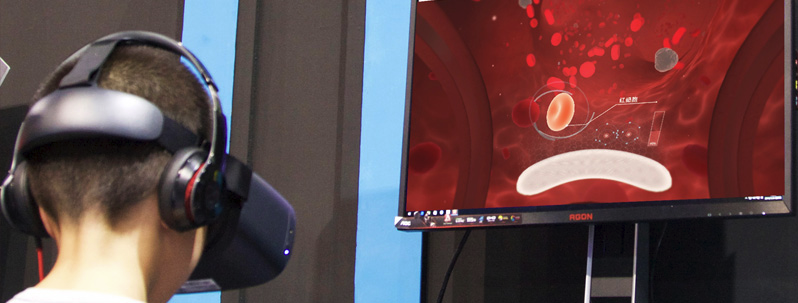
\includegraphics[width = 0.5\textwidth]{source/images/image9.png}
 		\captionof{figure}{\label{fig:ea1}Software “The Body VR” en uso.}
	\end{center} 
\end{figure}
\item Anatomyou VR: Estructuras anatómicas fotorrealistas, modeladas en colaboración con RenderArea, validadas por expertos clínicos y certificadas por personal capacitado 
en  Tecnologías Médicas de la Universidad de Las Palmas de Gran Canaria.
\begin{figure}[H]
	\begin{center}
 		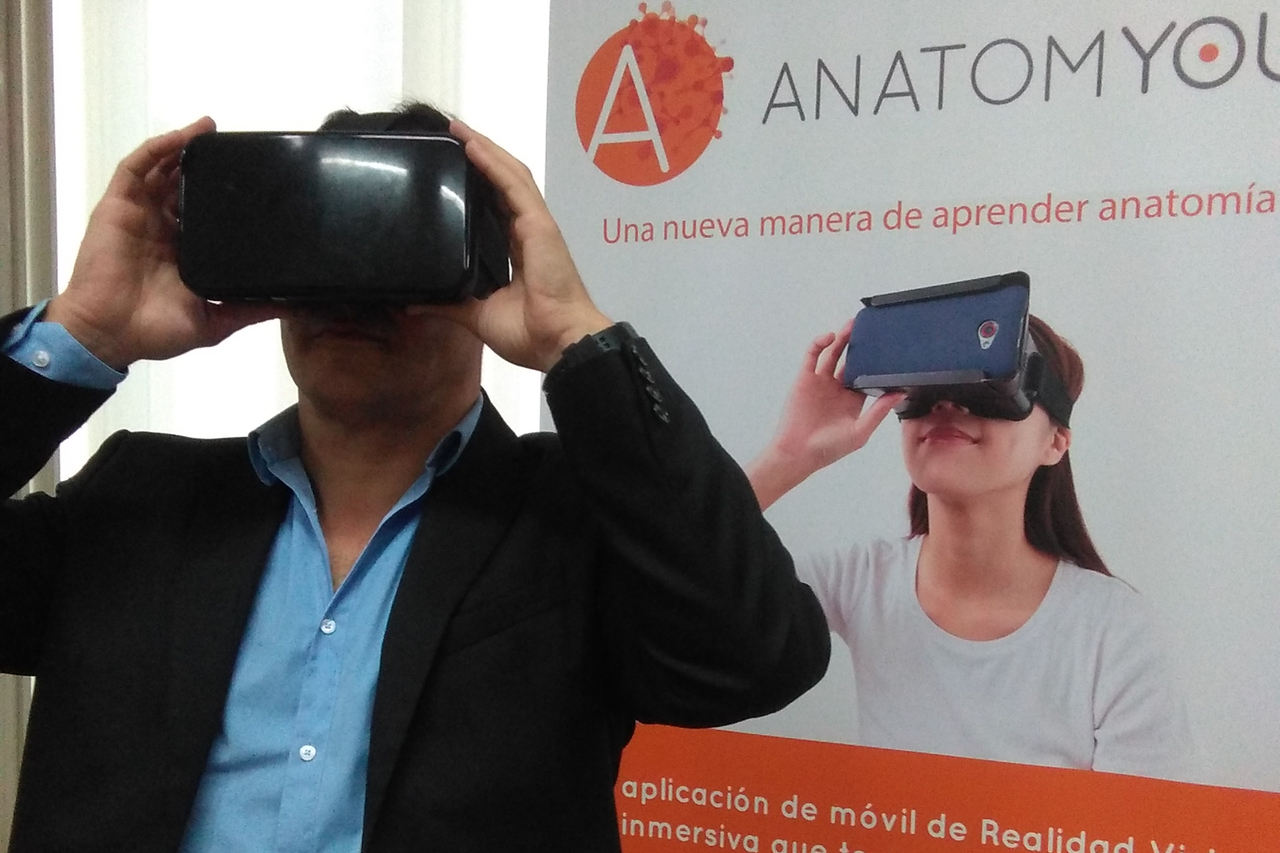
\includegraphics[width = 0.5\textwidth]{source/images/image59.png}
 		\captionof{figure}{\label{fig:ea2}Pancarta promocional de “Anatomyou VR}
	\end{center} 
\end{figure}
\item Biodigital Anatomy: El cuerpo tridimensional más completo, científicamente preciso e interactivo jamás ensamblado. Anatomía masculina y femenina, en los detalles 
básicos (gratuitos) y profesionales. Cada sistema está completamente segmentado, etiquetado y direccionable para una fácil configuración que satisfaga cualquier necesidad educativa.
\begin{figure}[H]
	\begin{center}
 		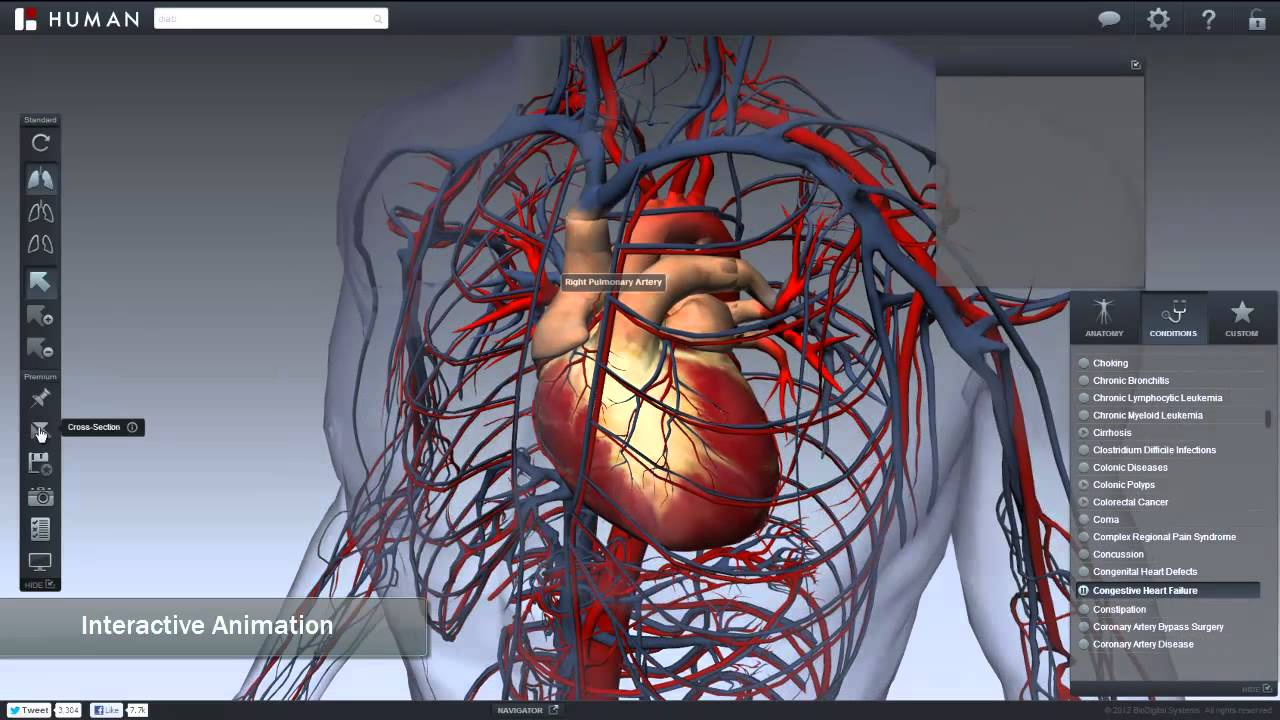
\includegraphics[width = 0.5\textwidth]{source/images/image18.png}
 		\captionof{figure}{\label{fig:ea3}Interfaz del software de Biodigital Anatomy}
	\end{center} 
\end{figure}
\item 3D Organon VR Anatom: 3D Organon es un completo atlas anatómico que presenta los 15 sistemas del cuerpo humano. Incluye más de 4,000 estructuras y órganos anatómicos 
realistas y más de 160 correlaciones clínicas encontradas por sistema del cuerpo.
\begin{figure}[H]
	\begin{center}
 		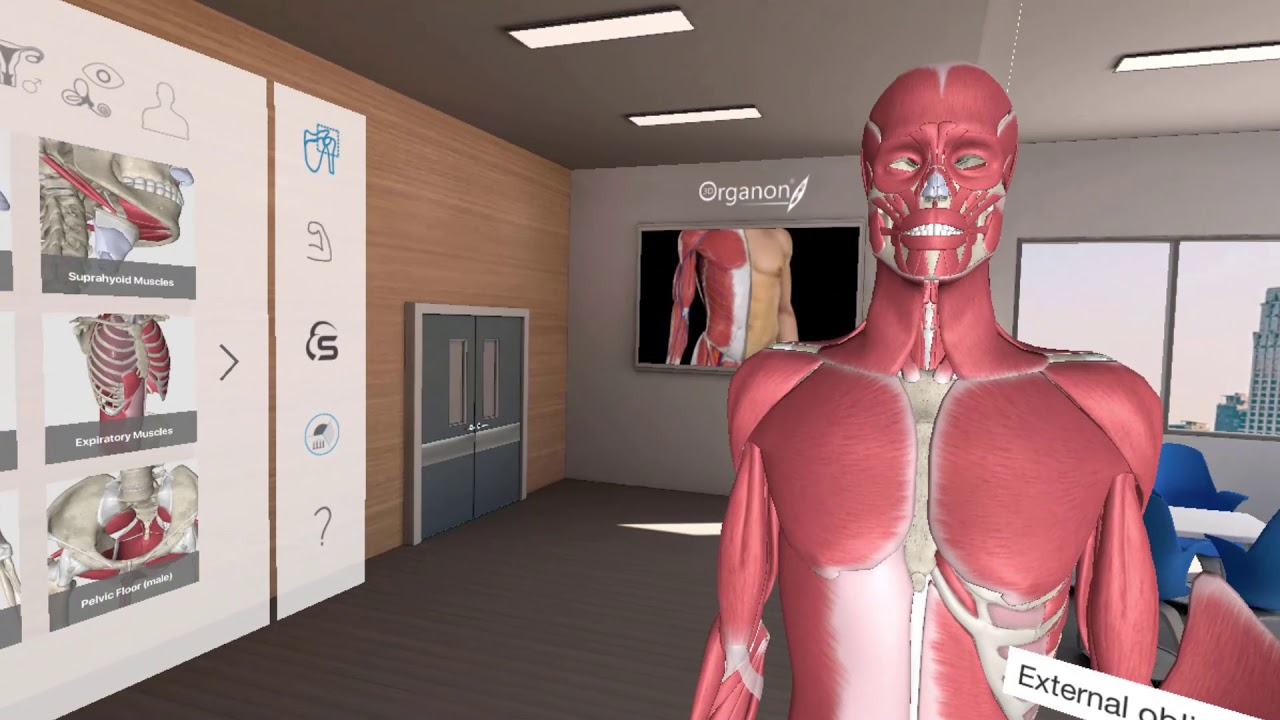
\includegraphics[width = 0.5\textwidth]{source/images/image5.png}
 		\captionof{figure}{\label{fig:ea4}Interfaz del software de 3D organon VR Anatom}
	\end{center} 
\end{figure}
\end{itemize}

\section{Organización de capítulos}
%Modificar conforme nueva organizacion
Este documento es el reporte técnico final del trabajo terminal titulado “Sistema de Realidad Virtual del Cuerpo Humano para el Estudio del Sistema Digestivo” con número de registro TT: 2019-A104.

En el \textbf{Capítulo} p se habla del problema identificado, por qué se considera como tal y cómo es que se ayudó a resolver el problema planteado mediante la ingeniería en sistemas computacionales. También se menciona que se obtiene al concluir con este trabajo terminal, tales como el prototipo del sistema.\\

En el \textbf{Capítulo II Marco Conceptual} se mostrarán todos los diagramas y documentos generados al analizar y generar un diseño del sistema que se estará desarrollando. Aquí se encuentra la arquitectura general del sistema, y los modelos gráficos de apoyo presentados en el Análisis Estructurado Moderno.\\

En el \textbf{Capítulo III Soluci\'on Propuesta} se describe el trabajo generado en el desarrollo del documento hasta el mes de mayo de 2020 para TT2.\\

En el \textbf{Capítulo IV Pruebas Experimentales} se muestran pruebas hechas sobre las implementaciones del sistema siguiendo un guión para la prueba.\\
 
En el \textbf{Capítulo V Conclusiónes y Trabajo a Futuro} se muestran los resultados obtenidos y experiencias para mejorar el proceso, así como la vertiente para continuar con el trabajo y las conclusiones del integrante.\\

Finalmente, se encuentran las Referencias de todos los recursos empleados para dar soporte y estructura a este Trabajo Terminal, y en los apéndices se anexan elementos extra que dan información más detallada sobre lo que aquí fue realizado.\\
La estiLa esti
\chapter{Marco Teórico}

\section{Morfología}
La morfología humana estudia las estructuras del cuerpo humano desde distintos 
puntos de vista: se encarga de revisar los aspectos macroscópicos; 
también forma parte de la morfología humana el estudio microscópico
de los tejidos que lo conforman (histología) y también se incluye dentro del 
área de la morfología humana la forma en que se 
desarrollan los tejidos desde el momento de la concepción (desarrollo embrionario).

El estudio de la morfología humana sería entonces una integración de 
las disciplinas antes mencionadas. La anatomía es el área encargada de estudiar los 
aspectos macroscópicos de la estructura del cuerpo humano, como ya mencionamos,
la Histología se encarga de revisar los aspectos microscópicos de los tejidos 
y la disciplina llamada Ontogenia, es la que se dedica a estudiar el origen 
y desarrollo de los tejidos y las estructuras desde las etapas embrionarias.
En muchos cursos donde las distintas disciplinas de la biología  son una parte muy importante en la formación del alumno, las áreas que abarca la morfología 
humana se estudian por separado. En muchos cursos de medicina aparecen la Histología, Embriología y la Anatomía Humana como materias separadas.\\
El concepto antiguo sobre Morfología humana se refería simplemente al estudio de las formas y  las estructuras del organismo humano. 
El concepto moderno de la Morfología humana comprende no sólo el estudio de las estructuras, sino también el modo en que éstas se desarrollan, 
la manera en que funcionan y cómo se relacionan con el medio.\\
Con el avance de los conocimientos científicos, las áreas abarcadas por la morfología se han ido expandiendo, y han surgido nuevas áreas relacionadas con la morfología, 
como por ejemplo la Anatomía patológica (que estudia cortes de tejidos, para determinar  si son normales o presentan algún tipo de alteración).\\
Dentro de los métodos de investigación utilizados para estudiar la morfología humana, tenemos la disección de cadáveres, practicada desde los inicios de la Medicina, 
para conocer las estructuras del cuerpo humano. También se han practicado técnicas que incluyen la inyección de sustancias coloreadas en los vasos, conductos u órganos huecos. 
Otra técnica que ha permitido el avance en los conocimientos de la morfología humana es la inyección de líquidos solidificables, que al cambiar de estado proporcionan información 
sobre la forma del vaso u órgano hueco dentro del cual fue inyectado. Los rayos X y todas las técnicas imagenológicas desarrolladas en los últimos tiempos 
(tomografía axial computarizada, resonancia magnética, etc.) también han aportando importantes conocimientos en ésta área.\\
Desde el punto de vista microscópico, el desarrollo de distintas tecnologías (microscopía electrónica, de fluorescencia) ha colaborado también con la profundización de los 
conocimientos del área de la morfología humana.\\

\section{Sistemas del cuerpo Humano}
El cuerpo humano es una estructura compleja y altamente organizada, formada por células que trabajan juntas para realizar funciones específicas necesarias 
para mantener la vida.\cite{web17} La biología del cuerpo humano incluye:
\begin{itemize}
	\item Fisiología (cómo funciona el cuerpo).
	\item Anatomía (cómo se estructura el cuerpo).	
\end{itemize}
Para efectos de este trabajo terminal y los alcances del mismo solamente se trabajará con la anatomia humana.\\
La anatomía está organizada por niveles, desde los componentes más pequeños de las células hasta los órganos más grandes, así como su relación con otros órganos.\\
La anatomía general estudia los órganos tal como aparecen a simple vista o en una disección del cuerpo.\\
La anatomía celular es el estudio de las células y sus componentes, los cuales pueden observarse solo con la ayuda de técnicas e instrumentos especiales como los microscopios.\\
La anatomía molecular (a menudo llamada biología molecular) estudia los componentes más pequeños de las células al nivel bioquímico.\\
\begin{figure}[H]
\begin{center}
	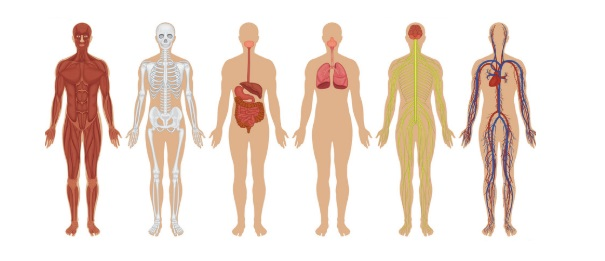
\includegraphics[width = .7\textwidth]{source/images/image22.png}
 	\captionof{figure}{\label{fig:im23}Los sistemas del cuerpo humano.\cite{web11}}
	\end{center} 
\end{figure}

\section{Sistema Digestivo}
La cavidad abdominal 
es el espacio corporal que ocupa la región del abdomen, ubicada entre el diafragma y la abertura de la pelvis. 
Es la cavidad más grande del cuerpo humano 
a diferencia de las demás cavidades,ver \ref{fig:im24}, y 
contiene los principales órganos del aparato digestivo, urinario y genital.
Para su estudio y evaluación clínica en el campo de la medicina, 
el abdomen debe ser dividido topográficamente de forma externa en 9 
cuadrantes o regiones, utilizando cuatro líneas 
trazadas imaginariamente, dos verticales y dos horizontales, ver \ref{fig:im24}.\cite{web12}
\begin{figure}
 \begin{center}
  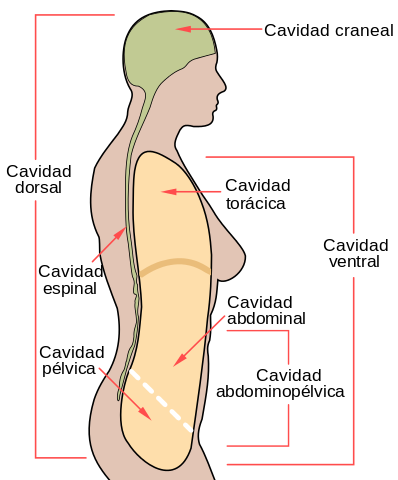
\includegraphics[width = .3\textwidth]{source/images/image56.png}
  \captionof{figure}{\label{fig:im24}Cavidades del cuerpo humano.}
 \end{center} 
\end{figure}

\begin{figure}[H]
	\begin{center}
 		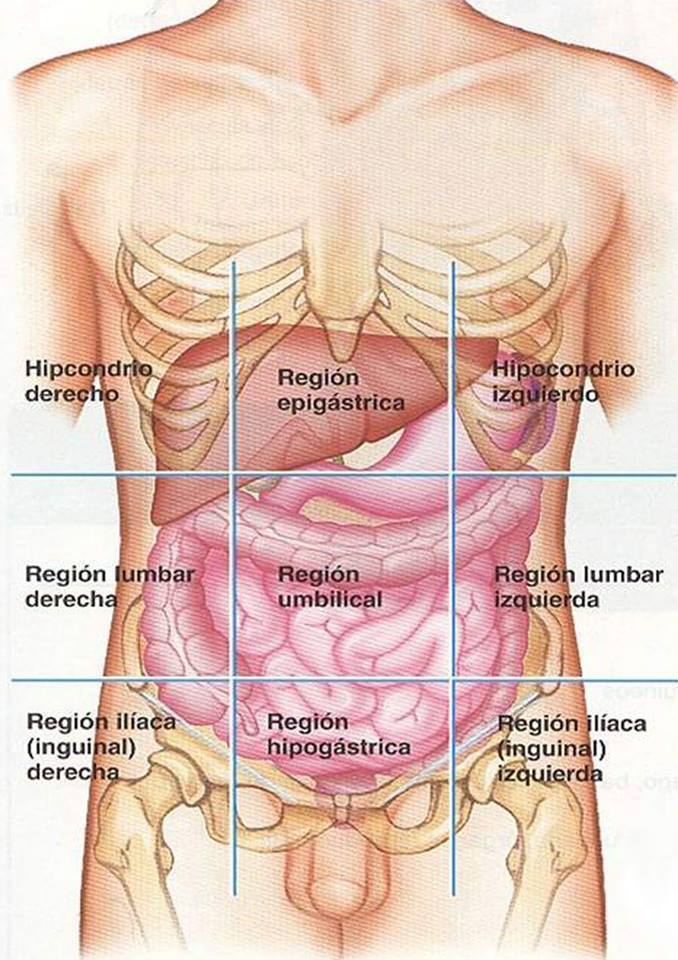
\includegraphics[width = .3\textwidth]{v3/images/image1.jpg}
 		\captionof{figure}{\label{fig:im24.0}Cuadrantes de la cavidad abdominal.}
	\end{center} 
\end{figure}

A continuación se presenta un resumen de los conceptos básicos de los elementos 
que conforman la cavidad abdominal %% TODO: Arreglar esta referencia \cite{}:
\begin{itemize}
	\item El \textbf{abdomen} es la región que se encuentra entre el tórax y la pelvis. El diafragma separa las estructuras del tórax de las del abdomen. 
	\item La \textbf{abertura} superior de la pelvis comunica la pelvis con la cavidad abdominal.
	\item La \textbf{pared abdominal} se encuentra compuesta por piel, tejido subcutáneo, planos musculares con sus aponeurosis y fascias y peritoneo parietal.
	\item La \textbf{cavidad abdominal} se encuentra integrada por la cavidad peritoneal, el retroperitoneo y las vísceras peritonizadas.
	\item La \textbf{cavidad peritoneal} se encuentra limitada por las láminas visceral y parietal del peritoneo.
	\item El \textbf{retroperitoneo} está integrado por todas las estructuras anatómicas que se encuentran por detrás de la lámina parietal posterior del peritoneo.
	\item La \textbf{cavidad abdominal} incluye estructuras pertenecientes a los sistemas digestivo, endocrino, vascular, nervioso y urinario.
	\item Las \textbf{vísceras sólidas} de la cavidad abdominal son el hígado, el bazo, el páncreas, los riñones y las glándulas suprarrenales.
	\item Las \textbf{huecas} son el tubo digestivo y las vías de excreción urinaria. 
	\item El \textbf{tubo digestivo abdominal} está integrado por el esófago (porción abdominal), el estómago, el duodeno, el yeyuno, el íleon y las porciones del colon (ciego, apéndice vermiforme, colon ascendente, transverso, descendente y sigmoide).
	\item El \textbf{sistema vascular} incluye las arterias ramas de la porción abdominal de la aorta, las venas tributarias de la cava inferior y la vena porta hepática y los linfáticos.
	\item La \textbf{porción abdominal de la arteria aorta} se extiende desde el hiato aórtico del diafragma y sus ramas terminales son las arterias ilíacas comunes. Se encuentra en situación prevertebral desplazada hacia la izquierda de la columna lumbar. 
	\item La \textbf{vena cava inferior} se forma por la anastomosis de ambas ilíacas comunes y asciende en situación prevertebral desplazada a la derecha hasta el orificio de la vena cava en el diafragma.
	\item La \textbf{vena porta hepática} se forma detrás de la cabeza del páncreas por la anastomosis de las venas esplénica (que ya recibe como afluente a la vena mesentérica inferior) y mesentérica superior, y se dirige al hígado dentro del omento menor.
	\item Los \textbf{troncos linfáticos} de los miembros inferiores, la pelvis y el abdomen confluyen detrás de la cabeza del páncreas donde se origina el conducto torácico. Este asciende y atraviesa el diafragma por el hiato aórtico en dirección al tórax.
\end{itemize}
A continuación se muestra una imagen,ver \ref{fig:im25}, del sistema digestivo (El epiplón mayor
\footnote{ también llamado omento o reaño, es un pliegue bilaminar del peritoneo situado en el abdomen. Se extiende desde el estómago y la porción proximal de duodeno hasta órganos adyacentes de la cavidad abdominal.} 
ha sido parcialmente eliminado o reflejado)  está contienen la información de cuáles son los órganos y elementos que lo conforman, estos serán 
varios ya que se han tomado como guía, estos elegidos mediante a una entrevista de estudiantes de medicina como material que se ha utilizado para el estudio del cuerpo 
humano, para la realización de modelos en 3D del presente trabajo. ejemplifica el material que dispone pero no limitado a el alumnado para el estudio del sistema en cuestión.\\
\begin{figure}[H]
	\begin{center}
 		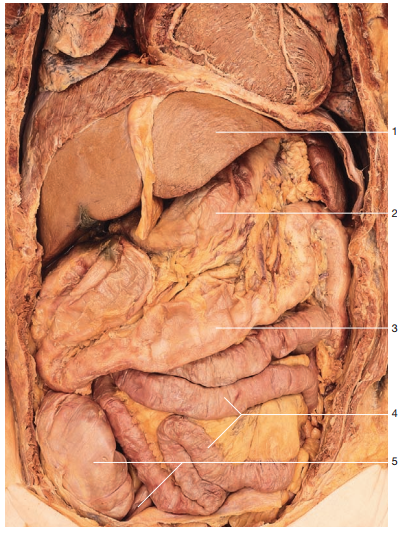
\includegraphics[width = .5\textwidth]{source/images/image72.png}
 		\captionof{figure}{\label{fig:im25}Órganos digestivos in situ\cite{rohen2018anatomy}}
	\end{center} 
\end{figure}
\begin{enumerate}
	\item Hígado
	\item Estómago
	\item Colon transverso
	\item Intestino delgado
	\item Ciego con apéndice vermiforme	
\end{enumerate}
En el apendice se puede encontrar la información detallada de los componentes y organos del sistema digestivo.

\section{Realidad Virtual}
Algunos autores definen así la Realidad Virtual.\\
\newline
\textit{“La realidad virtual (RV) es una simulación tridimensional generada o asistida comúnmente por computadora de algún aspecto del mundo real o ficticio, en el cual 
el usuario tiene la sensación de pertenecer a ese ambiente sintético o interactuar con él”}\cite{web6}\\ 
\textbf{Corrado Padila Érica}\\
\newline
“Realidad Virtual: gráficos 3D en entornos inmersivos que usan I/O
artefactos como guantes, cascos, etc. en busca de mayores grados de iteración
con el ambiente virtual”\cite{web7}\\ 
\textbf{Lozano Miguel, Calderón}\\
\newline
"Realidad Virtual es una forma en que los seres humanos puedan
visualizar, manipular e interactuar con las computadoras y datos extremadamente
complejos".\cite{web8}\\
\textbf{Isdale, Jerry}\\
\newline
“Un sistema interactivo capaz de crear una simulación que implique a varios de los sentidos del ser humano, generados por una computadora, explorable, visualizable y manipulable 
en tiempo real; este bajo la forma de imágenes y sonidos, estos, dando la sensación de presencia en el entorno generado”\cite{web9}\\
\textbf{Levis, Diego}\\
\newline
Esta última ha sido la definición que se ha tomado para el desarrollo del proyecto del trabajo terminal, asimismo se puede concluir que todos los autores coinciden en que la 
realidad virtual es un mundo simulado en el que el usuario puede interactuar en tiempo real por medio
de dispositivos o computadoras que logran un efecto artificial e inmersivo en el que se pueden manipular objetos.

\section{La Realidad Virtual en la Educaci\'on}
Los estudiantes deben aprender que se pueden conquistar nuevas fronteras cruzando los límites disciplinarios. En el caso de la tecnología y el proceso educativo, 
se deben crear oportunidades de aprendizaje que atraviesen la psicología, la sociología, la historia, la filosofía, la antropología, la ciencia y la teoría organizacional, 
construyéndose hacia sistemas complejos de comprensión aplicables a problemas complejos. Esto es tan cierto para comprender a los alumnos individuales como para comprender 
la cultura colectiva.\\
A pesar del potencial de la interacion de tecnologias de la información, en este caso la RV, pueden derivarse de un enfoque integrado y transdisciplinario, 
todavía es necesario ubicar el pro dentro de las estructuras administrativas y los contenidos academicos de la Universidad.\\ 
La inclusión de este topo de tecnologías refleja una imagen de indagación que trasciende y se centra en cuatro amplios dominios de indagación.\cite{norton1994integrating}
\begin{enumerate}
	\item \textbf{Impactos de la tecnología en los contextos sociales}a través de exploraciones de la historia de la tecnología, el papel de la tecnología en el cambio, los impactos sociales, globales, económicos, políticos y psicológicos de la tecnología, la integración de la tecnología a medida que impacta en diversas culturas y las implicaciones de los cambios actuales para el diseño de práctica educativa.
	\item \textbf{Impactos de la tecnología en las formas de conocimiento} a través del examen de las influencias psicológicas y epistemológicas de la tecnología sobre la naturaleza del conocimiento - sobre lo que sabemos y cómo lo conocemos - al indagar sobre la estructura y las implicaciones de las diversas arenas de discurso social y estructural creadas por las tecnologías electrónicas.
	\item \textbf{Impactos de la tecnología en el proceso de aprendizaje} a través de investigaciones de definiciones emergentes de entornos de aprendizaje consistentes con configuraciones sociales más amplias y con visiones más nuevas del proceso de aprendizaje, pensamiento, resolución de problemas y creativo, incluida la naturaleza y el papel de las estrategias de instrucción y concepciones más amplias de los atributos y características del alumno.
	\item \textbf{La tecnología impacta en los objetivos educativos a través de la reevaluación de los objetivos educativos tradicionales}, repensando lo que se debe aprender, cómo se debe aprender, quién es el alumno, la naturaleza de las experiencias culturales de cada alumno y cómo se puede evaluar el aprendizaje, en particular el la naturaleza transdisciplinaria del conocimiento y el aprendizaje y la literatura emergente sobre estándares y metas para la educación, así como el papel de la tecnología en la configuración de estas reevaluaciones.
\end{enumerate}
Todo esto \dots %Pendiente...
\subsection{Participación Programable}
Las características de la realidad virtual son las mismas que las de una buena enseñanza. El profesor quiere crear un entorno que sea programable y en el que 
participen los alumnos. "El principio más importante del diseño de actividades en el aula es que las acciones del estudiante determinan lo que se aprenderá". 
Es decir, la atención es lo primero, el aprendizaje después de la atención está enfocada. Y el aprendizaje es principalmente acción.\\ 
La idea es simple, todo lo que hacemos para educar con palabras y con imágenes se puede brindar como experiencia virtual. Podemos variar ubicación, escala, densidad de información, 
interactividad y capacidad de respuesta, tiempo, grado de participación.\\
La idea es simple, todo lo que hacemos para educar con palabras y con imágenes se puede brindar como experiencia virtual. Podemos variar ubicación, escala, densidad de información, 
interactividad y capacidad de respuesta, tiempo, grado de participación.
\subsection{Semántica Natural}
La interacción de la RV está acoplada al comportamiento natural. La regla general es que un niño debe poder controlar el sistema. Sin líneas de comando o clics del mouse, 
más bien, simplemente caminar y señalar y hablar y agarrar.\\
La realidad virtual tiene sentido cuando lo que un participante ve y oye tiene un significado que no requiere explicación. Piense en una casa. 
Una descripción textual requiere habilidades de lectura, una base de datos de procedimientos (listas de coordenadas) requiere decodificación, una imagen puede reconocerse 
inmediatamente pero no es interactiva. Una casa en realidad virtual se parece más a una casa física, puedes mirarla mientras caminas alrededor, puedes caminar por la puerta 
principal y explorar cada habitación. Una casa física tiene semántica natural, nadie necesita explicarla. La semántica natural es lo que aprende un niño antes de la escolarización 
simbólica.
\subsection{Constructivismo}
Los entornos virtuales no se limitan solo a la visualización, el alumno puede interactuar con objetos y espacios en la realidad virtual. El alumno puede utilizar herramientas para crear 
nuevos entornos, modificar los antiguos, realizar exámenes de simulación, corregir errores, jugar, en lugar de enseñar una estructura de símbolos y luego enseñar el significado de esa 
estructura, en RV. Primero enseñaremos el significado a través de la experiencia, luego (si es necesario) enseñaremos la abstracción simbólica de nuestras experiencias.\\
Pero la computadora es una herramienta ideal para manipular las abstracciones simbólicas. En lugar de enseñar la abstracción, podemos simplemente enseñar cómo usar la herramienta 
de realidad virtual, una interfaz natural con abstracciones. La RV no es una simulación de la realidad, es un superconjunto de la realidad.\\
La realidad virtual enseña la construcción activa del medio ambiente. Los datos no son una lista abstracta de números, los datos son lo que percibimos en nuestro entorno. 
El aprendizaje no es una lista abstracta de palabras de libros de texto, es lo que hacemos en nuestro entorno. El plan de estudios oculto de la realidad virtual es: haz tu mundo y 
cuídalo. Prueba los experimentos de forma segura. Experimente las consecuencias, luego elija del conocimiento lo que sea necesario.
\subsection{Presencia Cognitiva}
En la realidad virtual, cada objeto se puede habitar como un cuerpo virtual. Los estudiantes no son simplemente coparticipantes, trayendo su perspectiva dentro del mismo contexto de un objeto, 
sino que los estudiantes pueden convertirse en el objeto, ver y actuar en el mundo virtual como si fuera el objeto. \cite{bricken1990learning}

\section{Modelado 3D}
En general, independientemente de la disciplina, el proceso de modelado es una simplificación de un objeto para su posterior estudio o representación. 
Así, podemos hablar de modelos matemáticos que simplifican fenómenos físicos, o modelos meteorológicos para la predicción del tiempo atmosférico, etc.
 Un modelo geométrico define la información sobre la forma (geometría) de un determinado objeto. Las simplificaciones que se realicen en su definición 
 vendrán determinadas por diferentes factores como el método de representación utilizado, operadores empleados o nivel de detalle.\cite{web13} \\
Se puede definir el proceso de modelado geométrico tridimensional como el encargado de crear modelos consistentes que puedan ser manejados algorítmicamente 
en un computador. Este proceso de construcción se aborda en diferentes etapas, partiendo típicamente de entidades básicas y aplicando una serie de operadores 
sobre ellas. Estas entidades básicas pueden ser primitivas geométricas (calculadas de forma algorítmica o mediante una ecuación matemática) u obtenidas mediante 
un dispositivo de captura (escáner 3D).\\
Existen multitud de técnicas de modelado 3D. En una primera taxonomía de alto nivel podemos hacer una categorización dependiendo de si el modelado se centra 
en definir únicamente las características del contorno del objeto, los siguiente son los mas usados:\\
\begin{itemize}
\item \textbf{Modelado Sólido:} también conocidos como de Geometría Sólida Constructiva (CSG Constructed Solid Geometry). Los modelos sólidos definen el volumen 
del objeto que representan, y en muchos casos indican incluso el centro de masas, la densidad del material interna, etc. Se utilizan en fabricación por computadora 
y en aplicaciones médicas e industriales.
\item \textbf{Modelado de Contorno:} también conocidos como de Representación de Contorno (B-Rep - Boundary Representation). Los modelos de contorno únicamente 
representan la superficie límite del objeto (de forma conceptual, la "cáscara"). Son más fáciles de definir y modificar. Además, lo interesante para la representación 
del objeto es su apariencia exterior (en los casos donde interesa el interior simplemente se aproxima, como en el caso del SubSurfaceScattering). Prácticamente todos 
los paquetes de diseño y animación (incluido Blender) empleados en síntesis de imagen y en aplicaciones interactivas emplean este tipo de modelos.
\end{itemize}
Para  cubrir las necesidades de los modelos 3D de los órganos del sistema digestivo se ha opto por que estos fueran realizados en el modelado de contorno por su facilidad 
de desarrollo y ligereza de carga en el renderizado en el momento de la implementación de estos en el sistema de realidad virtual.\\

\section{Generacion de Entorno 3D}
El entorno 3D es en donde el usuario se encontrará al ingresar al sistema de realidad virtual, para, este se ha realizado para dar la sensación de encontrarse en un ambiente médico.\\
Se utilizaron modelos ya realizados por un autor adquiriendo los derechos de uso ya que la realización de estos no se consideran parte integral del desarrollo del Trabajo Terminal, 
escrito esto no se quiere demeritar la necesidad de hacer el usuario ya que, como se ha mencionado en secciones anteriores, se tiene énfasis en la experiencia del usuario para que 
la inmersión del usuario sea la mayor posible.\\
\begin{figure}[H]
	\begin{center}
 		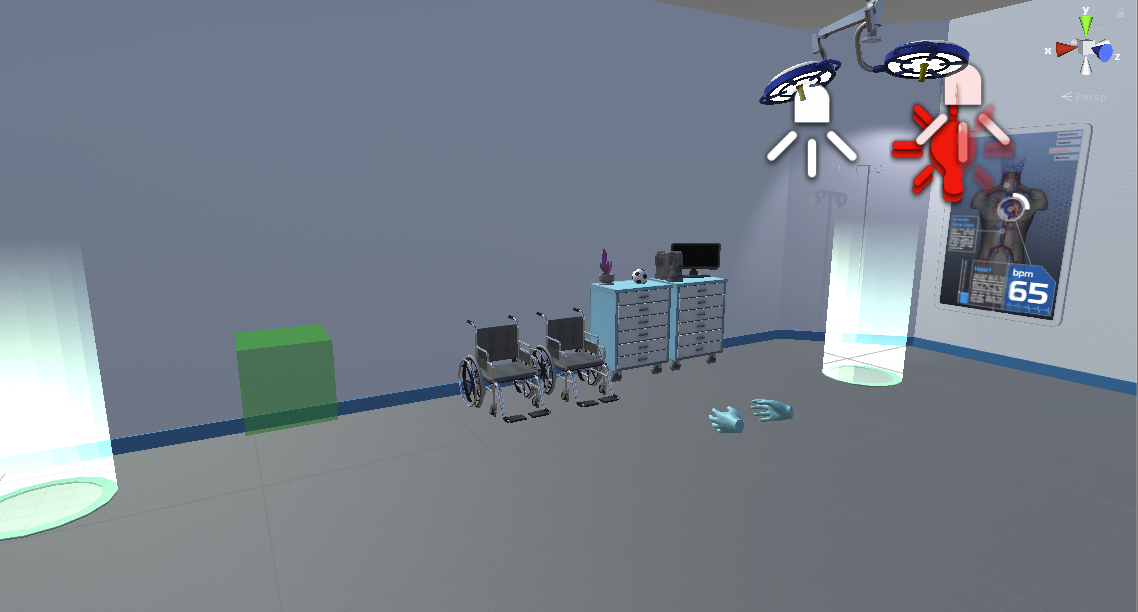
\includegraphics[width = .5\textwidth]{source/images/image63.png}
 		\captionof{figure}{\label{fig:im31}Entorno 3D vista normal}
	\end{center} 
\end{figure}

\begin{figure}[H]
	\begin{center}
 		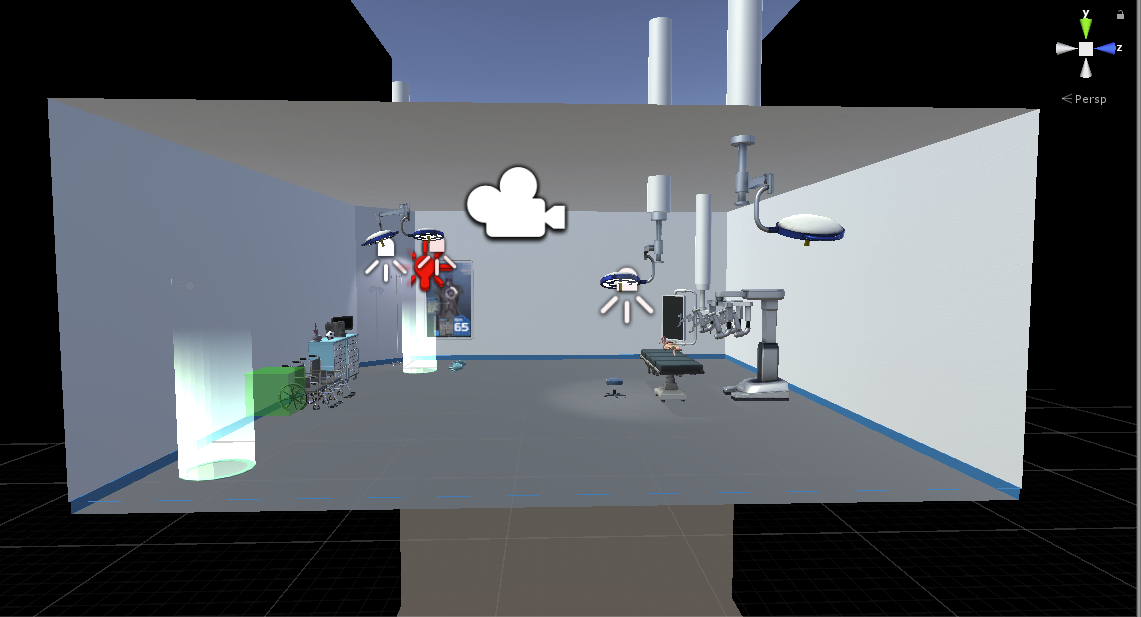
\includegraphics[width = .5\textwidth]{source/images/image53.png}
 		\captionof{figure}{\label{fig:im32} Entorno 3D vista externa de la escena}
	\end{center} 
\end{figure}

\begin{figure}[H]
	\begin{center}
 		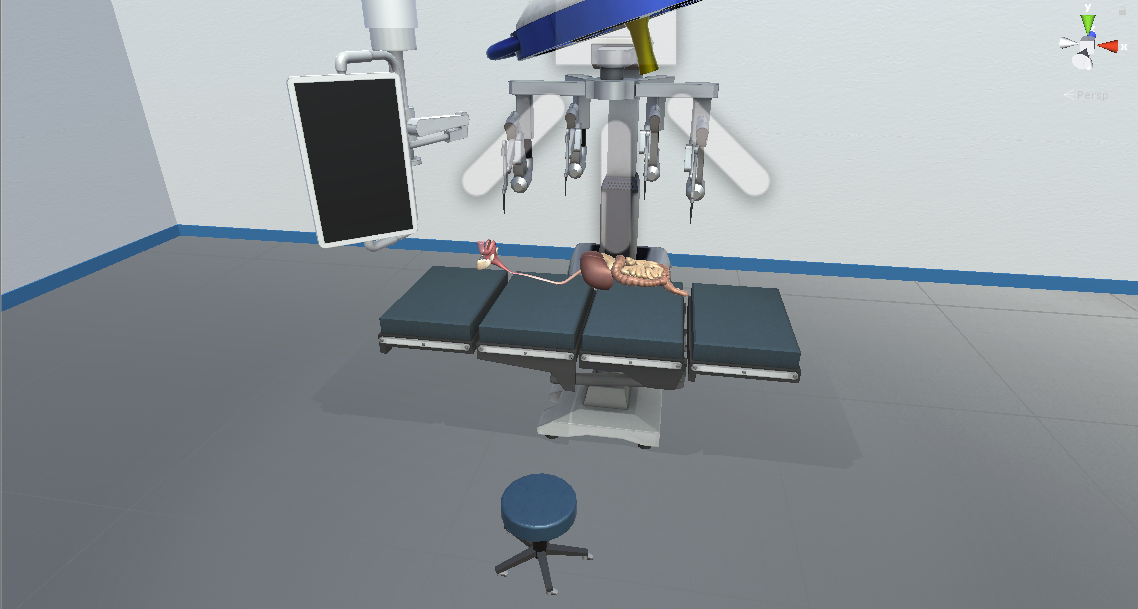
\includegraphics[width = .5\textwidth]{source/images/image16.png}
 		\captionof{figure}{\label{fig:im33}Entorno 3D  vista principal}
	\end{center} 
\end{figure}


% (Aquí puede decir lo de unity y demás cosas que se requieren para hacer lo que usted ya hizo)
%(Tratemos de usar lo que se tiene y solo añadir si es indispensable, recortar si es necesario para añadir a Apendices, como lo de las imagenes del aparato digestivo que estaban en el primer documento)

\chapter{Solución Propuesta}

\section{Propuesta de Solución}
Se elaboró un sistema de realidad virtual del sistema digestivo del cuerpo humano que permite interactuar con modelos tridimensionales.
 La intención es sentar las bases para un sistema de apoyo al aprendizaje que sea más práctico \cite{moore1995learning}, 
 sin sustituir a ningún método de estudio tradicional.\\

\section{Arquitectura del sistema}

\subsection{Diagrama de Despliegue}
Este diagrama representa los dos tipos de elementos, nodos y conexiones, así como la distribución de componentes del sistema 
de información con respecto a la partición física del sistema.\\
\begin{figure}[H]
	\begin{center}
 		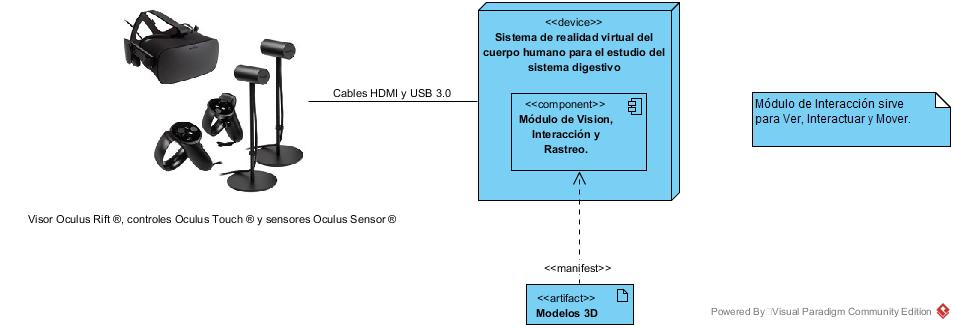
\includegraphics[width = .5\textwidth]{v3/images/cu2.jpg}
 		\captionof{figure}{\label{fig:as1}Diagrama de despliegue del sistema}
	\end{center} 
\end{figure}
Los componentes de este como se pueden apreciiar en la figura \ref{fig:as1} son las siguientes:
\begin{itemize}
  \item \textbf{Dispositivo:}
  \item \textbf{Componentes:}
  \begin{itemize}
    \item Visión
    \item Interacción
    \item Rastreo  
  \end{itemize}
  \item \textbf{Artefacto:}
\end{itemize}

\section{Viabilidad} \label{viab}
También se analizó la factibilidad del proyecto en general. Desde el punto de vista técnico se realizó una evaluación de la tecnología 
actual existente y la posibilidad de utilizarla en el desarrollo del sistema. Además de DirectX versión 11 el cuadro \ref{tab:t23} 
muestra los recursos técnicos necesarios para la ejecución correcta del software:\\
\begin{table}[H]
\centering
\begin{tabular}{|c|c|l|}
\hline
\rowcolor[HTML]{9B9B9B} 
\textbf{Cantidad} &
  \textbf{Recursos} &
  \multicolumn{1}{c|}{\cellcolor[HTML]{9B9B9B}\textbf{Características}} \\ \hline
\cellcolor[HTML]{C0C0C0}1 &
  Computadora Personal de Escritorio &
  \begin{tabular}[c]{@{}l@{}}Tarjeta gráfica discreta, RX480\\ Memoria RAM 16 Gb\\ 5 Puertos USB\\ Procesador de 4 núcleos o mayor\end{tabular} \\ \hline
\cellcolor[HTML]{C0C0C0}1 &
  Sistema de realidad Virtual Oculus Rift &
  \begin{tabular}[c]{@{}l@{}}Visor HMD, controles Touch \\ \\ Sensores Touch.\end{tabular} \\ \
  \label{tab:pc}
\end{tabular}

\caption{ Recursos Técnicos.}
\label{tab:t23}
\end{table}
Económicamente, se determinaron los recursos para desarrollar el sistema así como la comparativa con el uso de cuerpos para su examinación y estudio. Después de un análisis e 
investigación de los costos con la dirección del Área de Morfología en la Escuela Superior de Medicina bajo la asesoría del Dr. Macias Rios se determinó que el costo que se 
tiene para el traslado, mantenimiento, uso e inhumación de los cuerpos es de \$40,000.00 c/u, como se ve en el cuadro \ref{tab:t24}.
\begin{table}[H]
\centering
\begin{tabular}{|
>{\columncolor[HTML]{C0C0C0}}c |l|}
\hline
\multicolumn{2}{|c|}{\cellcolor[HTML]{9B9B9B}\textbf{Costo de uso de cuerpos.}} \\ \hline
Traslado, mantenimiento, uso e inhumación           & \$40,000.00 c/u           \\ \hline
Total                                               & \$40,000.00 c/u           \\ \hline
\end{tabular}
\caption{Costo de cálculo de uso de cuerpos.}
\label{tab:t24}
\end{table}

En el caso del desarrollo e implementación del proyecto se consideró la depreciación, como se observa en el cuadro \ref{tab:t25}.
\begin{table}[H]
\centering
\resizebox{\textwidth}{!}{%
\begin{tabular}{clccccc|c|c|}
\hline
\rowcolor[HTML]{9B9B9B} 
\multicolumn{9}{|c|}{\cellcolor[HTML]{9B9B9B}\textbf{Depreciaciones del Proyecto}} \\ \hline
\rowcolor[HTML]{9B9B9B} 
\multicolumn{4}{|c|}{\cellcolor[HTML]{9B9B9B}\textbf{Equipos de Cómputo}} &
  \multicolumn{5}{c|}{\cellcolor[HTML]{9B9B9B}\textbf{Depreciación}} \\ \hline
\rowcolor[HTML]{9B9B9B} 
\multicolumn{1}{|c|}{\cellcolor[HTML]{9B9B9B}\textbf{Cantidad}} &
  \multicolumn{1}{c|}{\cellcolor[HTML]{9B9B9B}\textbf{Equipos}} &
  \multicolumn{1}{c|}{\cellcolor[HTML]{9B9B9B}\textbf{\begin{tabular}[c]{@{}c@{}}Monto original de \\ Inversión\end{tabular}}} &
  \multicolumn{1}{c|}{\cellcolor[HTML]{9B9B9B}\textbf{\begin{tabular}[c]{@{}c@{}}Valor actual\\  del equipo\end{tabular}}} &
  \multicolumn{1}{c|}{\cellcolor[HTML]{9B9B9B}\textbf{\begin{tabular}[c]{@{}c@{}}Valor a \\ \\ depreciar\end{tabular}}} &
  \multicolumn{1}{c|}{\cellcolor[HTML]{9B9B9B}\textbf{\begin{tabular}[c]{@{}c@{}}\%\\ anual\end{tabular}}} &
  \textbf{\begin{tabular}[c]{@{}c@{}}\%\\ mensual\end{tabular}} &
  \textbf{\begin{tabular}[c]{@{}c@{}}Depresiación\\ mensual\end{tabular}} &
  \textbf{\begin{tabular}[c]{@{}c@{}}Depreciación\\ anual\end{tabular}} \\ \hline
\multicolumn{1}{|c|}{\cellcolor[HTML]{C0C0C0}1} &
  \multicolumn{1}{l|}{\begin{tabular}[c]{@{}l@{}}Computadora de\\ escritorio armada\end{tabular}} &
  \multicolumn{1}{c|}{\$25,054.63} &
  \multicolumn{1}{c|}{\$20,000.00} &
  \multicolumn{1}{c|}{\$5,054.63} &
  \multicolumn{1}{c|}{33.33\%} &
  2.78\% &
  \$ 140.52 &
  \$1,545.72 \\ \hline
\multicolumn{1}{|c|}{\cellcolor[HTML]{C0C0C0}1} &
  \multicolumn{1}{l|}{Laptop HP} &
  \multicolumn{1}{c|}{\$9,999.00} &
  \multicolumn{1}{c|}{\$6,999.00} &
  \multicolumn{1}{c|}{\$3,000.00} &
  \multicolumn{1}{c|}{33.33\%} &
  2.78\% &
  \$ 83.40 &
  \$ 917.40 \\ \hline
\multicolumn{7}{l}{} &
  \textbf{Total:} &
  \$ 2,463.12 \\ \cline{8-9} 
\end{tabular}
}
\caption{Depreciaciones del proyecto.}
\label{tab:t25}
\end{table}

Para ofrecer una experiencia aceptable al momento del uso del equipo de Realidad Virtual 
y el software se proponen los elementos del cuadro \ref{tab:componentes}. La computadora 
que se armó tuvo un costo aproximado de \$25,000.00 MXN, ya considerando los demás componentes.

\begin{table}
\centering
\begin{tabular}{|c|c|}\hline
{\bf Componente} & {\bf Modelo}\\\hline
Procesador & AMD Ryzen 5 1600, 3.20GHz\\\hline
Memoria RAM & 16 Gio DDR4\\\hline
Tarjeta de Video & AMD Radeon RX 480 8Gio\\\hline
\end{tabular}
\caption{Componentes principales de la computadora armada que se usó para el proyecto.}
\label{tab:componentes}
\end{table}

\textbf{Pendiente tabla costos}\\
Además, el sistema de Realidad Virtual con sus componentes tiene un costo que se muestra en el cuadro \ref{tab:t27}.
\begin{table}[H]
  \centering
  \begin{tabular}{|c|c|}
  \hline
  \rowcolor[HTML]{9B9B9B} 
  \multicolumn{2}{|c|}{\cellcolor[HTML]{9B9B9B}\textbf{Sistema de Realidad Virtual}} \\ \hline
  \rowcolor[HTML]{9B9B9B} 
  \textbf{Producto}                          & \textbf{Producto}                     \\ \hline
  Visor Oculus Rift                          & Incluido en el paquete                \\ \hline
  Controles Touch Oculus x 2                 & Incluido en el paquete                \\ \hline
  Sensores Oculus x 2                        & Incluido en el paquete                \\ \hline
  Anexos                                     & Incluido en el paquete                \\ \hline
  \textbf{Total:}                            & \$ 8,821.74                           \\ \hline
  \end{tabular}
  \caption{Costos y contenido del sistema de Realidad Virtual.}
  \label{tab:t27}
\end{table}

Se estimaron los sueldos de programador y modelado, como se observa en el cuadro \ref{tab:t28}.\\
\begin{table}[H]
  \centering
  \resizebox{\textwidth}{!}{%
  \begin{tabular}{ccc|c|c|}
  \hline
  \rowcolor[HTML]{9B9B9B} 
  \multicolumn{5}{|c|}{\cellcolor[HTML]{9B9B9B}\textbf{Sueldos}}                                                                                                                                                                                                                                                                    \\ \hline
  \rowcolor[HTML]{9B9B9B} 
  \multicolumn{1}{|c|}{\cellcolor[HTML]{9B9B9B}\textbf{Puesto}} & \multicolumn{1}{c|}{\cellcolor[HTML]{9B9B9B}\textbf{\begin{tabular}[c]{@{}c@{}}Sueldo\\ Mensual\\ individual\end{tabular}}} & \textbf{\begin{tabular}[c]{@{}c@{}}Cantidad \\ \\ de personal\end{tabular}} & \textbf{Sueldos mensuales totales} & \textbf{6 meses} \\ \hline
  \multicolumn{1}{|c|}{Programador}                             & \multicolumn{1}{c|}{\$25,296.00}                                                                                            & 1                                                                           & \$25,296.00                        & \$151,776.00     \\ \hline
  \multicolumn{1}{|c|}{Modelador 3D}                            & \multicolumn{1}{c|}{\$25,296.00}                                                                                            & 1                                                                           & \$25,296.00                        & \$151,776.00     \\ \hline
  \multicolumn{3}{l}{}                                                                                                                                                                                                                                                      & \multicolumn{1}{l|}{Total}         & \$303,522.00     \\ \cline{4-5} 
  \end{tabular}%
  }
  \caption{Cálculo de Sueldos.
  }
  \label{tab:t28}
\end{table}

\begin{table}[H]
  \centering
  \begin{tabular}{c|c|c|}
  \hline
  \rowcolor[HTML]{9B9B9B} 
  \multicolumn{3}{|c|}{\cellcolor[HTML]{9B9B9B}\textbf{Servicios}}                                       \\ \hline
  \rowcolor[HTML]{9B9B9B} 
  \multicolumn{1}{|c|}{\cellcolor[HTML]{9B9B9B}\textbf{Concepto}} & \textbf{Mensual} & \textbf{11 Meses} \\ \hline
  \multicolumn{1}{|c|}{Luz (kw Consumidos por costo Unitario)}    & \$430            & \$4,730           \\ \hline
  \multicolumn{1}{|c|}{Agua (Lt consumidos por costo unitario)}   & \$200            & \$2,200           \\ \hline
  \multicolumn{1}{|c|}{Teléfono e Internet (renta mensual fija)}  & \$ 450           & \$4,850           \\ \hline
  \multicolumn{1}{l|}{}                                           & Total:           & \$11,780          \\ \cline{2-3} 
  \end{tabular}
  
  \caption{Cálculo de Costo por Servicios.}
  \label{tab:t29}
\end{table}

Los servicios estimados se muestran en el cuadro \ref{tab:t29} y en el cuadro \ref{tab:t210} se muestra la suma total y como resultado se obtiene el costo total del proyecto, 
que se estima en: \$326,316.86.\\
\begin{table}[H]
  \centering
  \begin{tabular}{|l|r|}
  \hline
  \rowcolor[HTML]{9B9B9B} 
  \multicolumn{2}{|c|}{\cellcolor[HTML]{9B9B9B}\textbf{Costos del Proyecto}}                                                    \\ \hline
  \rowcolor[HTML]{9B9B9B} 
  \multicolumn{1}{|c|}{\cellcolor[HTML]{9B9B9B}\textbf{Concepto}} & \multicolumn{1}{c|}{\cellcolor[HTML]{9B9B9B}\textbf{Costo}} \\ \hline
  Servicios                                                       & \$ 11,780                                                   \\ \hline
  Sueldos                                                         & \$303,522.00                                                \\ \hline
  Depreciaciones                                                  & \$2,463.12                                                  \\ \hline
  Equipo extra.                                                   & \$ 8,821.74                                                 \\ \hline
  Total                                                           & \$ 326,316.86                                               \\ \hline
  \end{tabular}
  \caption{Costos finales del proyecto}
  \label{tab:t210}
  \end{table}

En resumen, el costo de usar nueve cuerpos sería de \$360,000.00 y el del proyecto de \$326,318.00, con lo cual se puede considerar viable económicamente.\\

\section{Requerimientos}

\subsection{Funcionales}
\begin{itemize}
  \item Rastreo de controles y visore
  \item Creacion de arcode teleportación
  \begin{itemize}
    \item Teleportacion
  \end{itemize}
  \item Interaccion con órgano (Modelo 3D)
  \begin{itemize}
    \item Inspeccionar órgano
  \end{itemize}
  \item Ver información del órgano
\end{itemize}
\subsection{No Funcionales}
\begin{itemize}
  \item Se utilizará el Sistema de Realidad Virtual Oculus Rift 
  \item Se Utilizará un equipo de cómputo con las caracteristicas del apartado \ref{mod3d} 
\end{itemize}

\section{Casos de Uso}
El planteamiento de casos de uso en un sistema no tradicional como este puede generar un dificultades al momento de expresar cuál es la actividad que podrá 
realizar el actor ya que las  pero se pueden denotar en acciones específicas que queremos que el usuario pueda realizar en el sistema.\\
\begin{figure}[H]
	\begin{center}
 		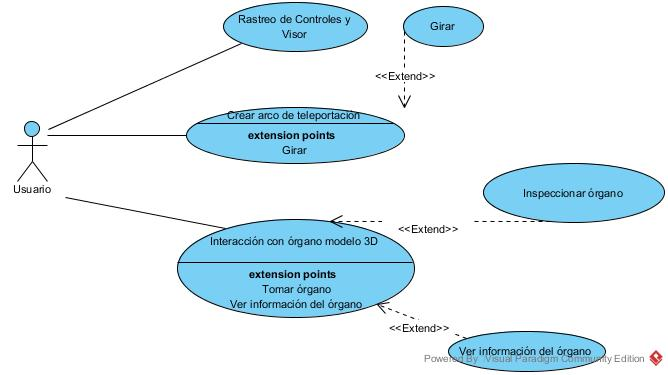
\includegraphics[width = 1\textwidth]{v3/images/cu1.jpg}
 		\captionof{figure}{\label{fig:cu2}Diagrama de casos de uso del sistema}
	\end{center} 
\end{figure}
Ahora bien en la figura \ref{fig:cu2} se muestran los casos de uso que dan parte a el uso del software y las posibilidades generales de interacción en un software de 
Realidad Virtual. Aunque las interacciones dependen eteramente del objetivo del usuario, estas se ven limitadas por las capacidades integradas dentro del software.\\

\section{Metodología}
Recientemente, los productos multimedia digitales, como imágenes, personajes, modelos y animaciones 2D y 3D, se han utilizado ampliamente en muchos dominios, como publicidad, 
películas animadas, edición y diseño de publicaciones, etc. Además, el desarrollo de aplicaciones de software ha utilizado productos multimedia ampliamente. en muchos dominios, 
como marketing electrónico, formación, entretenimiento y juegos, simulación y visualización, y aprendizaje interactivo.\\
En el campo de la informática, la ingeniería de software es una disciplina de ingeniería bien definida que se ocupa de todos los aspectos de la producción de software desde la 
etapa inicial de la especificación de requisitos de software hasta el mantenimiento del software desarrollado después de su implementación \\.
 Por otro lado, el diseño gráfico es un campo de arte que se ocupa de todos los aspectos de la producción multimedia. Prácticamente, la producción multimedia pasa por tres 
 etapas comunes: preproducción, producción y postproducción. Sin embargo, faltan investigaciones que describan estas etapas de forma explícita y estructurada. Además, la 
 descripción de las etapas de producción multimedia no se considera explícitamente en el ciclo de vida del desarrollo de software. De hecho, hay muchas investigaciones de 
 ingeniería de software que abordan productos multimedia, pero se enfocan principalmente en aspectos de modelado y cómo extender el Lenguaje de modelado unificado (UML) 
 para apoyar el modelado de productos multimedia como objetos dentro de aplicaciones de software. \\.
Por lo tanto, existe la necesidad de una metodología de ingeniería interdisciplinaria que tenga como objetivo satisfacer dos pliegues: describir explícitamente las etapas 
de producción de productos multimedia. Integrar las etapas de producción multimedia con el ciclo de vida del desarrollo de software.\cite{al2019multimedia}

\subsection{Metodología de Ingeniería de Software Multimedia}
\subsection{Características de los Productos Multimedia}
Los productos multimedia se pueden clasificar en dos categorías: productos interactivos y no interactivos. Los productos no interactivos también se pueden clasificar 
en productos estáticos  como carteles, logotipos, folletos, modelos estáticos 3D, etc., y productos basados en el tiempo. \cite{engels2002object,sauer2001uml}.\\
Los productos multimedia interactivos son aplicaciones de software que contienen productos multimedia\cite{miranda2017diseno} (es decir, aplicaciones basadas en eventos como juegos, 
aplicaciones web basadas en multimedia y materiales de aprendizaje multimedia basados en interactividad). La figura \ref{fig:me2} a continuación ilustra los tipos de 
productos multimedia.\\
\begin{figure}[H]
	\begin{center}
 		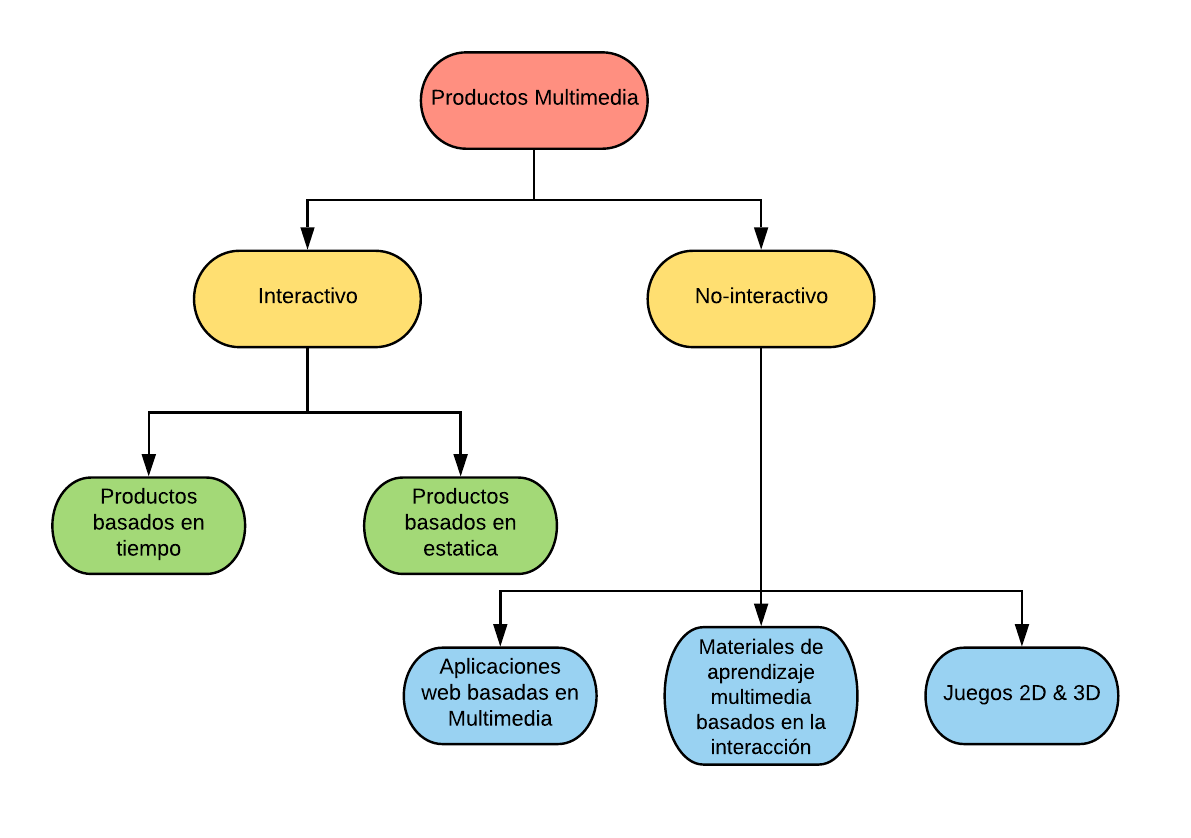
\includegraphics[width = 1\textwidth]{v2/images/image60.png}
 		\captionof{figure}{\label{fig:me2}Tipos de productos multimedia}
	\end{center} 
\end{figure}
Cada una de las categorías anteriores tiene un conjunto de características que pueden  clasificarse en tres dimensiones: vista externa, flujo de acciones y roles de los usuarios.\\
La vista externa se refiere a la forma en que el usuario interactúa con el producto. En este sentido, los usuarios interactúan con productos no interactivos de una manera.\\
Los usuarios suelen realizar eventos y la respuesta del producto a estos eventos mediante acciones.\\
%Un flujo de acciones se refiere al orden en que se muestran los marcos de los productos a los usuarios. En productos estáticos, no hay flujo de acciones, ya que los usuarios leen 
%ven un marco. Sin embargo, los flujos de acciones para productos basados ​​en el tiempo son una secuencia de cuadros. Por otro lado, el flujo de acciones 
%para los productos interactivos podría ser una secuencia, selectiva, iterativa e impulsada por eventos\cite{aleem2016game,cartwright1996pre}.\\
Los roles de los usuarios se refieren a lo que los usuarios pueden hacer para interactuar con productos multimedia. En los productos no interactivos, los usuarios son pasivos donde 
solo pueden leer / mirar productos. Sin embargo, los usuarios son usuarios activos con productos interactivos donde pueden realizar eventos. El cuadro \ref{tab:met1}  resume los tipos de productos 
multimedia y sus características.
\begin{table}[H]
  \resizebox{\textwidth}{!}{%
  \begin{tabular}{|
  >{\columncolor[HTML]{9B9B9B}}c |c|c|c|}
  \hline
  \cellcolor[HTML]{9B9B9B}                                                         & \multicolumn{3}{c|}{\cellcolor[HTML]{9B9B9B}\textbf{Características Multimedia}}                                                                                                                               \\ \cline{2-4} 
  \multirow{-2}{*}{\cellcolor[HTML]{9B9B9B}\textbf{Tipos de productos multimedia}} & \cellcolor[HTML]{9B9B9B}\textbf{Vista Externa} & \cellcolor[HTML]{9B9B9B}\textbf{Flujo de acciones}                                                   & \cellcolor[HTML]{9B9B9B}\textbf{Roles de los Usuarios} \\ \hline
  \textit{Productos estáticos}                                                     & Un cuadro                                      & Sin acciones                                                                                         & Pasivo (ver/leer)                                      \\ \hline
  \textit{Productos basados en tiempo}                                             & Múltiples cuadros                              & Secuencia                                                                                            & Pasivo(mirar)                                          \\ \hline
  \textit{Productos interactivos}                                                  & Impulsado por eventos                          & \begin{tabular}[c]{@{}c@{}}Secuencia, Selectiva, Interactiva e\\  Impulsada por eventos\end{tabular} & Activo(Realiza eventos)                                \\ \hline
  \end{tabular}%
  }
  \caption{Características de los productos multimedia.
  }
  \label{tab:met1}
  \end{table}

  \subsection{Características de la Metodología de ingeniería de software multimedia}
  \subsection{Requisitos y preproducción}
  El objetivo de esta fase es tener muy en claro cuales son los alcances y lo que será posible que el proyecto realice. Para ello se  realizaron las siguientes actividades:\\

\section{Selección de estrategia de diseño}
Al intentar comprender y desarrollar ideas relevantes para los temas, es necesario reiterar la comprensión de sus definiciones actuales y contexto histórico.\\
Con respecto a la realidad virtual, una de las cosas básicas a considerar es la forma en que nuestros sentidos sirven como la entrada que nuestro cerebro utiliza 
para construir una comprensión del mundo que nos rodea. La vista, el oído, el tacto, el olfato y el gusto son el conjunto de estímulo externo más ampliamente aceptado 
que percibe el cuerpo humano.\\
Estos sentidos y nuestras reacciones a ellos son el resultado de milenios de selección natural y hay varias consecuencias de esto incorporadas en nuestro instinto. 
Todo esto es un conocimiento relativamente común y parece que no es necesario reiterar aquí, pero lo importante es afirmar que nosotros, como humanos, tenemos ciertos 
resultados predecibles basados en ciertos conjuntos de entradas. Esencialmente, es instinto, naturaleza humana.\\
Un sitio web bien diseñado utilizará de manera similar el color, la distancia y la tipografía para comunicar claramente un propósito y, a menudo, persuadir algún tipo de acción.\\
Para que todo esto sea efectivo, se deben implementar y descubrir principios de diseño razonables. Existen varios principios para el diseño que pueden traducirse de otros medios. 
El diseño de impresión, el diseño web, la arquitectura, el diseño de interiores, el teatro, los gráficos en movimiento, etc., tienen elementos que pueden considerarse 
relevantes y adoptados. \cite{web18} \\
Al mismo tiempo, el medio de la realidad virtual como propiedades, como la capacidad de intersección del contenido, son únicas.\\
Es por esto que el diseño de un sistema de realidad virtual presenta retos los cuales son difíciles de sobrellevar ya que se tiene que crear una experiencia para el 
usuario en el sistema mismo lo cual conlleva a la selección de una estrategia de diseño centrada en la UX del usuario.

\section{Requisitos para el Desarrollo de Software para Proveer una Experiencia de Realidad Virtual}
La realización una experiencia de realidad alternativa es la prueba definitiva para diseñar una experiencia de usuario impecable que pueda sumergir los sentidos y 
“engañar” a la mente para que abrace la falsa realidad. \\
Pero crear una experiencia de realidad virtual es mucho más complejo que la producción visual 2D y 3D normal asociada con películas y videojuegos, que nos presenta 
como desarrolladores y diseñadores un conjunto completamente nuevo de desafíos. Crear una experiencia de realidad virtual exitosa requiere que el pensamiento actual 
sobre UX evolucione para acomodar sus capacidades y requisitos ya que es una rama la cual, frecuentemente, no es estudiada a profundidad dentro de la carrera de 
Ingeniería en Sistemas Computacionales. 

\subsection{Los cuatro núcleos del diseño UX para RV}
Se plantean cuatro consideraciones centrales para el diseño de experiencias de realidad virtual:\\

\subsection{Interactivo y Reactivo}
La pantalla estereoscópica de visión amplia de los visores de realidad virtual, en este caso específico el Oculus Rift ®,  crea una imagen tridimensional que fomenta 
la profundidad y la perspectiva. El software RV debe seguir constantemente los movimientos de la cabeza y los ojos del usuario, permitiendo que las imágenes se muevan 
y cambien con cada nueva perspectiva, produciendo retroalimentación visual y creando una ilusión de sensación táctil.\\
La experiencia es altamente interactiva y reactiva porque el diseño responde a los movimientos de un usuario y, por lo tanto, siempre está cambiando.\\
Es por eso que una experiencia de realidad virtual se diseña a una vista de 360 grados. Cuando se está diseñando una experiencia, se debe de anticipar y dirigir cada 
movimiento del usuario, teniendo en cuenta dónde dirigir el ojo usando la vista, el sonido se presenta dentro del sistema que está proveyendo la experiencia de realidad virtual.

\subsection{Comodidad y Facilidad}
La cualidad más importante para crear cualquier diseño UX exitoso, especialmente en realidad virtual, es garantizar que el usuario se sienta cómodo durante toda la experiencia\cite{antonya2007design},
 lo que le permite tener un control completo de todos los movimientos y reducir la posibilidad de cinetosis.\\
Los cambios de brillo y los desajustes de velocidad son muy importantes. De hecho, la posibilidad de cinetosis fue un obstáculo importante para el desarrollo de la tecnología de 
Realidad Virtual.\\
Se debe implementar la capacidad de ver y usar controles, hacer clic en botones y otras características centradas en el diseño para evitar confundir o frustrar a los usuarios.\\
En otras palabras, dar al usuario la capacidad y la facilidad de controlar completamente su propia experiencia. Esa es la capacidad del sistema realidad virtual en el cual se 
intenta proveer la capacidad de experimentar completamente un mundo diferente y controlar cada uno de los movimientos del usuario dentro de ese mundo.

\subsection{Escala de texto e imagen}
La percepción actual de software realizado en realidad virtual es que este es "realista". Esto esencialmente está tratando de crear una experiencia que envuelve completamente al usuario.\\
Los detalles importan en el diseño de los sistemas, especialmente uno que sea lo suficientemente intuitivo para requerir la mínima curva de aprendizaje para el usuario.\\
Todas las imágenes deben ser claras y fácilmente legibles, evitando la fatiga visual y teniendo en cuenta la perspectiva. Agregar más y más detalles a un objeto a medida 
que el usuario se acerca a él ayudará a establecer una profundidad realista (y viceversa). El usuario notará mejor el texto grande, en negrita y colorido.

\subsection{Sonido}
La música y los efectos de sonido de alta calidad son una característica fundamental para fomentar la inmersión en la experiencia.\\
Mediante la implementación de 3D efectos de audio a RV audio posicional, el usuario sabrá la dirección en la que ciertos sonidos son originados en relación a donde están, 
o el audio podría ser hecho a sonar como es proveniente de todo tipo de direcciones, dando al usuario la ilusión de estar en medio de un entorno particular.\\
Dar a los usuarios un control de volumen también puede ser una buena idea para ayudar al usuario a encontrar un rango cómodo, aunque estos no son esenciales dentro del sistema.

\section{Retos de realidad virtual para anticipar}
A medida que los diseñadores y desarrolladores se sumergen más en la realidad virtual, este tipo de experiencia relativamente desconocida seguramente se utilizará de formas que 
aún no se han considerado y, por lo tanto, se tendrán desafíos y beneficios que aún no se han descubierto. Sin embargo, pruebas realizadas por usuarios\cite{wen19} han traído a la 
superficie desafíos de diseño actuales.\\
Si bien el objetivo de una experiencia de realidad virtual efectiva y placentera se logra utilizando los principios fundamentales de UX, crear realidad virtual es más fácil 
decirlo que hacerlo.\\
Al realizar el diseño se procura minimizar diligentemente las frustraciones y la confusión de los usuarios al agrupar los detalles y la funcionalidad del usuario en cada 
centímetro del diseño reactivo.

\subsection{Crear un Entorno que se Vea y se Sienta Real}
No ignorar ningún detalle y siempre dé a los usuarios un control completo. Un sistema de realidad virtual es altamente interactivo de 360 grados debe parecer tan realista que los 
usuarios olviden que es realidad virtual. \\
Ofrecer al usuario la capacidad de interactuar de todas las formas posibles, incluida la capacidad de tocar, levantar y lanzar todo tipo de objetos.

\subsection{Asegurar que los Usuarios no Sufran Cinetosis}
La cinetosis ocurre cuando las señales de movimiento físicas y visuales le dan al usuario información adversa. Las claves para evitar que los usuarios se enfermen por el movimiento 
mientras usan un sistema de realidad virtual son el seguimiento efectivo de la cabeza, que mantiene algunos objetos en posiciones fijas sin importar el movimiento del usuario.\\
Además, mantener una velocidad de fotogramas alta y nunca perder fotogramas. Otras formas de combatir la enfermedad de la simulación es minimizar el movimiento de la periferia 
en el diseño y no intentar acelerar al usuario (también conocido como: no simular cambios en la velocidad).

\subsection{Desarrollar controles y menús fáciles de usar}
Este es un desafío en el que los diseñadores todavía están trabajando y se ha diseñado de la mejor forma posible tomando en cuenta diferentes estrategias y modelos de diseño.\\
Dado que los menús de navegación y otros controles no se pueden colocar en las esquinas de la pantalla, ya que en un sistema de realidad virtual, no hay esquinas o puntos finales 
para su vista, deben permanecer fácilmente accesibles y fáciles de usar.\\
Algunos juegos de realidad virtual colocan los controles en las manos de realidad virtual del usuario y la navegación del menú se realiza con la cabeza.\\
Sea lo más creativo posible con la experimentación, pero si los controles y los menús son difíciles de operar o encontrar, lo más probable es que su diseño de RV reciba un gran 
reconocimiento de los usuarios. Un tutorial rápido antes de la experiencia puede ayudar a bordo del usuario para evitar la frustración.

\subsection{Mantener al usuario seguro}
Si bien los usuarios explorarán nuevos espacios, la realidad física es que el cuerpo del usuario todavía está atrapado dentro de una sala de la habitación donde se instale el sistema 
de realidad virtual.\\
Se tiene que asegurarse de que la experiencia de realidad virtual no representa serias amenazas de seguridad para los usuarios.\\
Hacer que funcione para los usuarios. Es importante tener en cuenta las diferentes alturas y tamaños de las personas. No colocar artículos críticos fuera del alcance de usuarios con 
una altura diferente. Además, se debe de tener en cuenta las diferentes preferencias y desventajas físicas al crear varios modos y permitir que los usuarios se sienten mientras visitan 
una realidad alternativa.

\section{Diseño y Desarrollo de Componentes Multimedia}
El diseño de los modelos de los organos fue realizado basado en el material del cual se realizo la investigación en la sección \ref{mod3d} con el método de
Modelado de Contorno ya que este nos permite reducir la cargga de trabajo del motor de Unity, así como el de la tarjeta gráfica.\\

\subsection{Modelos 3D de los Organos}
Los componentes multimedia desarrollados son modelos 3D los cuales son miembros del sistema digestivo del ser humano, 
el sistema digestivo incluye a los órganos del tubo alimenticio y glándulas de secreción exocrina y endocrina.\\

\subsection{Glándulas Salivales}
 continuación se muestran las figuras del resultado final del desarrollo de las glándulas salivales del sistema digestivo 
 en el software de modelado en 3D llamado “Blender”, este fue realizado basado en el material anteriormente provisto.\\
\begin{figure}[H]
	\begin{center}
 		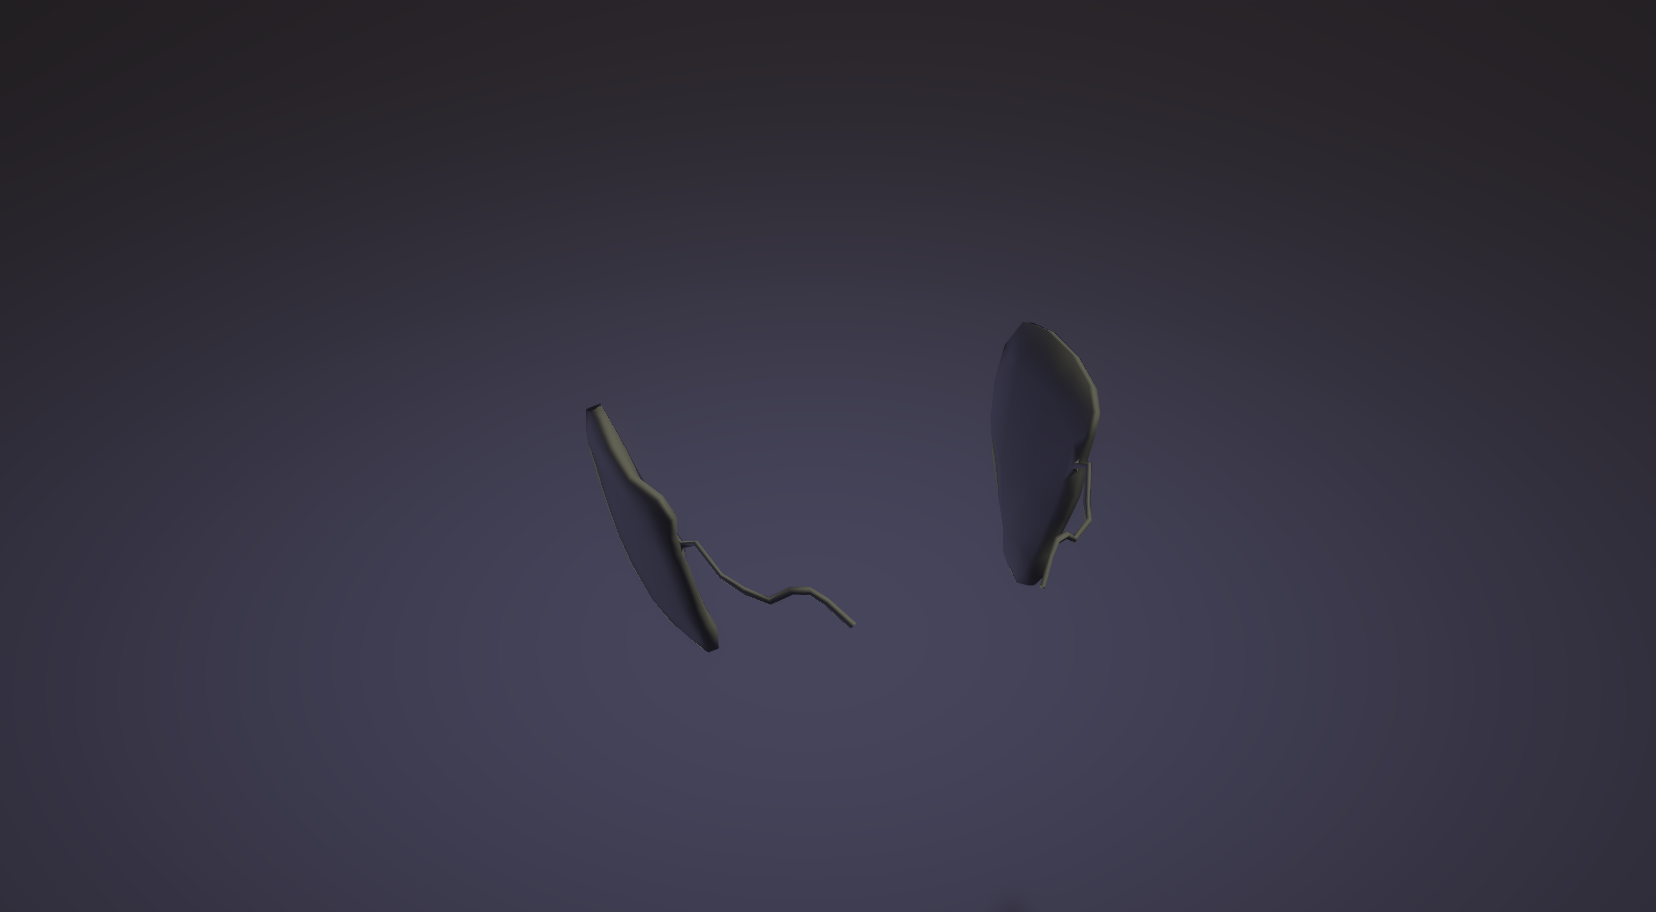
\includegraphics[width = .5\textwidth]{source/images/image41.png}
 		\captionof{figure}{\label{fig:im34}Modelo 3D de las glándulas salivales}
	\end{center} 
\end{figure}

\subsection{Cavidad oral y faringe}
A continuación se muestran las figuras del resultado final del desarrollo de la cavidad oral del sistema digestivo en el software de modelado en 3D llamado “Blender”, este fue realizado basado en el material anteriormente provisto.\\
\begin{figure}[H]
	\begin{center}
 		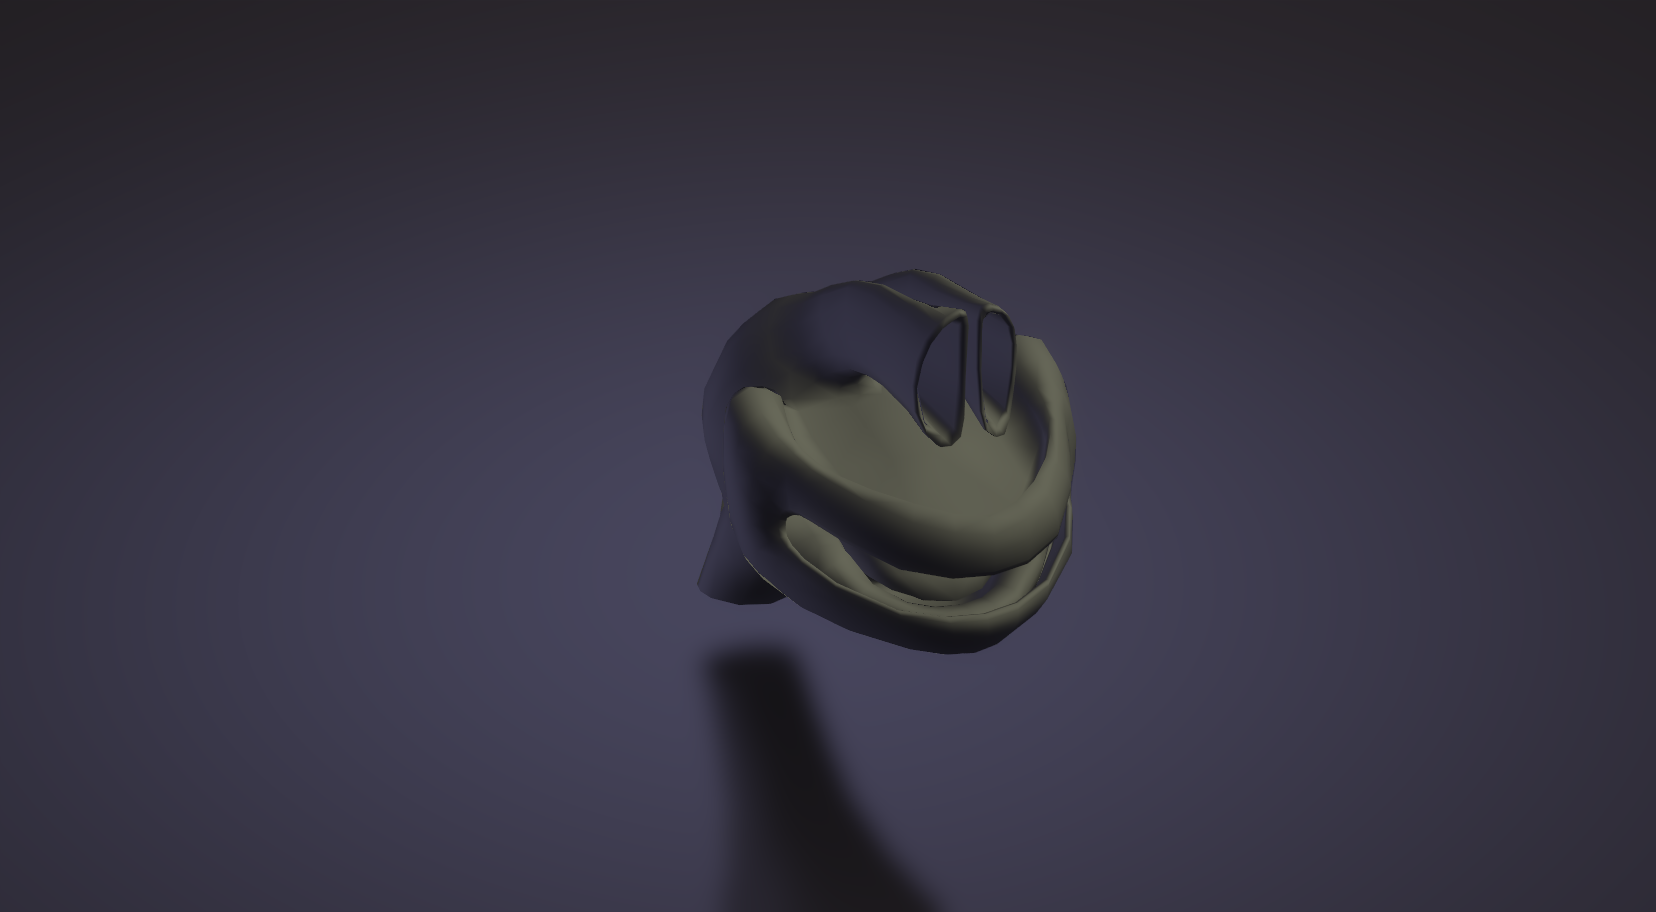
\includegraphics[width = .5\textwidth]{source/images/image14.png}
 		\captionof{figure}{\label{fig:im35}Modelo 3D de la cavidad oral}
	\end{center} 
\end{figure}

\subsection{Esófago}
A continuación se muestran las figuras del resultado final del desarrollo del esófago del sistema digestivo en el software de modelado en 3D llamado “Blender”, este fue realizado basado en el material anteriormente provisto.\\
\begin{figure}[H]
	\begin{center}
 		
\includegraphics[width = .5\textwidth]{source/images/image25.png}
 		\captionof{figure}{\label{fig:im36}Modelo 3D del esófago}
	\end{center} 
\end{figure}

\subsection{Estómago}
A continuación se muestran las figuras del resultado final del desarrollo del estómago del sistema digestivo en el software de modelado en 3D llamado “Blender”, este fue realizado basado en el material anteriormente provisto.\\
\begin{figure}[H]
	\begin{center}
 		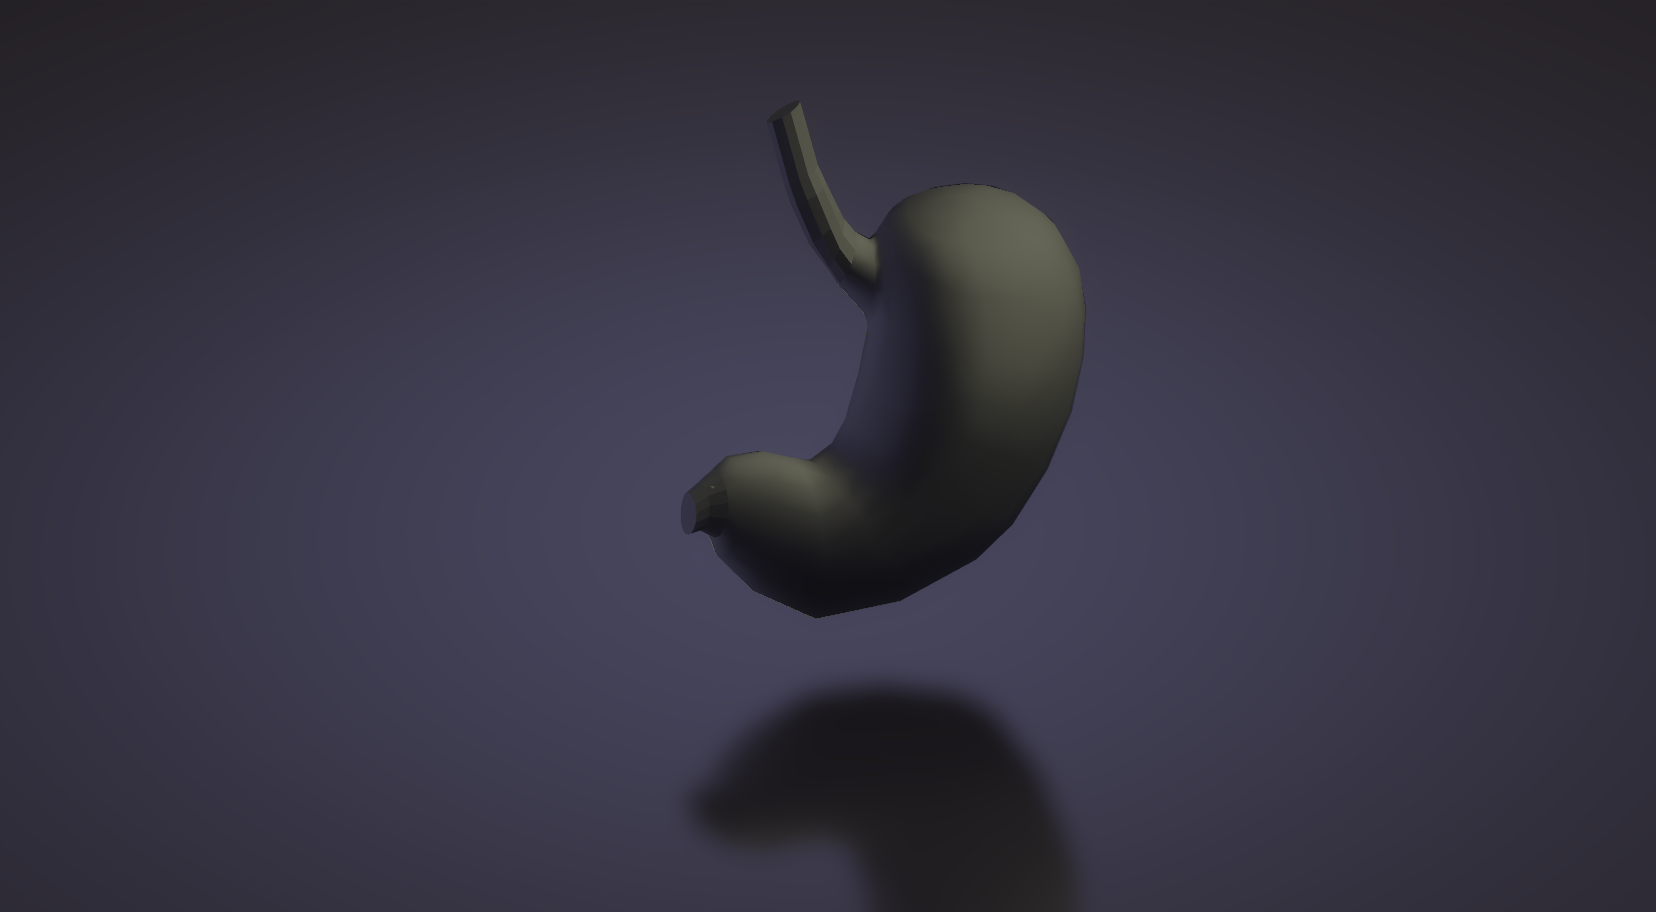
\includegraphics[width = .5\textwidth]{source/images/image42.png}
 		\captionof{figure}{\label{fig:im37} Modelo 3D del estómago }
	\end{center} 
\end{figure}

\subsection{Intestino delgado}
A continuación se muestran las figuras del resultado final del desarrollo del intestino delgado del sistema digestivo en el software de modelado en 3D llamado “Blender”, este fue realizado basado en el material anteriormente provisto.\\
\begin{figure}[H]
	\begin{center}
 		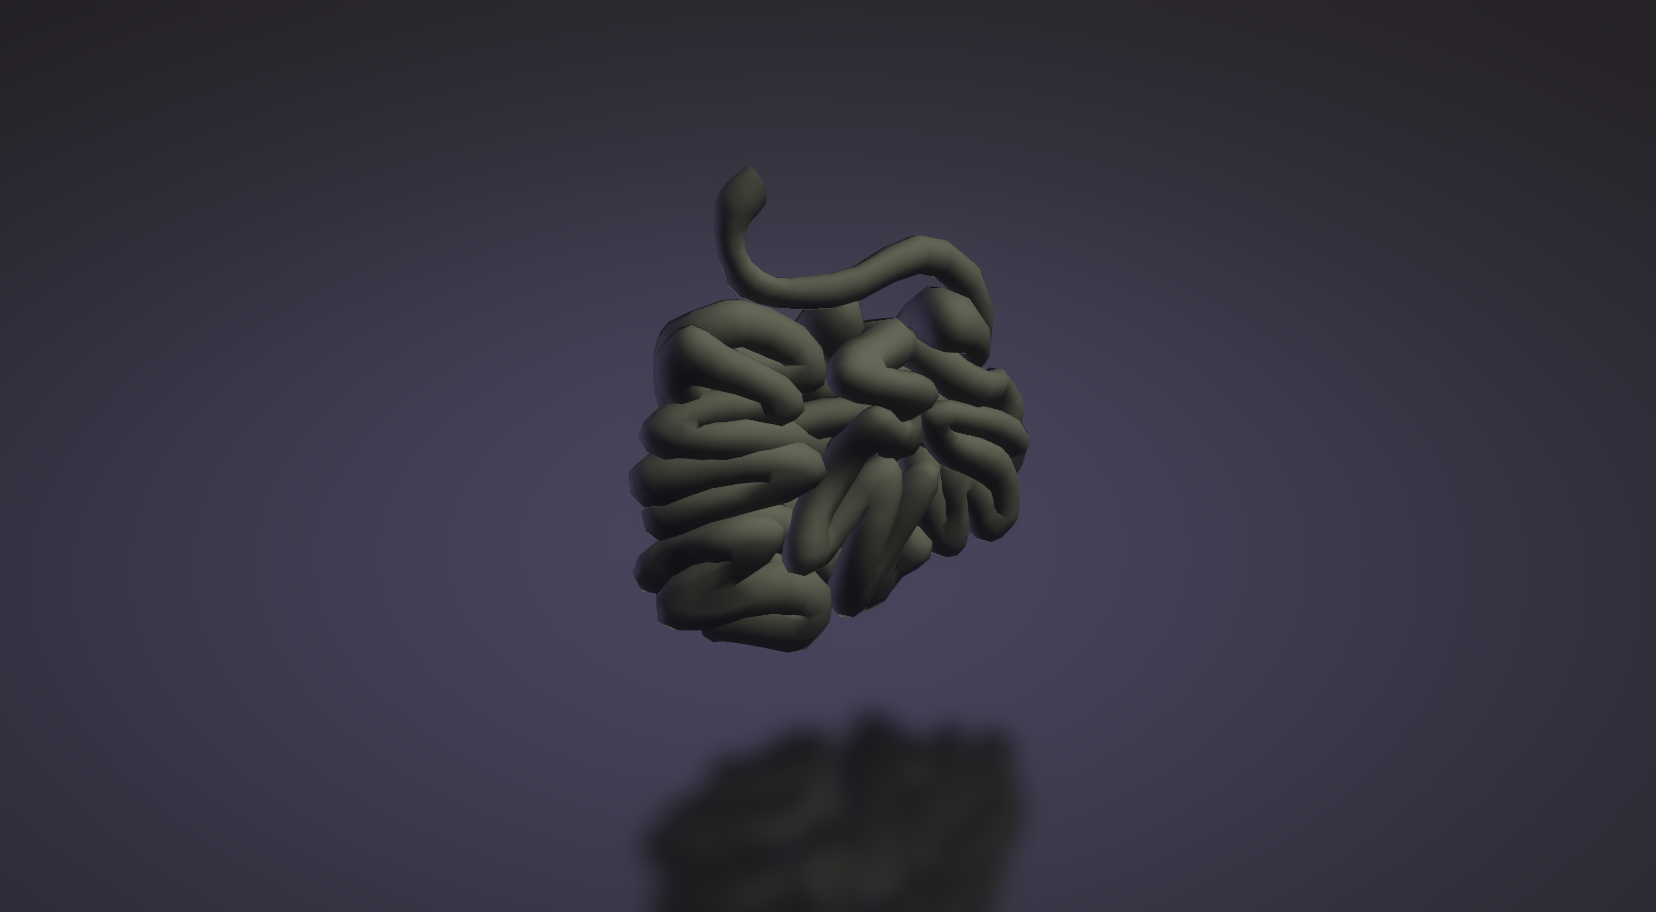
\includegraphics[width = .5\textwidth]{source/images/image69.png}
 		\captionof{figure}{\label{fig:im38}Modelo 3D del intestino delgado}
	\end{center} 
\end{figure}

\subsection{Hígado}
A continuación se muestran las figuras del resultado final del desarrollo del hígado del sistema digestivo en el software de modelado en 3D llamado “Blender”, este fue realizado basado en el material anteriormente provisto.\\
\begin{figure}[H]
	\begin{center}
 		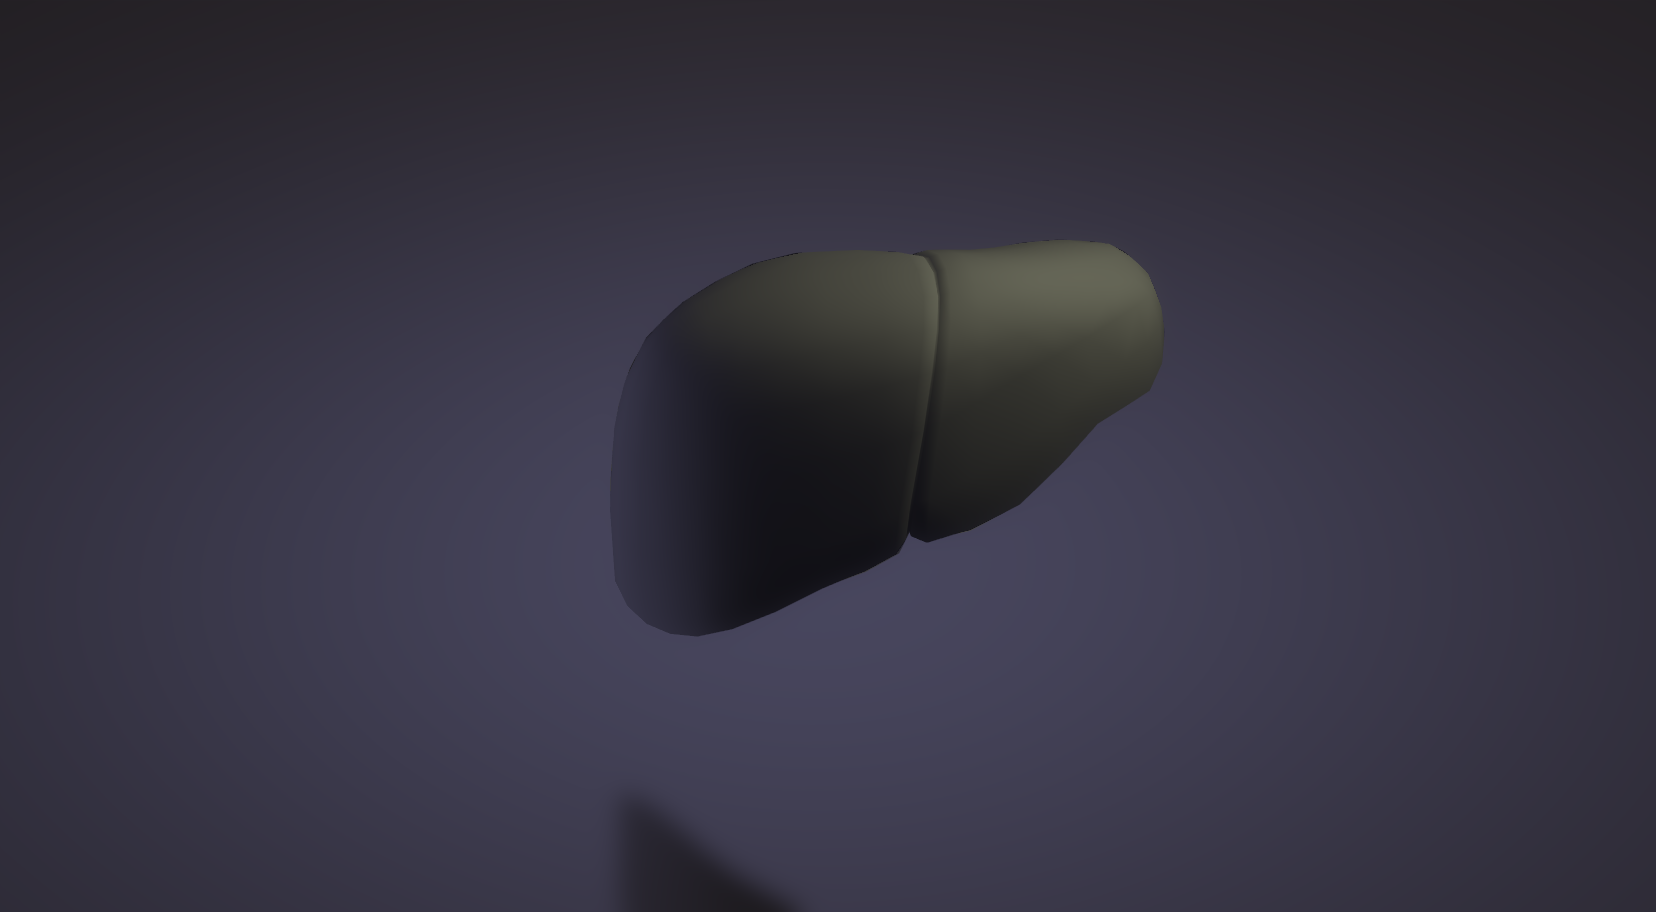
\includegraphics[width = .5\textwidth]{source/images/image17.png}
 		\captionof{figure}{\label{fig:im39}Modelo 3D del hígado}
	\end{center} 
\end{figure}

\subsection{Páncreas}
A continuación se muestran las figuras del resultado final del desarrollo del páncreas del sistema digestivo en el software de modelado en 3D llamado “Blender”, este fue realizado basado en el material anteriormente provisto.\\
\begin{figure}[H]
	\begin{center}
 		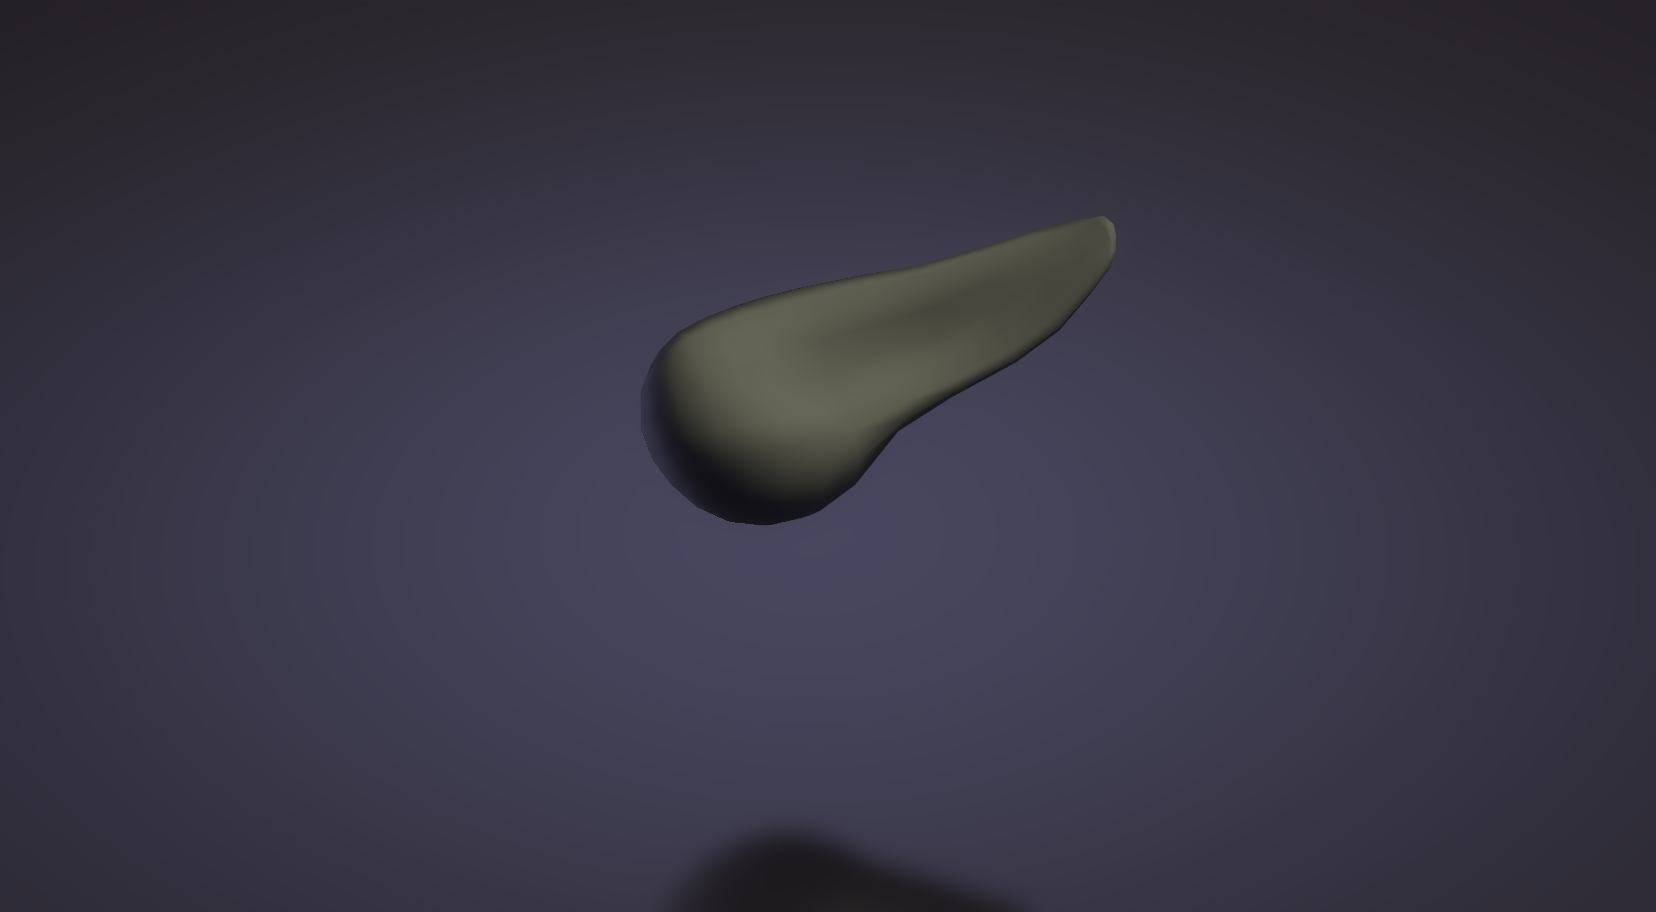
\includegraphics[width = .5\textwidth]{source/images/image19.png}
 		\captionof{figure}{\label{fig:im310}Modelo 3D del páncreas}
	\end{center} 
\end{figure}

\subsection{Vesícula Biliar}
A continuación se muestran las figuras del resultado final del desarrollo de la vesícula biliar del sistema digestivo en el software de modelado en 3D llamado “Blender”, este fue realizado basado en el material anteriormente provisto.\\
\begin{figure}[H]
	\begin{center}
 		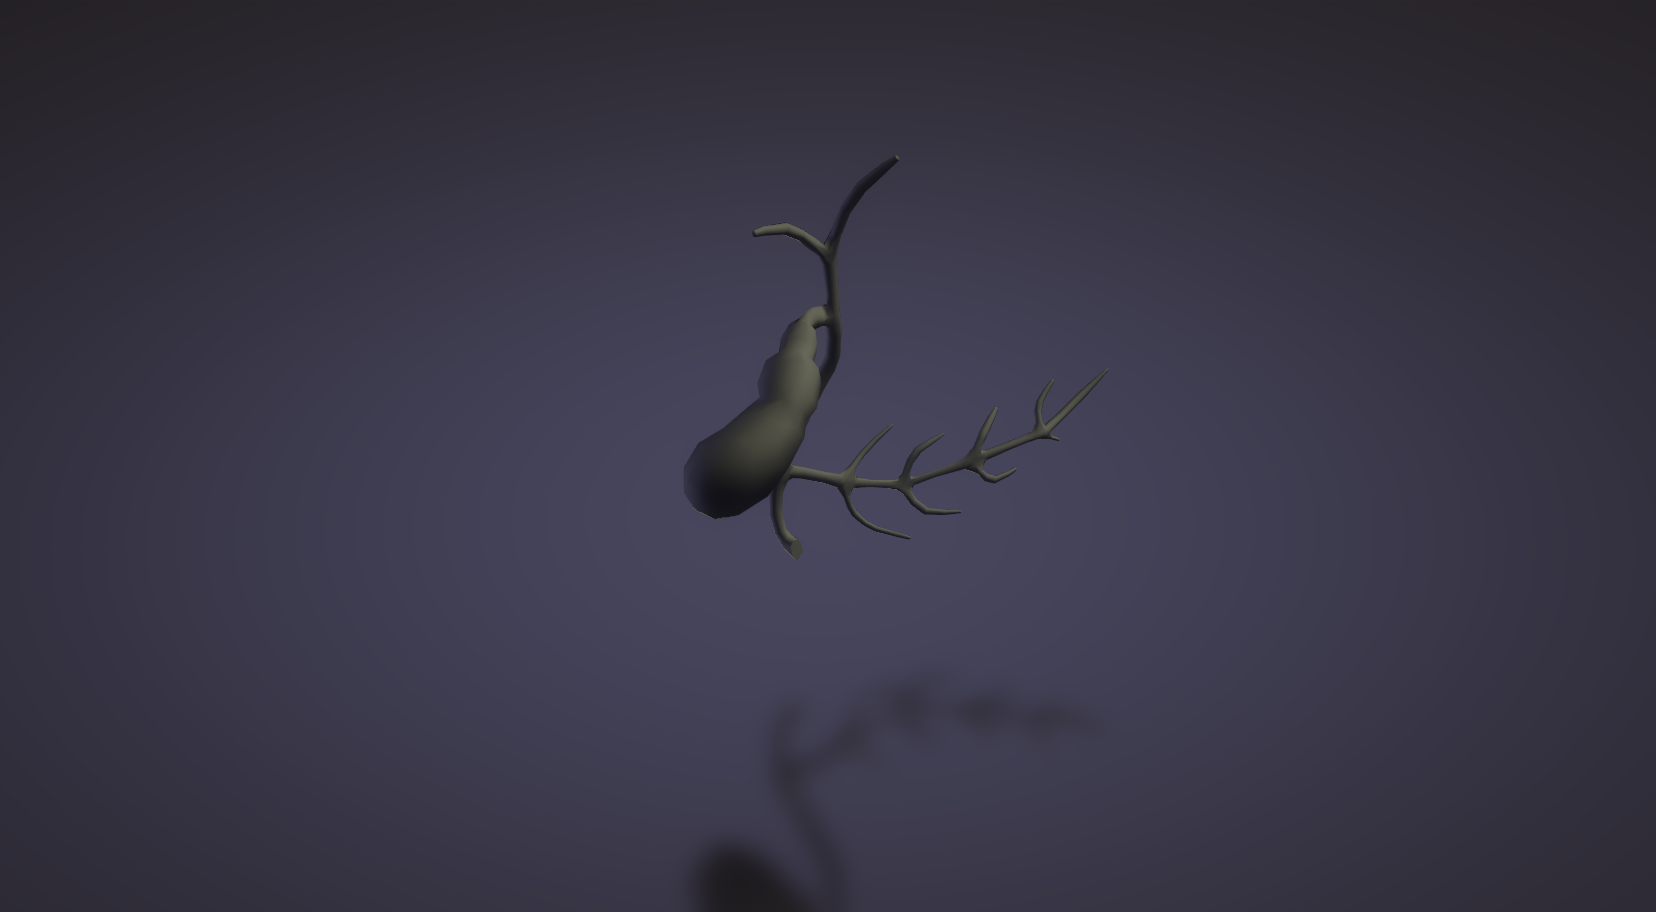
\includegraphics[width = .5\textwidth]{source/images/image26.png}
 		\captionof{figure}{\label{fig:im312}Modelo 3D de la vesícula biliar}
	\end{center} 
\end{figure}

\subsection{Intestino Grueso y Ano}
A continuación se muestran las figuras del resultado final del desarrollo del intestino grueso y ano del sistema digestivo en el software de modelado en 3D llamado “Blender”, este fue realizado basado en el material anteriormente provisto.\\
\begin{figure}[H]
	\begin{center}
 		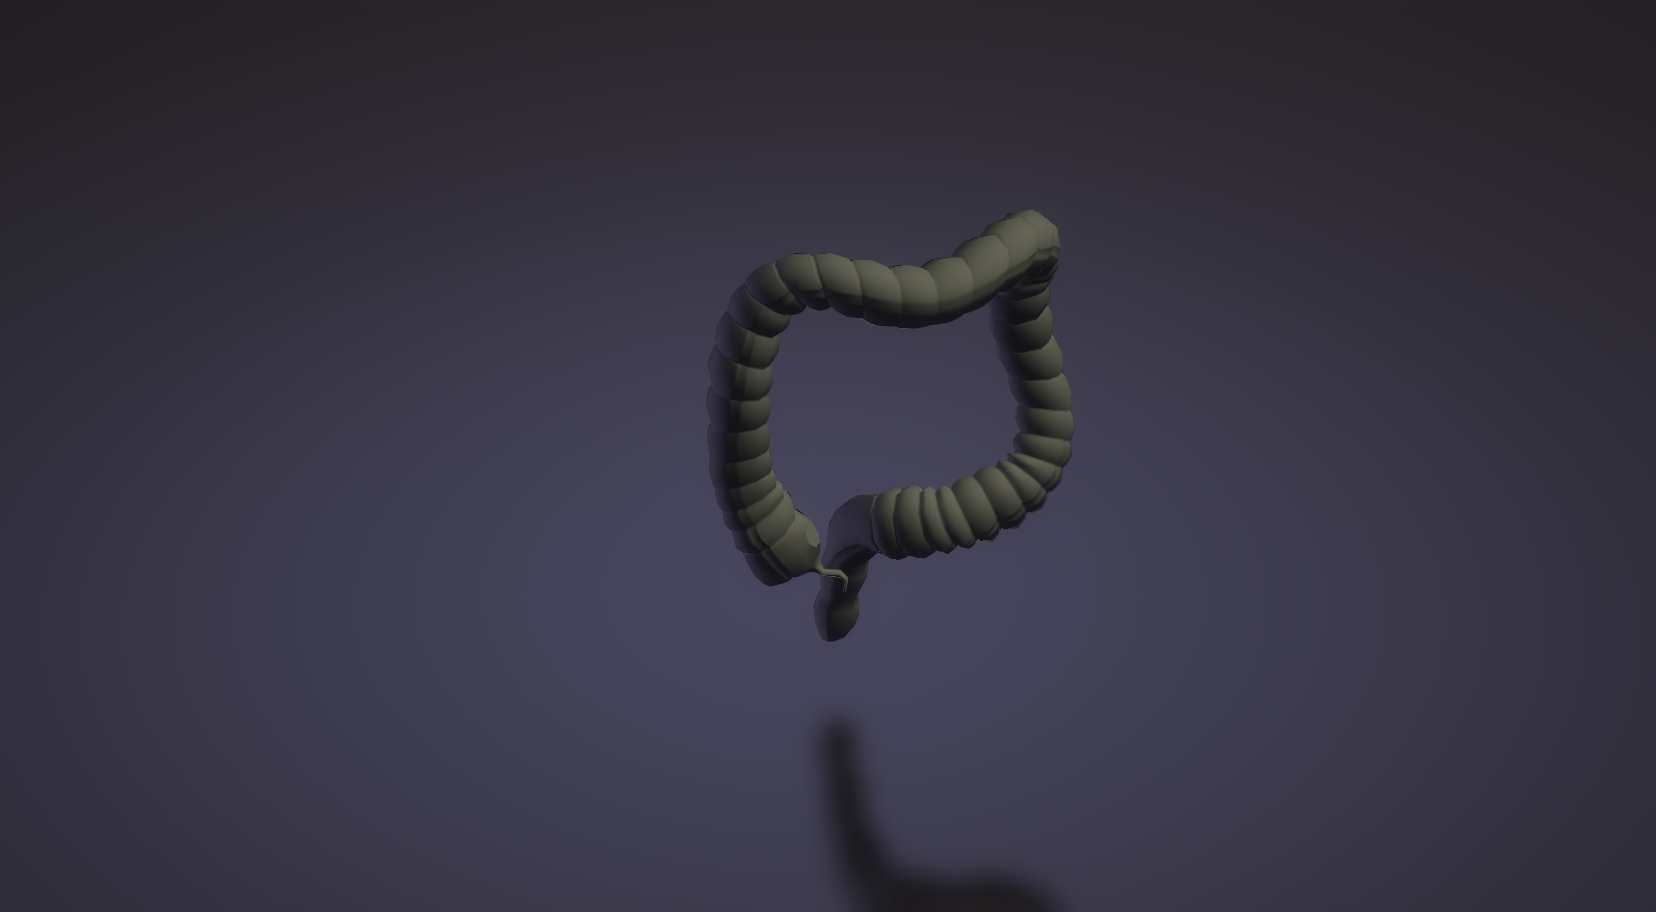
\includegraphics[width = .5\textwidth]{source/images/image20.png}
 		\captionof{figure}{\label{fig:im313}Modelo 3D del intestino grueso}
	\end{center} 
\end{figure}

\section{Modelo del sistema digestivo unificado}
A continuación se muestran las figuras del resultado final del desarrollo del sistema digestivo en el software de modelado en 3D llamado “Blender”, este fue realizado reuniendo todos los modelos de órganos y elementos individuales creados con anterioridad.\\
\begin{figure}[H]
	\begin{center}
 		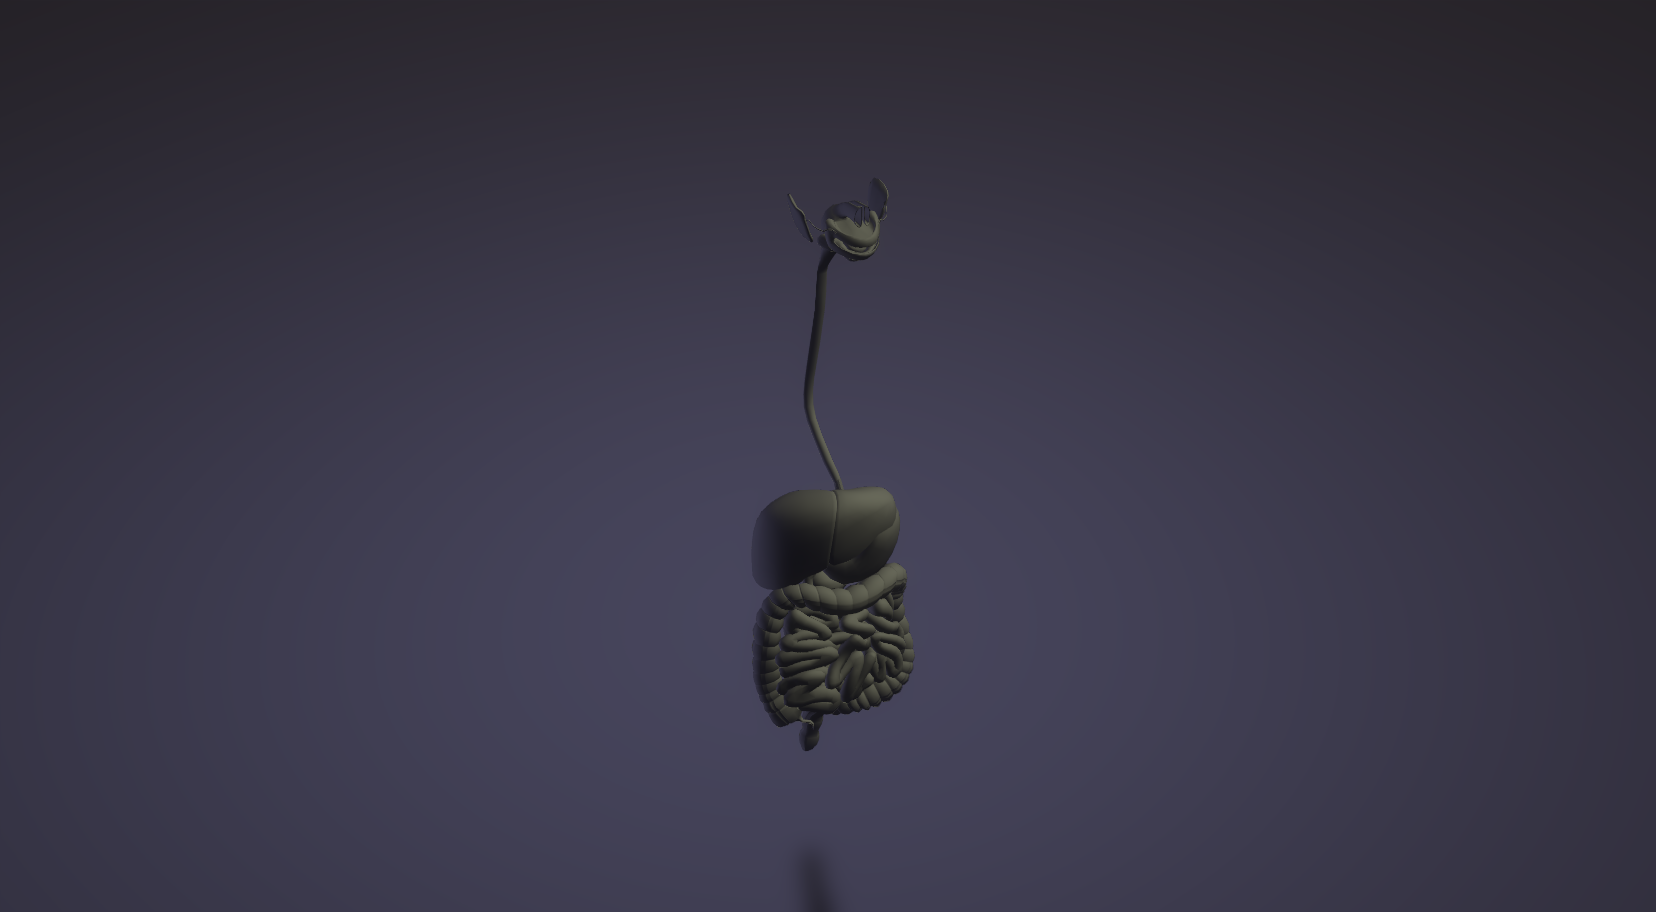
\includegraphics[width = 1\textwidth]{source/images/image24.png}
 		\captionof{figure}{\label{fig:im314}Modelo 3D del Sistema digestivo}
	\end{center} 
\end{figure}

\subsection{Generación de interacción con modelos 3D}
Para poder importar los modelos del sistema digestivo del cuerpo humano estos son agregados dentro de la misma carpeta del proyecto y seleccionar nuevo Asset.\\
Posteriormente estos se agregan a la escena principal del sistema, dependiendo de cuales son los que se deseen integrar.\\
Duplicando el objeto de escena del modelo 3D deseado y  se vuelve a pintar debajo del objeto Meshes en la jerarquía Interactable.Primary\_.Grab.Secondary\_.swap object y 
se ponga a cero los valores de transformación cuando sea necesario.\\
Se inhabilitó el objeto de escena original del modelo 3D deseado.\\
Si es necesario se ajusta la nueva transformación del modelo en 3D en los grados necesarios en el eje Y y se ajusta la transformación Interactable.Primary\_.Grab.Secondary 
swap object para ubicarse en el entorno 3D correctamente.\\
De esta manera se integran rápidamente los elementos multimedia diseñados anteriormente.\\
\begin{figure}[H]
	\begin{center}
 		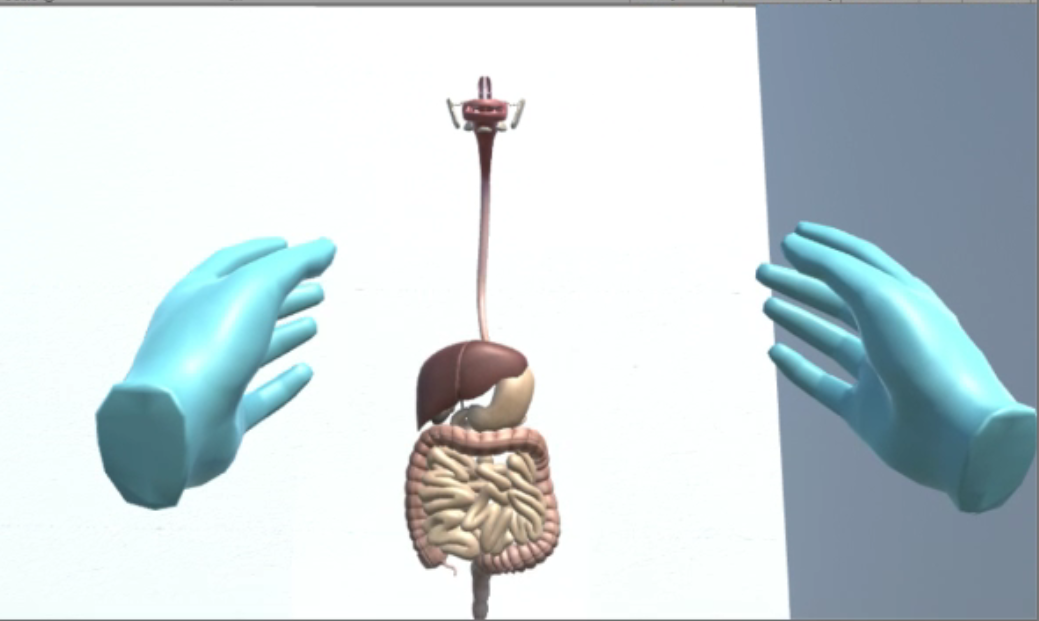
\includegraphics[width = .5\textwidth]{source/images/image37.png}
 		\captionof{figure}{\label{fig:im328}Integración de modelo del sistema digestivo 3D dentro del entorno 3D}
	\end{center} 
\end{figure}
\begin{figure}[H]
	\begin{center}
 		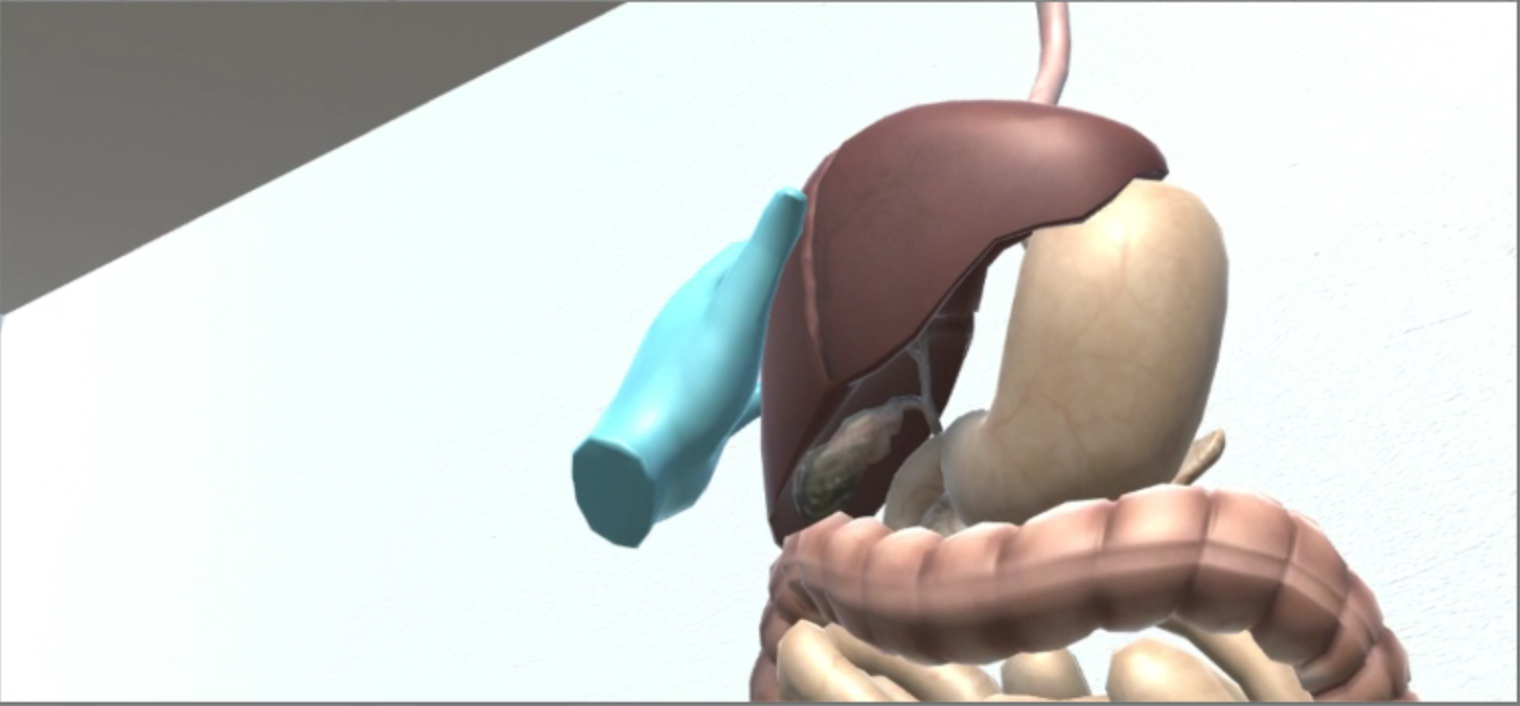
\includegraphics[width = .5\textwidth]{source/images/image67.png}
 		\captionof{figure}{\label{fig:im329}-  Interacción con modelo del hígado del sistema digestivo 3D dentro del entorno 3D}
	\end{center} 
\end{figure}

\section{Evaluación de modelos 3D por personal calificado}
Debido al tiempo de desarrollo, el cual tomó más de lo planteado, de los modelos antes expuestos en la sección anterior no fue posible concretar una cita 
para su evaluación con el personal calificado  de la Escuela Superior de Medicina en las fechas previamente planteadas.\\
Se esperaba poder tener una reunión en fechas posteriores pero la situación epidémica que se ha desarrollado en el país y 
limitaciones impuestas por las autoridades hicieron imposible la evaluación de los modelos desarrollados.\\
Esto no significa que no se haya hecho bajo rigor alguno, sólo se utilizaron materiales de medicina impresos, así como 
referencias en video de disecciones del sistema digestivo, esto para estar lo más familiarizado posible, como estudiante 
de ingeniería en sistemas computacionales, al momento de desarrollar dichos modelos.\\

\section{Diseño y Desarrollo de Componentes de Software}
Los componentes de software a diseñar y desarrollar el cual interactúa con el entorno en 3D y  modelos 3D.\\
Hubo puntos clave desarrollados los cuales tuvieron que ser desarrollada para llevar a cabo la mejor UX. Los desarrollos son incrementales, en cuanto a el grado de interacción 
que se logra.\\
Los componentes desarrollados para este software son:\\
\begin{itemize}
  \item Seguimiento de HMD y controles
  \item Locomoción y ergonomía
  \begin{itemize}
    \item Teleportación
    \item Puntos de teleportación
    \item Giros rápidos, entradas personalizadas, oclusión del usuario    
  \end{itemize}
  \item Presencia e interacción de las manos  
  \begin{itemize}
    \item Agregar manos
    \item Interactuando con entorno
    \item Interacciones manuales adicionales    
  \end{itemize}
\end{itemize}
Todos estos componentes forman la base para que la experiencia del software de realidad virtual se “sienta” lo más “natural” posible y estos mismos deben de estar refinados para que 
al integrarse con los componentes multimedia la interacción con estos se lleve de manera fluida.

\section{Creando el proyecto en Unity ®}
Se optó por el uso de Unity ® en su versión 2018.4 14f1 LTS  ya que esta misma será soportada por más tiempo y es ideal para un desarrollo en el cual se necesite solamente usar una versión estable del editor sin que haya cambios dentro de este que perjudique el desarrollo del sistema; así mismo es la versión que Oculus\cite{web15} recomienda dentro de sus requerimientos y recomendaciones de desarrollo.\\
\begin{figure}[H]
	\begin{center}
 		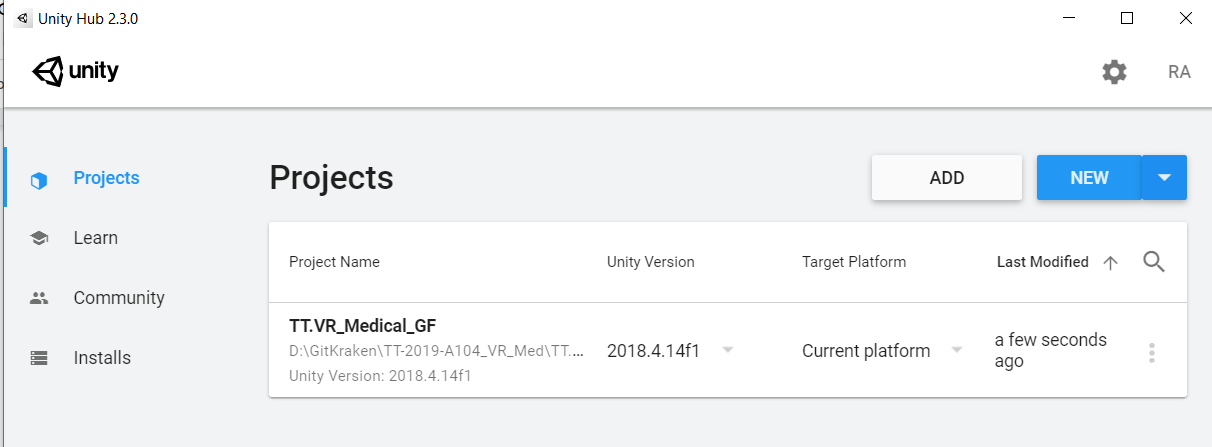
\includegraphics[width = 1\textwidth]{source/images/image51.png}
 		\captionof{figure}{\label{fig:im315}Unity Hub 2.3.0}
	\end{center} 
\end{figure}

\section{Seguimiento de HMD y controles}
En este apartado se realizó en rastreo del HMD y de los controles y que estos se vean reflejados como movimientos dentro del software y replicados en el mismo HMD el cual está 
siendo usado por el usuario y así puede percibir el movimiento. Esto es la base para que el software provea una experiencia en la cual el usuario pueda estar inmerso.\\
Utilizando el SDK que provee Oculus para su desarrollo con el motor Unity se realiza el elemento OVRCameraRig y TrackedAlias.\\
Se abrió el prefabricado OVRCameraRig , así como el objeto secundario TrackingSpace en la jerarquía. Se selecciona OVRCameraRig y luego se navega hasta el script 
LinkedAliasAssociationCollection en el inspector. Se adaptan los siguientes activos en las entradas apropiadas en el Script LinkedAliasAssociationCollection:\\
\begin{itemize}
    \item TrackingSpace a Play Area
    \item CenterEyeAnchor a el HMD
    \item CenterEyeAnchor a la cámara del HMD
    \item LeftHand Anchor al controlador izquierdo
    \item RightHandAnchor al controlador derecho
\end{itemize}
Realizando estos pasos se logra el rastreo de los controles y el HMD ejemplificando con la figura \ref{fig:im315.}.
\begin{figure}[H]
	\begin{center}
 		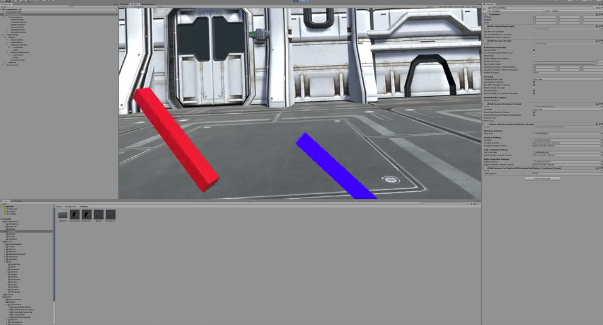
\includegraphics[width = .7\textwidth]{source/images/image44.png}
 		\captionof{figure}{\label{fig:im315.}Entorno de desarrollo Unity mostrando en rastreo del HMD y controles}
	\end{center} 
\end{figure}

\section{Locomoción y ergonomía}
El modo más simple de locomoción es el movimiento físico y este es el más confortable que se puede tener debido a que cuando uno decide moverse en la realidad el 
usuario también se moverá dentro del entorno virtual, pero este viene con limitaciones inherentes y retos que no son plenamente obvios al momento de la concepción y 
desarrollo, se exponen algunos a continuación .\\
\begin{itemize}
    \item Los usuarios poseen áreas de interacción de diferentes tamaños, no todos poseen un área grande lo cual les permite más libertad de movimiento, mientras más pequeño sea el espacio que requiera el usuario más usuarios podrán hacer uso del sistema. Se podría ajustar el contenido del sistema, pero esto implicaría mayor trabajo y tiempo, esto no se traduce en una experiencia de usuario mejor que si este se hubiera diseñado con un área de interacción pequeña en primer lugar.
    \item Se toma en cuenta que con el movimiento físico es probable que algunos usuarios no tengan la posibilidad de moverse físicamente dentro de su área, pueden estar limitados por una discapacidad, lo cual implicaría en que el movimiento sería una distracción para el usuario asumiendo que de algún modo este pudiera interactuar de alguna manera.
\end{itemize}
Otros dos tipos más de locomoción que se consideraron para el desarrollo del sistema uno de estos es el movimiento guionizado y movimiento de avatar, el primero se 
refiere a cuando la perspectiva se mueve a través de un camino predeterminado, este es usualmente utilizado cuando se realiza una experiencia que no requiera movimientos 
del usuario, fácilmente ejemplificado por un viaje en una montaña rusa en un software de realidad virtual este puede llegar a causar vección, generalmente este tipo de 
movimiento suele ser poco tolerable en largos periodos de tiempo.\\
Por otro lado el movimiento de avatar es el clásico movimiento que solemos encontrar en videojuegos o en experiencias pasadas de realidad virtual, al mover una palanca 
del mando el avatar comenzará su movimiento. Este fue un acercamiento más que válido pero con el progreso de la tecnología la manera de implementar el movimiento ha evolucionado.\\
La teleportación se refiere a una mecánica instantánea o casi instantánea en la cual el usuario aparece en un lugar seleccionado, típicamente funciona apuntando hacia al 
lugar deseado y presionando un botón, aunque hay múltiples variaciones de este acercamiento.\\
La teleportación ocurre en un instante lo cual reduce a un mínimo la posibilidad de generar una molestia comparación de los tipos de movimiento expuestos anteriormente.\\
Tomando en cuenta los tipos de movimiento pasado, sus deficiencias y beneficios se tomó la decisión de implementar la teleportación como método de movimiento en el entorno 
virtual del sistema.\\

\subsection{Teleportación}
En este apartado se desarrollaron los movimientos que el usuario pudiera tener dentro del entorno en 3D, estos dan la posibilidad de “movimiento” dentro del mismo así 
como las limitaciones que se implementan para que el mismo usuario no pueda acceder a partes que no queramos o estén disponibles para este.\\
El desarrollo se realizó de la manera siguiente:\\ 
Se cambió el nombre del Prefab a una convención de nombres, en este caso Teleport.Curved. respectivamente, y se realizó una copia para la mano derecha para tener 
un objeto distinto para la mano derecha.\\
Se configuró el script de fachada de puntero adjunto a cada objeto arrastrando el Alias de controlador correspondiente de la Jerarquía al campo FollowSource.\\
Se crearon dos nuevos GameObjects vacíos para el manejo de las entradas del control y adjunto el script OVRInputTouchAction a cada uno de ellos.\\
Se estableció el valor de la propiedad táctil de ambos scripts OVRInputTouchAction en Thumbstick primario. Estableciendo el valor de la propiedad del controlador en L Touch
 y R Touch respectivamente.\\

\begin{verbatim}
    using System.Collections;
using System.Collections.Generic;
using UnityEngine;
using Zinnia.Action;
 
public class OVRInputTouchAction : BooleanAction
{
    public OVRInput.Controller controller = OVRInput.Controller.Active;
    public OVRInput.Touch touch;
 
    void Update() {
        Receive(OVRInput.Get(touch, controller));
    }
}
\end{verbatim}
Para cada objeto de ObjectPointer.Curved, se le asigna el objeto TeleportCurved correspondiente de la Jerarquía con un script OVRInputTouch al campo Acción de activación en el componente Fachada de puntero.\\

De esta manera al tocar cualquier thumbstick este invocará una curva la cual nos mostrará dónde será la teleportación una vez esta sea implementada.\\
\begin{figure}[H]
	\begin{center}
 		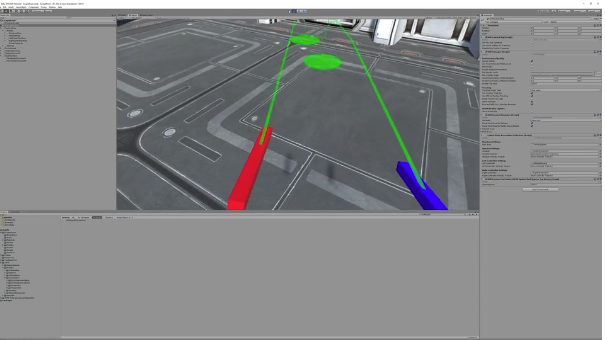
\includegraphics[width = .5\textwidth]{source/images/image73.png}
 		\captionof{figure}{\label{fig:im316}Curva que muestra la ubicación de la teleportación al tocar los thumbstick de los controles.}
	\end{center} 
\end{figure}

Para la adición de la acción de teleportación, la cual es la que permitirá el movimiento del usuario dentro del entorno de realidad virtual. Se tuvo la opción de 
implementar dos tipos de acciones de teleportación, Teleport.Instant y Teleport.Dash, se eligió la primera ya que supone una menor probabilidad de causar vección en el usuario 
 a que no se percibe movimiento alguno en la acción de teleportación.\\
Se implementó VRTK/Locomotion/Teleporter y arrastrando el Teleporter.Prefab instantánea a la escena.\\
%En el script de TeleporterFacade se adjunto al objeto Teleporter.Instant, asignado al objeto de  la escena PlayAreaAlias ​​al campo Target y el objeto de escena HeadsetAlias ​​al campo Offset.\\
Se estableció el campo de validez de la cámara del script de TeleporterFacade en el objeto de escena SceneCameras.\\
Se crearon dos nuevos GameObjects vacíos  para adjuntar las entradas de los botones y se adjunto el script OVRInputButtonAction a cada uno de ellos.\\
Se estableció el valor de la propiedad táctil de ambos scripts OVRInputButtonAction en Thumbstick primario. Se estableció el valor de la propiedad del controlador en 
L.Touch y R.Touch respectivamente.\\

\begin{verbatim}
    using System.Collections.Generic;
using UnityEngine;
using Zinnia.Action;
 
public class OVRInputButtonAction : BooleanAction {
    public OVRInput.Controller controller = OVRInput.Controller.Active;
    public OVRInput.Button button;
 
    void Update() {
        Receive(OVRInput.Get(button, controller));
    }
}
\end{verbatim}

Para cada objeto prefabricado Curva de puntero de objeto, se asignó los GameObjects correspondientes con el script OVRInputButtonAction al campo Acción de selección en el 
componente Fachada de puntero.\\
Para cada puntero de ObjectPointer.Curved, se agregó un nuevo objeto EventData en la lista Datos de acción seleccionados.\\
Se asignó el objeto Teleporter.Instant al campo de objeto ubicando y seleccionando TeleporterFacade y luego Teleport.\\
Implementando los procesos pasados se logra que el usuario pueda teleportarse dentro del  entorno virtual.\\
De esta manera al tocar cualquier thumbstick este invocará una curva la cual nos mostrará dónde será la teleportación una vez esta sea implementada.\\
\begin{figure}[H]
	\begin{center}
 		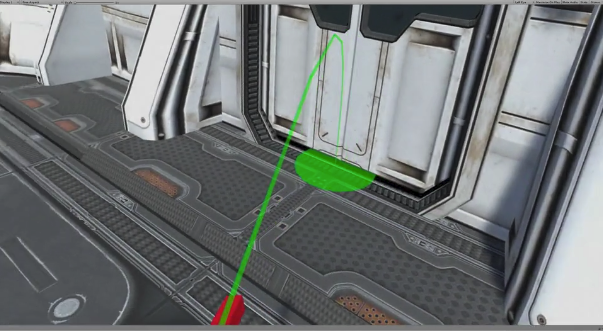
\includegraphics[width = .5\textwidth]{source/images/image35.png}
 		\captionof{figure}{\label{fig:im317}Curva que muestra la ubicación de la teleportación al tocar los thumbstick del control izquierdo.}
	\end{center} 
\end{figure}
\begin{figure}[H]
	\begin{center}
 		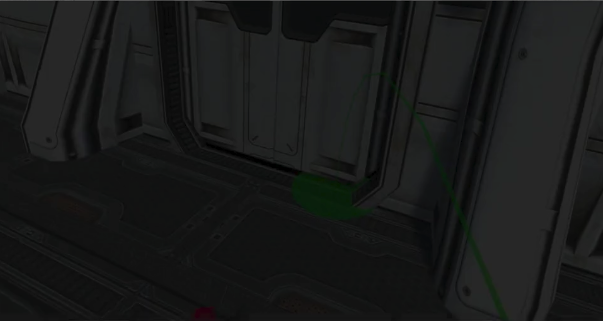
\includegraphics[width = .5\textwidth]{source/images/image61.png}
 		\captionof{figure}{\label{fig:im318}Curva que muestra la ubicación de la teleportación al tocar los thumbstick de los controles.}
	\end{center} 
\end{figure}

En la figura \ref{fig:im318} se puede notar un oscurecimiento, el cual es representativo del desvanecimiento que se implementó para reducir la vección del usuario y evitar 
cinetosis en los usuarios que pudieran llegar a ser propensos a ella.\\
Se procedió a integrar un indicador de flecha el cual servirá para indicar a de cara a que posición se estará cuando se realice la teleportación, así ampliando las posibilidades 
de interacción del usuario y facilitando las mismas.\\
Se importó un modelo de flecha en la vista Proyecto y fue arrastrado a la escena debajo del objeto de escena ValidContainer ubicado dentro de la jerarquía de objetos de escena 
de Destino para cada prefab ObjectPointerCurved.\\
Se ajustó la transformación del nuevo objeto de flecha para que sea visible dentro de la escena y asigne material PointerDefaultValid al renderizador de malla.\\
Se crearon dos nuevos GameObjects para cada control y obtener la dirección del stick del control vacíos y integró el script OVRInputAxis2DAction a cada uno de ellos.\\
Se estableció el valor de la propiedad táctil de ambos scripts OVRInputAxis2DAction en el control primario así como el valor de la propiedad del controlador en L Touch 
y R Touch respectivamente.\\
Se implementa el prefabricado AxisRotator a la escena.\\
Se cambia el nombre del Prefab a una convención de nombres AxisRotator.L  y se realiza una copia para la mano derecha ya se que implemento de la misma manera con el nombre AxisRotator.R\\
Se crearon dos nuevos GameObjects vacíos debajo de cada uno de los objetos OVRInputAxis2DAction creados anteriormente y se agrego el script Vector2ToFloat a los cuatro.\\

\begin{verbatim}
    using System.Collections;
using System.Collections.Generic;
using UnityEngine;
using Zinnia.Action;
 
public class OVRInputAxis2DAction : Vector2Action
{
    public OVRInput.Controller controller = OVRInput.Controller.Active;
    public OVRInput.Axis2D axis;
 
    void Update() {
        Receive(OVRInput.Get(axis, controller));
    }
}
\end{verbatim}

Se estableció el valor del eje del script Vector2ToFloat en el eje correcto, en este caso, una X y una Y para cada objeto OVRInputAxis2DAction.\\
En cada secuencia de comandos OVRInputAxis2DAction, se agregaron dos nuevos objetos Vector2 a la lista de valores cambiados de Vector2.\\
Se asignaron los objetos Vector2ToFloat a cada campo. Usando el menú desplegable, seleccione Vector2ToFloat y luego DoTransform.\\
Use el botón "Agregar componente" en el Inspector para agregar el componente de script FloatAction a cada objeto Vector2ToFloat.\\
En cada scriptVector2ToFloat, agregue un nuevo objeto de acción individual a la lista de acciones individuales transformadas y asigne el objeto primario.\\
Usando el menú desplegable, seleccione FloatAction y luego Recibir.\\
Se configuró cada objeto AxisRotator asignando un objeto FloatAction en los campos Eje lateral lateral y Eje longitudinal correspondientes en el script AxisRotatorFacade 
para los ejes X e Y de cada mano, respectivamente.\\
%En cada script AxisRotatorFacade, se asignó el objeto de escena ValidContainer correspondiente que se encuentra en la Jerarquía de cada prefabricado ObjectPointerCurved al campo Destino. Se asignó el objeto HeadsetAlias ​​al campo Offset direccional en cada uno de los scripts de AxisRotatorFacade.
En la secuencia de comandos de TeleporterFacade, establezca el valor de Uso de desplazamiento en Offset siempre con rotación de destino.\\
Implementando esto se logra que un puntero aparezca en una flecha en la dirección indicada para que el usuario pueda elegir su dirección de orientación al 
elegir la ubicación de teleportación como se muestra en la figura \ref{fig:im319}.\\

\begin{figure}[H]
	\begin{center}
 		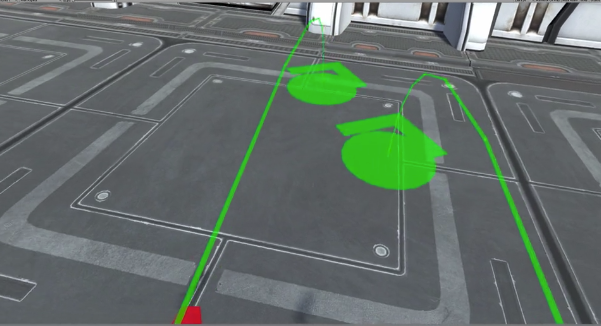
\includegraphics[width = .5\textwidth]{source/images/image62.png}
 		\captionof{figure}{\label{fig:im319}Curva que muestra la ubicación de la teleportación y posición del stick al interactuar con los thumbstick de los controles}
	\end{center} 
\end{figure}
\begin{figure}[H]
	\begin{center}
 		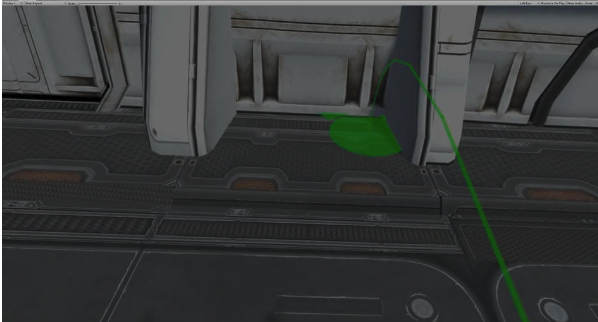
\includegraphics[width = .5\textwidth]{source/images/image4.png}
 		\captionof{figure}{\label{fig:im320}Curva que muestra la ubicación de la teleportación y posición del stick al interactuar con los thumbstick de los controles}
	\end{center} 
\end{figure}

\subsection{Puntos de teleportación}
Los puntos de teleportación son los cuales resaltan una locación dentro del entorno virtual la cual se quiere o requiere que el usuario vaya con facilidad hacia ellas.\\
Se agregó una nueva capa llamada "Teleportable" y se estableció el objeto FloorCollider en la nueva capa.\\
Se creó un nuevo GameObject vacío y se agregaron componente en el Inspector para adjuntar el script AnyLayerRule.\\
Se estableció el campo LayerMask en el script AnyLayerRule en la capa Teleportable.\\
\begin{verbatim}
    namespace VRTK.Prefabs.Locomotion.DestinationLocations
{
    using UnityEngine;
    using UnityEngine.Events;
    using Malimbe.MemberChangeMethod;
    using Malimbe.MemberClearanceMethod;
    using Malimbe.XmlDocumentationAttribute;
    using Malimbe.PropertySerializationAttribute;
    using Zinnia.Rule;
    using Zinnia.Data.Attribute;
 
    /// <summary>
    /// The public interface into the DestinationLocation Prefab.
    /// </summary>
    public class DestinationLocationFacade : MonoBehaviour
    {
        #region Location Settings
        /// <summary>
        /// Determines if the location is in the locked and unusable state.
        /// </summary>
        [Serialized]
        [field: Header("Location Settings"), DocumentedByXml]
        public bool IsLocked { get; set; }
        /// <summary>
        /// Whether to apply the rotation of the custom destination location to the selected action output.
        /// </summary>
        [Serialized]
        [field: DocumentedByXml]
        public bool ApplyDestinationRotation { get; set; } = true;
        /// <summary>
        /// Allows to optionally determine which <see cref="SurfaceData"/> sources can affect the location.
        /// </summary>
        [Serialized, Cleared]
        [field: DocumentedByXml]
        public RuleContainer SourceValidity { get; set; }
        #endregion
 
        #region Location Events
        /// <summary>
        /// Emitted when the Destination Location is entered for the first time.
        /// </summary>
        [Header("Location Events"), DocumentedByXml]
        public UnityEvent HoverActivated = new UnityEvent();
        /// <summary>
        /// Emitted when the Destination Location is entered.
        /// </summary>
        [DocumentedByXml]
        public DestinationLocation.SurfaceDataUnityEvent Entered = new DestinationLocation.SurfaceDataUnityEvent();
        /// <summary>
        /// Emitted when the Destination Location is exited.
        /// </summary>
        [DocumentedByXml]
        public DestinationLocation.SurfaceDataUnityEvent Exited = new DestinationLocation.SurfaceDataUnityEvent();
        /// <summary>
        /// Emitted when the Destination Location is exited for the last time.
        /// </summary>
        [DocumentedByXml]
        public UnityEvent HoverDeactivated = new UnityEvent();
        /// <summary>
        /// Emitted when the Destination Location is activated.
        /// </summary>
        [DocumentedByXml]
        public DestinationLocation.TransformDataUnityEvent Activated = new DestinationLocation.TransformDataUnityEvent();
        /// <summary>
        /// Emitted when the Destination Location is deactivated.
        /// </summary>
        [DocumentedByXml]
        public UnityEvent Deactivated = new UnityEvent();
        #endregion
 
        #region Reference Settings
        /// <summary>
        /// The linked Internal Setup.
        /// </summary>
        [Serialized, Cleared]
        [field: Header("Reference Settings"), DocumentedByXml, Restricted]
        public DestinationLocationConfigurator Configuration { get; protected set; }
        #endregion
 
        /// <summary>
        /// Called after <see cref="IsLocked"/> has been changed.
        /// </summary>
        [CalledAfterChangeOf(nameof(IsLocked))]
        protected virtual void OnAfterIsLockedChange()
        {
            Configuration.SetLockedState(IsLocked);
        }
 
        /// <summary>
        /// Called after <see cref="ApplyDestinationRotation"/> has been changed.
        /// </summary>
        [CalledAfterChangeOf(nameof(ApplyDestinationRotation))]
        protected virtual void OnAfterApplyDestinationRotationChange()
        {
            Configuration.LocationController.ApplyDestinationRotation = ApplyDestinationRotation;
        }
 
        /// <summary>
        /// Called after <see cref="SourceValidity"/> has been changed.
        /// </summary>
        [CalledAfterChangeOf(nameof(SourceValidity))]
        protected virtual void OnAfterSourceValidityChange()
        {
            Configuration.LocationController.SourceValidity = SourceValidity;
        }
    }
}
\end{verbatim}
Se estableció el campo TargetValidity en el script TeleporterFacade en AnyLayerRule script gameobject.\\

Para cada ObjectPointerCurved, se asigno AnyLayerRule al campo TargetValidity del script PointerFacade.\\
\begin{figure}[H]
	\begin{center}
 		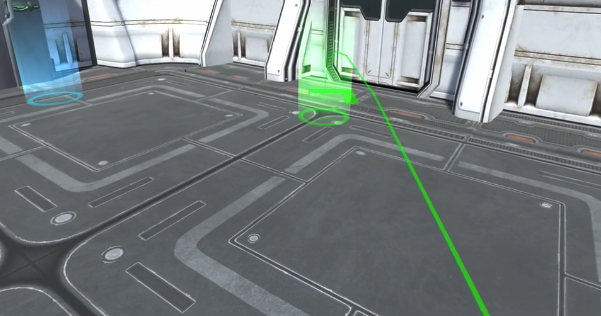
\includegraphics[width = .5\textwidth]{source/images/image45.png}
 		\captionof{figure}{\label{fig:im321}Desvanecimiento al realizar la teleportación y posición del stick al interactuar con los thumbstick del control}
	\end{center} 
\end{figure}

\subsection{Giros rápidos, entradas personalizadas, oclusión del usuario}
En esta sección se implementan giros de la cámara para facilitar al usuario la interacción en el entorno virtual así como la personalización y mejoras de interacción 
con los controles las cuales pretenden hacer más intuitivo el movimiento del usuario en el sistema de realidad virtual, además se implementan oclusiones en determinados 
lugares para evitar que el mismo usuario pueda ver a través de modelos 3D no deseados mermando así la experiencia de usuario.\\
Se creó un nuevo GameObject vacío para obtener  cuando el stick es tocado y adjunto el script de TeleporterActivation y configurando el campo Controlador en R Touch.\\
Se creó otro nuevo GameObject vacío y adjunto la secuencia de comandos TeleporterSelection y configuro el campo Controlador en R Touch.\\ 
Se crearon dos nuevos GameObjects vacíos para ser agregados al InputHandler bajo el script TeleporterSelection GameObject y  adjuntó el script FloatAction a cada uno.\\
Se agregó el componente en el Inspector para agregar los objetos del juego de script FloatAction a los campos Extraer X e Extraer Y del script TeleporterSelection.\\
Se asignaron los campos Eje lateral y Eje longitudinal en la secuencia de comandos AxisRotatorFacade a las dos nuevas secuencias de comandos de FloatAction GameObjects.\\
Fueron deshabilitados los objetos de juego de script OVRInputTouch, OVRInputButtonAction y OVRIInputAxis2DAction para la mano derecha.\\
Fueron reasignados los campos Acción de activación y Acción de selección en la secuencia de comandos de PointerFacade de la derecha a la secuencia de comandos 
TeleporterActivation y TeleporterSelection GameObjects, respectivamente.\\
Se inhabilitó el prefabricado ObjectPointerCurved de la izquierda en la escena y el script OVRInputTouch, OVRInputButtonAction GameObjects para la mano izquierda.\\
\begin{figure}[H]
	\begin{center}
 		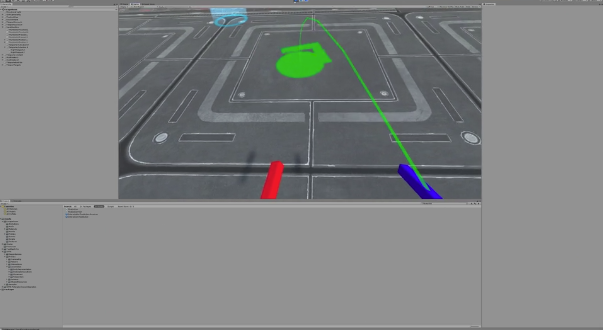
\includegraphics[width = .5\textwidth]{source/images/image57.png}
 		\captionof{figure}{\label{fig:im322} Curva de teleportación habilitada solamente para el control derecho}
	\end{center} 
\end{figure}

En el script AxesToVector3Facade adjunto al PrefabObject, estableciendo el Tipo de uso del eje Direccional.\\
Se  estableció el campo Eje lateral en el valor del eje X FloatAction script GameObject ubicado debajo de la mano izquierda OVRInputAxis2DAction script GameObject.\\
Se estableció el valor del campo Multiplicador de velocidad lateral en 45 y el valor del campo Multiplicador de velocidad longitudinal en 0.\\
Agregando una secuencia de comandos Vector3Cache a la secuencia de comandos AxesToVector3Facade GameObject.\\
Se agregó una nueva acción Vector3 a la lista de acciones Vector3 procesadas en el script AxesToVector3Facade y fueron agregadas al GameObject padre. 
Estableciendo las funciones en Vector3Cache/CachedData.\\
Fue agregado un script CameraColorOverlay al script GameObject de AxesToVector3Facade.\\
Se agregó un nuevo Vector3 a la lista de Vector3 modificado en el script Vector3Cache y  se agrego el objeto del juego principal. Estableciendo las funciones en CameraColorOverlay/link.\\
En el script CameraColorOverlay, se asignó el objeto de escena SceneCameras al campo Validez de la cámara.\\
Se implementó el material de TeleportFade en el proyecto y asignando al campo Material de superposición en el script CameraColorOverlay y cambie el valor del campo Eliminar duración a 0.5.\\
Se creó un nuevo GameObject vacío y se agrego el componente para agregar el script Vector3ToVector2 y un script Vector2ToVector3.\\
Fue agregada una nueva acción Vector3 a la lista de acciones Vector3 procesadas en el script AxesToVector3Facade y agregando el GameObject del script Vector3ToVector2. Se estableció la 
función en Vector3ToVector2/DoTransform.\\
Se agregó una nueva acción Vector2 a la lista de acciones Transform(Vector2) en el script Vector3ToVector2 y agregó el GameObject principal. Se establecieron las funciones en 
Vector2ToVector3\/.DoTransform.\\
Se establecieron dentro del campo Mapa de coordenadas en X a Y e Y a X excluyendo Z en el script Vector3ToVector2. Se agregó el script TransformEulerRotationMutator al objeto de 
juego de script Vector3ToVector2.\\
En el script Vector2ToVector3, fue agregada una nueva acción Vector3 a la lista de acciones Transform(Vector3). Asignando el GameObject principal y estableciendo el menú 
desplegable en TransformEulerRotationMutator/DoIncrementProperty.\\
Estableciendo el campo Destino en el script TransformEulerRotationMutator para el objeto de escena PlayAreaAlias. Se activan las opciones usar valores locales y mutar en el eje Y 
e inhabilitar las opciones mutar en el eje X y mutar en el eje Z.\\
\begin{figure}[H]
	\begin{center}
 		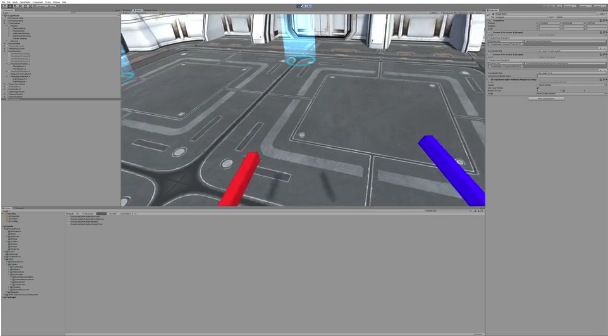
\includegraphics[width = .5\textwidth]{source/images/image47.png}
 		\captionof{figure}{\label{fig:im323} Captura previa de giro rápido con stick de control izquierdo}
	\end{center} 
\end{figure}
\begin{figure}[H]
	\begin{center}
 		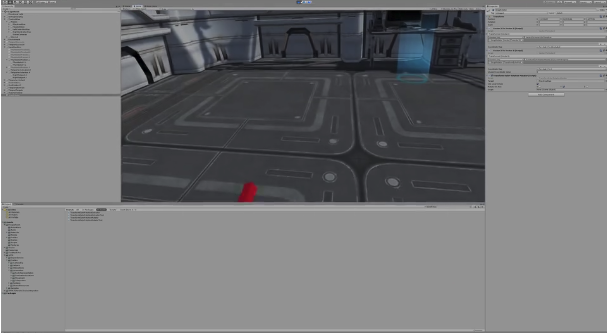
\includegraphics[width = .5\textwidth]{source/images/image71.png}
 		\captionof{figure}{\label{fig:im324}Captura posterior de giro rápido con stick de control izquierdo}
	\end{center} 
\end{figure}
Deshabilitando el objeto SnapToFloor debajo del objeto Teleporter\_.InstantPrefab en la escena.\\
Utilizando el prefabricado CollisionFader en el proyecto y arrastrándolo a la escena debajo del objeto de escena HeadsetAlias.\\
En el script CameraColorOverlay adjunto al prefabricado CollisionFader, se estableció el campo CameraValidity en el objeto de escena SceneCameras.\\
Fueron creadas dos nuevas capas llamadas FadeCamera y FadeOut. Colocando el objeto prefabricado CollisionFader en la capa FadeCamera.\\
Se colocó el objeto de la escena principal en la capa FadeOut. Se cambió la matriz de colisión para que la capa FadeCamera solo colisione con la capa FadeOut.\\
Cambiando el valor del campo ClearFlags en los scripts de la cámara bajo el GameObject de escena OVRCameraRig a color sólido y configurando el color en negro.\\

\section{Presencia e interacción de las manos}
Desde la introducción de los controles Oculus Touch para el sistema Oculus Rift y similares, la presencia de las manos ha sido la manera principal de proveer una experiencia de 
realidad virtual, los usuarios pueden encontrar manos virtuales que simulan las que poseen en realidad, esto nos ayuda a utilizar el conocimiento de los usuarios del mundo real y 
trasladarlo a el entorno virtual en lugar de tener que crear y asignar botones y crear controles complicados ya que las manos en la realidad virtual son tan importantes como en 
la realidad.\\
La implementación de manos en el sistema de realidad virtual se realizó de la manera siguiente:\\

\subsection{Agregar manos}
Se integraron los prefabricados CustomHandLeft y CustomHandRight en el proyecto y se adicionaron a  los prefabricados LeftControllerAlias y RightControllerAlias 
correspondientes en la escena.\\
Deshabilitando el script OVRGrabber en los objetos de escena CustomHandLeft y CustomHandRight.\\
Deshabilite el componente MeshRenderer para los objetos Cube en las jerarquías LeftControllerAlias y RightControllerAlias.\\
Se establecieron la capa de los objetos de escena CustomHandLeft y CustomHandRight para ignorar Raycast.\\
\begin{figure}[H]
	\begin{center}
 		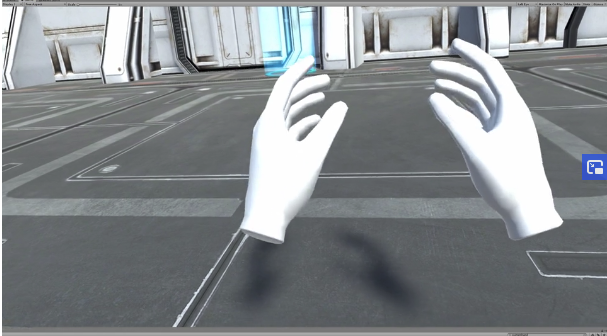
\includegraphics[width = .5\textwidth]{source/images/image74.png}
 		\captionof{figure}{\label{fig:im325}Cambio de placeholders por modelos de manos en 3D}
	\end{center} 
\end{figure}
Un método de configuración y refinamiento de la posición de las manos es utilizando el  HMD y se compara la posición de sus manos reales con la de las manos virtuales, otro método que se utilizó fue cambiar los modelos dentro del entorno mediante prueba y error, comprobando qué tan similar es la localización de los dedos conforme a la realidad comparada a lo que se ve en el entorno virtual.\\
\begin{figure}[H]
	\begin{center}
 		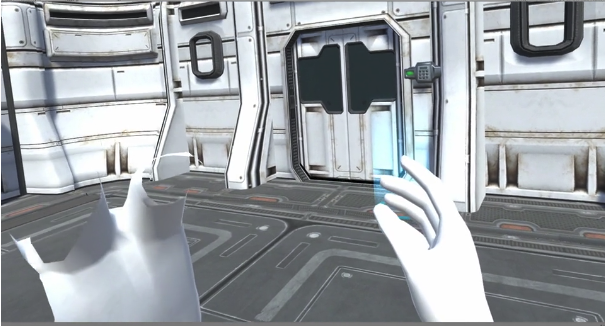
\includegraphics[width = .5\textwidth]{source/images/image48.png}
 		\captionof{figure}{\label{fig:im326}Oclusión deshabilitada para modelo de manos 3D}
	\end{center} 
\end{figure}
\begin{figure}[H]
	\begin{center}
 		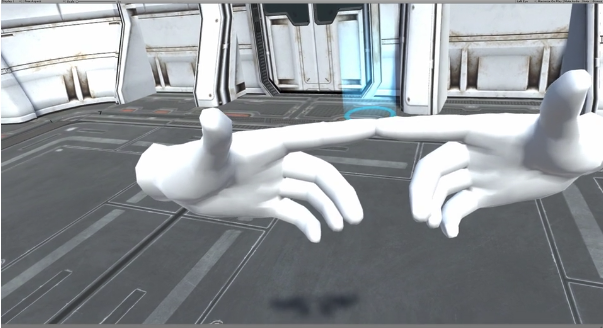
\includegraphics[width = .5\textwidth]{source/images/image23.png}
 		\captionof{figure}{\label{fig:im327}Refinado de localización de manos en el entorno virtual}
	\end{center} 
\end{figure}
Cabe mencionar que debido a la diferencia de complexión de los humanos no se puede realizar una configuración universal de estos elementos.\\
Se localizan los modelos OculusTouchRift\_.Left y OculusTouchRift\_.Right ubicados en la  escena LeftControllerAlias y RightControllerAlias respectivamente para hacer una 
representación del control en el entorno virtual, si se decide utilizarse en un futuro.\\

\subsection{Interactuando con entorno}
%Se implementa el prefab de Interactor en el proyecto y se agrega uno debajo de los prefab LeftControllerAlias ​​y RightControllerAlias ​​en la escena.
Se inhabilitó el MeshRenderer en el objeto ExampleAvatar en cada una de las jerarquías de objetos de Interactor.\\
Creando dos nuevos GameObjects para agregarlo al InputHandler y poder controlar los gatillos posteriormente y se agrega el componente en el inspector para agregar los scripts
OVRInputAxis1DAction y FloatToBoolean a cada objeto.\\
En los scripts FloatToBoolean, se establezca el campo límites positivos entre 0,75 y 1. Esto para tener una sensación de agarre conforme se va presionando el botón y no sea 
cuando ya está presionado completamente el gatillo.\\
En cada secuencia de comandos OVRInputAxis1DAction, se establezca el campo controlador en los valores L Touch y R Touch correspondientes y establezca el campo axis en 
Disparador manual primario. Se agrega componente en el inspector para agregar el script BooleanAction a cada objeto.\\
En los scripts OVRInputAxis1DAction, se agregó un nuevo objeto de acción individual en la lista de acciones individuales de ValueChanged. Agregando el GameObject principal 
y se estableció el script en FloatToBoolean/DoTransform.\\
En los scripts FloatToBoolean, se agregó un nuevo objeto de acción booleana en la lista de acciones booleanas transformadas. Agregando el GameObject principal y estableciendo 
en BooleanAction/Receive.\\
En los scripts de InteractorFacade en los prefabricados de Interactor en la escena, estableciendo el campo GrabAction en los GameObjects de script BooleanAction correspondientes.\\
Se utiliza el prefab Interactable.Primary\_.Grab.Secondary Swap en el proyecto y se agregó debajo de la jerarquía de objetos de escena y se hizo coincidir su transformación para 
los valores de transformación del objeto de escena del modelo en 3D con el cual se quiere interactuar.\\
Se deshabilitó el objeto DefaultMesh en la jerarquía Interactable.Primary\_.Grab.Secondary swap object.\\
Duplicando el objeto de escena del modelo 3D deseado y  se vuelve a pintar debajo del objeto Meshes en la jerarquía Interactable.Primary\_.Grab.Secondary\_.swap object y 
se ponga a cero los valores de transformación cuando sea necesario.\\
Se inhabilitó el objeto de escena original del modelo 3D deseado.\\
Si es necesario se ajusta la nueva transformación del modelo en 3D en los grados necesarios en el eje Y y se ajusta la transformación Interactable.Primary\_.Grab.Secondary 
swap object para ubicarse en el entorno 3D correctamente.\\

\subsection{Interacciones manuales adicionales}

Para dar una sensación de inmersión más fidedigna se integran los siguientes elementos, estos harán que la gravedad y la velocidad que es impuesta a un objeto se mantenga.\\
Se agregó el script OVRAnchorVelocityEstimator a los objetos de escena LeftHandAnchor, RightHandAnchor y CenterEyeAnchor.\\
En cada script OVRAnchorVelocityEstimator fue establecido el campo Tracked GameObject en el objeto padre del juego y el campo Relative To en el objeto de la escena TrackingSpace.\\
En el script LinkedAliasAssociationCollection adjunto al objeto de escena OVRCameraRig, establezca el campo Headset Velocity Tracker en el objeto de escena CenterEyeAnchor, 
el campo Left Controller Velocity Tracker en el objeto de escena LeftHandAnchor y el campo en el objeto de escena RightHandAnchor.\\
%Para cada prefab del interactor, se estableció el campo VelocityTracker del script InteractorFacade en el LeftControllerAlias ​​y RightControllerAlias ​​correspondientes.\\

\section{Integración de componentes del producto}
Para el integración de producto, como el mismo nombre de esta fase lo menciona los productos antes realizados, los componentes multimedia y de software finalmente se unen 
dentro del sistema.\\

\chapter{Pruebas Experimentales}

\section{Introduccón}
\chapter{Conlusiones y Trabajo a Futuro}

\section{Introduccón}
\begin{center}
    \chapter{Referencias y Glosario}
\end{center}

    \newpage

\section{Glosario}
\begin{itemize}
 \item \textbf{VR:} Virtual Reality, en español, Realidad Virtual
 \item \textbf{RV:} Realidad Virtual
 \item \textbf{ICs:} Tecnologías de la Información y la Comunicación
 \item \textbf{WIMP:} del inglés window-icon-menu-pointing device
 \item \textbf{MRI:} Imagen por resonancia magnética del inglés Magnetic Resonance Imaging
 \item \textbf{CT:} Computed Tomography del inglés Tomografía axial computarizada
 \item \textbf{PET:} Tomografía por emisión de positrones del inglés Positron Emission Tomography
 \item \textbf{DICOM:} Imagen digital y comunicación sobre medicina. Digital Imaging and Communication On Medicine
 \item \textbf{HMD:} Casco de realidad virtual del inglés Head Mounted Display
 \item \textbf{UML:} Lenguaje de modelado unificado del inglés Unified Modeling Language
 \item \textbf{3D:} Tres Dimensiones del inglés 3 Dimensions
 \item \textbf{I/O:} Entrada y salida del inglés Input/Output
 \item \textbf{UX:} UX (por sus siglas en inglés User eXperience) o en español Experiencia de Usuario, es aquello que una persona percibe al interactuar con un producto o servicio. Logramos una buena UX al enfocarnos en diseñar productos útiles, usables y deseables, lo cual influye en que el usuario se sienta satisfecho, feliz y encantado.
 \item \textbf{VOD:} Del inglés  Video On Demand, El vídeo bajo demanda, o televisión a la carta, es un servicio OTT de televisión. Esta modalidad de difusión de contenidos multimedia, permite al usuario acceder a un contenido concreto, en el momento que lo solicita, visualizandolo en línea en su dispositivo.
 \item \textbf{SDK:} Un kit de desarrollo de software (en inglés, software development kit o SDK) es generalmente un conjunto de herramientas de desarrollo de software que permite a un desarrollador de software crear una aplicación informática para un sistema concreto, por ejemplo ciertos paquetes de software, entornos de trabajo
 \item \textbf{RUP:} El Proceso Unificado de Rational o RUP (por sus siglas en inglés de Rational Unified Process) es un proceso de desarrollo de software desarrollado por la empresa Rational Software, actualmente propiedad de IBM.
\end{itemize}
%\chapter{Introducción}

\section{Introduccón}

Este documento es el reporte técnico final del trabajo terminal titulado 
“Sistema de realidad virtual del cuerpo humano para el estudio del sistema digestivo”
 con número de registro TT: 2019-A104.

En el presente capítulo se habla del problema identificado, 
por qué se considera como tal y cómo es que se ayudó a resolver el problema planteado mediante la 
ingeniería en sistemas computacionales. También se menciona que se obtiene al concluir con este trabajo terminal, tales como el prototipo del sistema.
En el capítulo \textbf{II Análisis} se mostrarán todos los diagramas y documentos generados al analizar y generar un diseño del sistema que se estará desarrollando.\\
 Aquí se encuentra la arquitectura general del sistema, y los modelos gráficos de apoyo presentados en el Análisis Estructurado Moderno.\\
En el capítulo \textbf{III Diseño} se describe el trabajo generado en el desarrollo del documento hasta el mes de mayo de 2020 para TT2.\\
En el capítulo \textbf{IV Verificación y Pruebas} se muestran pruebas hechas sobre las implementaciones del sistema siguiendo un guión para la prueba.\\
En el capítulo \textbf{V Conclusión} se muestran los resultados obtenidos y experiencias para mejorar el proceso, así como la vertiente para continuar con el trabajo
 y las conclusiones del integrante.\\
Finalmente, se encuentran las referencias de todos los recursos empleados para dar soporte y estructura a este Trabajo Terminal, y en los apéndices se anexan elementos
 extra que dan información más detallada sobre lo que aquí fue realizado.\\

\section{Detección del problema} 
Durante 2019 se entrevistó al Dr. Rios Macias jefe del área de morfología de la Escuela Superior de Medicina del Instituto Politécnico Nacional y comentó que “los medios
 que se utilizan para el estudio del cuerpo humano principalmente son medios impresos tradicionales, así como el uso de cuerpos para su disección y análisis posterior”.\\
 El uso de cuerpos para su disección tiene un alto costo que incluye el mantenimiento del cuerpo en las instalaciones, el mantenimiento de las instalaciones, y la inhumación 
 de los cuerpos.
\\
\newline

\section{Propuesta de Solución}
Se elaboró un sistema de realidad virtual del sistema digestivo del cuerpo humano que permite interactuar con modelos tridimensionales. La intención es sentar las bases
 para un sistema de apoyo al aprendizaje que sea más práctico \cite{moore1995learning}, sin sustituir a ningún método de estudio tradicional.
\\
\newline

\section{Justificación}
\label{just}
El sistema tiene los siguientes beneficios para docentes y alumnos: 
\begin{itemize}
\item Fuentes confiables. Se usaron textos médicos y sitios web especializados
\item Uso de realidad virtual\cite{norton1994integrating}.
\end{itemize}
El sistema es un ejemplo de cómo se pueden actualizar las herramientas educativas, como las que se pueden encontrar en Statista \cite{web1},
 y que representan un mercado de aproximadamente 18.8 mil millones de dólares para el año 2020. Además, Nielsen\cite{web2} muestra los datos
  sobre la expectativa de adopción de la realidad virtual y aumentada en diferentes continentes, como se muestra el Figura \ref{fig:graph1} y \ref{fig:graph2}.
\begin{figure}[H]
	\begin{center}
 		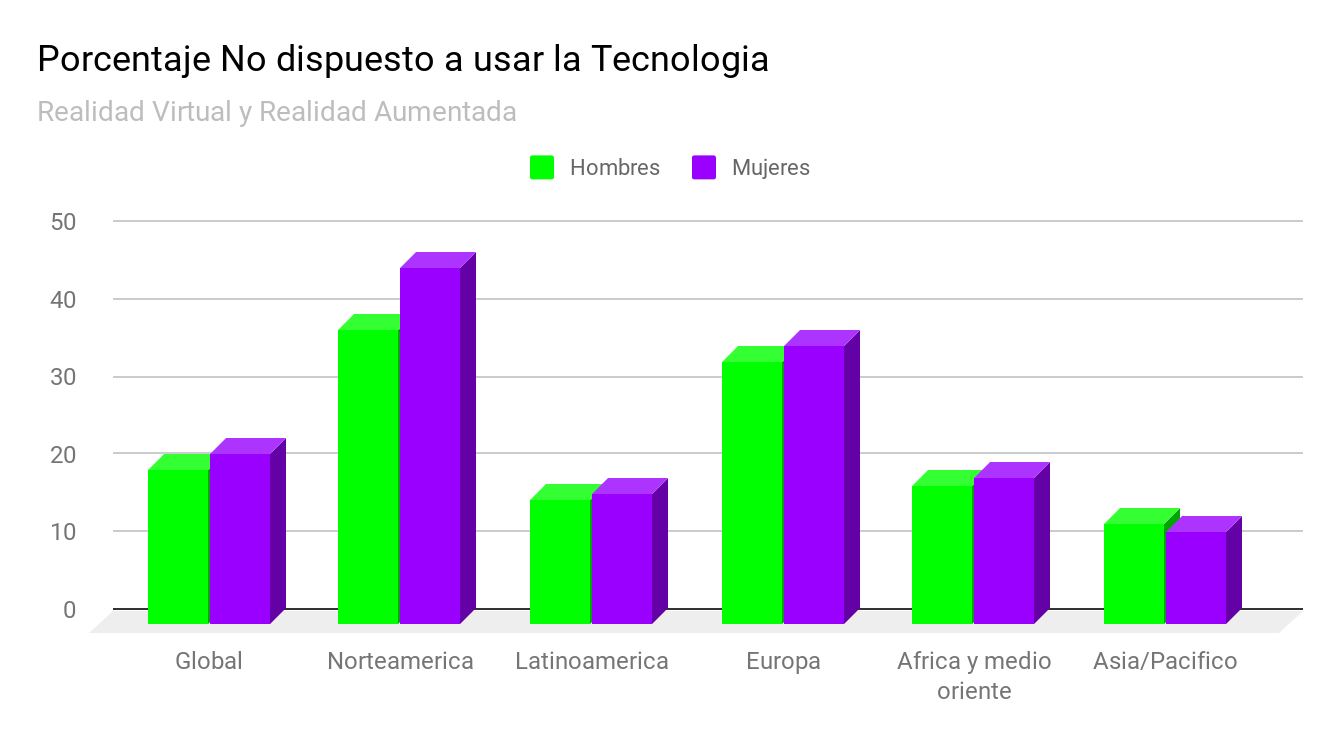
\includegraphics[width = 0.7\textwidth]{source/images/image2.png}
		 \captionof{figure}{\label{fig:graph1}Disposición de los consumidores a nivel mundial para usar la realidad virtual y aumentada si esta se encuentra disponible
		  en los próximos 2 años (2020 -2021)}
	\end{center} 
\end{figure}
\begin{figure}[H]
	\begin{center}
 		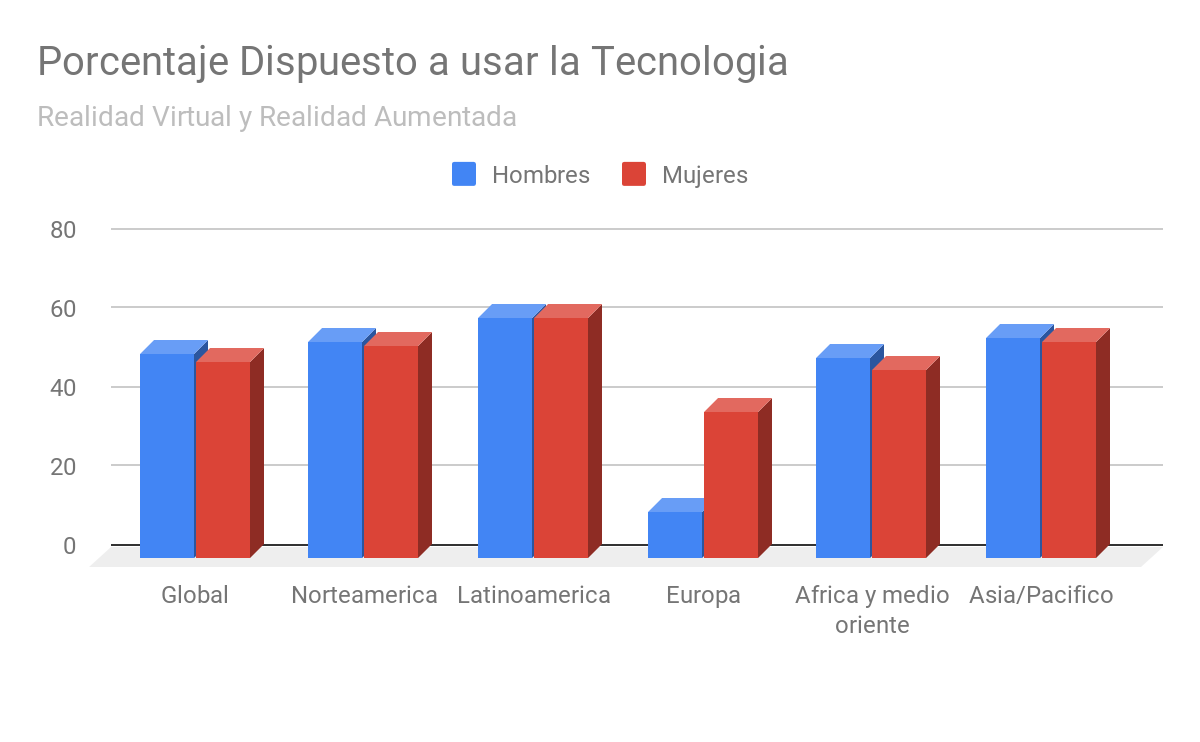
\includegraphics[width = 0.7\textwidth]{source/images/image10.png}
		 \captionof{figure}{\label{fig:graph2}Disposición de los consumidores a nivel mundial para no  usar la realidad virtual y aumentada si esta se encuentra disponible
		  en los próximos 2 años(2020 -2021)}
	\end{center} 
\end{figure}
A medida que crece el consumo de software, multimedia y videojuegos se aumentará la disponibilidad de sistemas como el que se propone en este trabajo terminal.
\\

\section{Objetivos del Trabajo}
Objetivo es analizar, diseñar, desarrollar y probar un sistema de demostración que utiliza la tecnología de Realidad Virtual, para ofrecer una experiencia orientada
 al estudio de la anatomía y morfología del cuerpo humano, específicamente del sistema digestivo.
\newline

\subsection{Objetivos Específicos}
Para lograr el objetivo se identificaron los siguientes objetivos específicos:
\newline
\begin{itemize}
\item Investigar en fuentes confiables sobre el sistema digestivo.
\item Analizar, diseñar, desarrollar y probar un entorno de Realidad Virtual para la interacción.
\end{itemize}

\section{Población Objetivo}
De acuerdo a un estudio de Ericsson ConsumerLabe\cite{web3}, en el año 2020 un tercio de los consumidores serán usuarios de Realidad Virtual. Ya desde 2017 se había
explorado el nivel de interés de los consumidores en Realidad Virtual\cite{web4} con su potencial de reunir gente de todo el mundo y crear un experiencia más profunda,
personalizada y enriquecida.\\
\newline
De todos los interesados en la Realidad Virtual se toma a los estudiantes de educación superior del área de medicina, particularmente a 180\cite{ofi1}  estudiantes de
 la Escuela Superior de Medicina del Instituto Politécnico Nacional de entre 18 y 24 años de edad. Además se espera que los usuarios objetivo tengan las siguientes 
 características\cite{web5} específicamente:\\
\newline
\begin{itemize}
\item Disposición para el aprendizaje con nuevas tecnologías de la información.
\item Conocimientos sólidos en las áreas de biología, física, química; y en forma idónea conocimientos básicos de las etimologías grecolatinas e idioma inglés, que le 
facilitarán la comprensión y dominio de los conceptos utilizados en las asignaturas básicas y clínicas.
\item No ser propenso a sufrir cinetosis.
\end{itemize}

\section{Productos logrados}
Se logró crear un software (demostración), de una experiencia demostrativa en realidad virtual. El sistema muestra características y elementos del sistema digestivo y 
permite la participación de un usuario utilizando una misma computadora de forma local. Se usan los controles Oculus Touch ® así como el visor de Realidad Virtual Oculus 
Rift ®. También se redactó el presente reporte técnico.

\section{Definiciones}
Estas son las definiciones más importantes para el presente trabajo terminal

\subsection{Realidad Virtual}
Algunos autores definen así la Realidad Virtual.\\
\newline
\textit{“La realidad virtual (RV) es una simulación tridimensional generada o asistida comúnmente por computadora de algún aspecto del mundo real o ficticio, en el cual 
el usuario tiene la sensación de pertenecer a ese ambiente sintético o interactuar con él”}\cite{web6}\\ 
\textbf{Corrado Padila Érica}\\
\newline
“Realidad Virtual: gráficos 3D en entornos inmersivos que usan I/O
artefactos como guantes, cascos, etc. en busca de mayores grados de iteración
con el ambiente virtual”\cite{web7}\\ 
Lozano Miguel, Calderón\\
\newline
"Realidad Virtual es una forma en que los seres humanos puedan
visualizar, manipular e interactuar con las computadoras y datos extremadamente
complejos".\cite{web8}\\
Isdale, Jerry\\
\newline
“Un sistema interactivo capaz de crear una simulación que implique a varios de los sentidos del ser humano, generados por una computadora, explorable, visualizable y manipulable 
en tiempo real; este bajo la forma de imágenes y sonidos, estos, dando la sensación de presencia en el entorno generado”\cite{web9}\\
Levis, Diego\\
\newline
Esta última ha sido la definición que se ha tomado para el desarrollo del proyecto del trabajo terminal, asimismo se puede concluir que todos los autores coinciden en que la 
realidad virtual es un mundo simulado en el que el usuario puede interactuar en tiempo real por medio
de dispositivos o computadoras que logran un efecto artificial e inmersivo en el que se pueden manipular objetos.

\subsection{Producto Multimedia}
Los productos multimedia se pueden clasificar en dos categorías: productos interactivos y no interactivos. Los productos no interactivos también se pueden clasificar en 
productos estáticos como carteles, logotipos, folletos, modelos estáticos 3D, etc., y productos basados en el tiempo. \cite{engels2002object,sauer2001uml}.\\ 
\newline
Los productos multimedia interactivos son aplicaciones de software que contienen productos multimedia\cite{miranda2017diseno} (es decir, aplicaciones basadas en eventos 
como juegos, aplicaciones web basadas en multimedia y materiales de aprendizaje multimedia basados en interactividad).  La figura \ref{fig:diag1} a continuación ilustra 
los tipos de productos multimedia.\\
\begin{figure}[H]
	\begin{center}
 		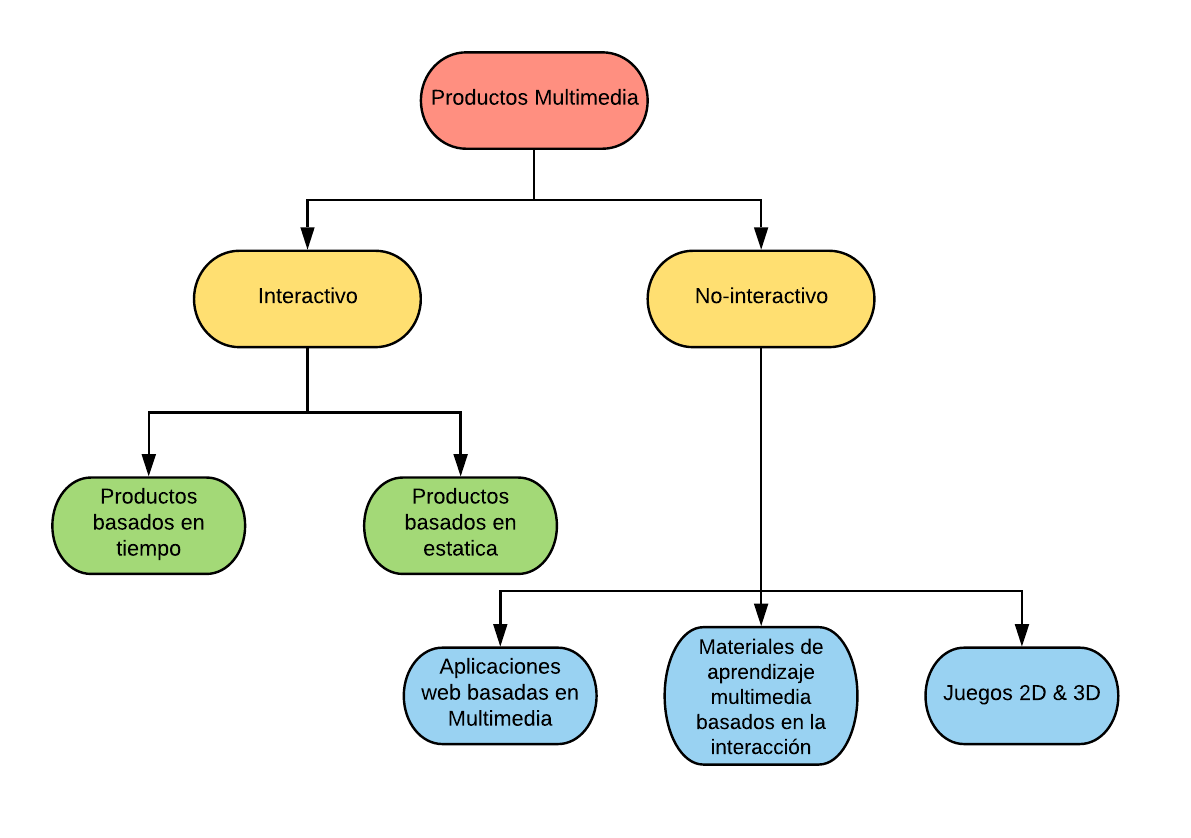
\includegraphics[width = 1\textwidth]{source/images/image52.png}
 		\captionof{figure}{\label{fig:diag1}Tipos de productos multimedia} 
	\end{center} 
\end{figure}

Un sistema multimedia se puede analizar desde tres puntos:
\begin{itemize}
\item La vista externa. La forma en que el usuario interactúa con el producto.
\item Flujo de acciones. El orden en que se muestran los marcos de los modelos a los usuarios. \cite{aleem2016game,cartwright1996pre}.
\item  Los roles de los usuarios. La interacción con productos multimedia.
\end{itemize} 
El cuadro \ref{tab:tab1} resume los tipos de productos multimedia y sus características.

\begin{longtable}[c]{
>{\columncolor[HTML]{EFEFEF}}c ccc}
\cellcolor[HTML]{C0C0C0} &
  \multicolumn{3}{c}{\cellcolor[HTML]{C0C0C0}\textbf{Características Multimedia}} \\
\multirow{-2}{*}{\cellcolor[HTML]{C0C0C0}\textbf{\begin{tabular}[c]{@{}c@{}}Tipos de productos\\  multimedia\end{tabular}}} &
  \cellcolor[HTML]{C0C0C0}\textbf{\begin{tabular}[c]{@{}c@{}}Vista \\ \\ Externa\end{tabular}} &
  \cellcolor[HTML]{C0C0C0}\textbf{\begin{tabular}[c]{@{}c@{}}Flujo \\ \\ de acciones\end{tabular}} &
  \cellcolor[HTML]{C0C0C0}\textbf{\begin{tabular}[c]{@{}c@{}}Roles de \\ \\ los Usuarios\end{tabular}} \\
\endfirsthead
%
\endhead
%
\hline
\endfoot
%
\endlastfoot
%
\textit{Productos estáticos} &
  Un cuadro &
  Sin acciones &
  Pasivo (ver/leer) \\
\textit{\begin{tabular}[c]{@{}c@{}}Productos basados\\  en tiempo\end{tabular}} &
  Múltiples cuadros &
  Secuencia &
  Pasivo(mirar) \\
\textit{Productos interactivos} &
  Impulsado por eventos &
  \begin{tabular}[c]{@{}c@{}}Secuencia, Selectiva,\\  Interactiva e\\  Impulsada por eventos\end{tabular} &
  Activo(Realiza eventos) \\ \hline
\caption{Características de los productos multimedia.}
\label{tab:tab1}\\
\end{longtable}
Para este trabajo, el sistema que se propone es una producto interactivo.

\section{Estado del Arte}
A continuación se muestran algunos de trabajos académicos desarrollados en México y fueron comparados con el trabajo planeado. Como comparativa y de forma ilustrativa 
del sector académico.\\
\newline
\begin{enumerate}
\item TT No. 2014-A058 “Sistema para la orientación de los efectos sobre la espalda humana en pacientes con sobrepeso”\cite{tt1}
\item TT No. 2012-B055 “Laboratorio Virtual del cuerpo humano 3D con asistente de ayuda en línea para el nivel superior bajo el paradigma de Educación Basada en Web con 
tecnologías de Web Semántica”\cite{tt2}
\item TT No. 2014-B035 “Simulación en Tercera Dimensión del Sistema Circulatorio de los Cánidos para el uso Educativo”\cite{tt3}
\item TT No. 2014-B039 “Simulación de una Línea del Metro con Realidad Virtual”\cite{tt4}
\item Tesis que para optar por el grado de Maestro en Ciencia e Ingeniería de la Computación, Sistema de seguimiento de movimiento de las extremidades superiores basado 
en sensores inerciales para rehabilitación en realidad virtual.\cite{mastersthesis1}
\item Adecuación educativa de la realidad virtual como herramienta didáctica para el proceso enseñanza-aprendizaje / tesis que para obtener el título de Licenciado en 
Pedagogía, presenta Maria de la O García Noriega; asesor Lucina Moreno Valle Suárez.\cite{te1}
\end{enumerate}
Así mismo se ha encontrado software propietario desarrollado por empresas privadas los cuales son los siguientes.\\
\begin{itemize}
\item The Body VR: Anatomy Viewer es la única herramienta de visualización de Realidad Virtual disponible en el mercado que se basa en datos médicos específicos del 
paciente (por ejemplo, MRI, CT, PET) y cumple con los estándares DICOM. Proporciona simulaciones de R.V. anatómicas en tiempo real para visualizar diagnósticos médicos, 
ilustrar el impacto de los procedimientos y tratamientos, y crear una toma de decisiones más educada.\
\begin{figure}[H]
	\begin{center}
 		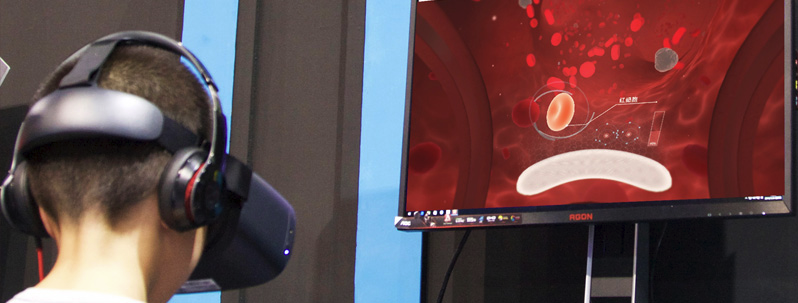
\includegraphics[width = 0.5\textwidth]{source/images/image9.png}
 		\captionof{figure}{\label{fig:ea1}Software “The Body VR” en uso.}
	\end{center} 
\end{figure}
\item Anatomyou VR: Estructuras anatómicas fotorrealistas, modeladas en colaboración con RenderArea, validadas por expertos clínicos y certificadas por personal capacitado 
en  Tecnologías Médicas de la Universidad de Las Palmas de Gran Canaria.
\begin{figure}[H]
	\begin{center}
 		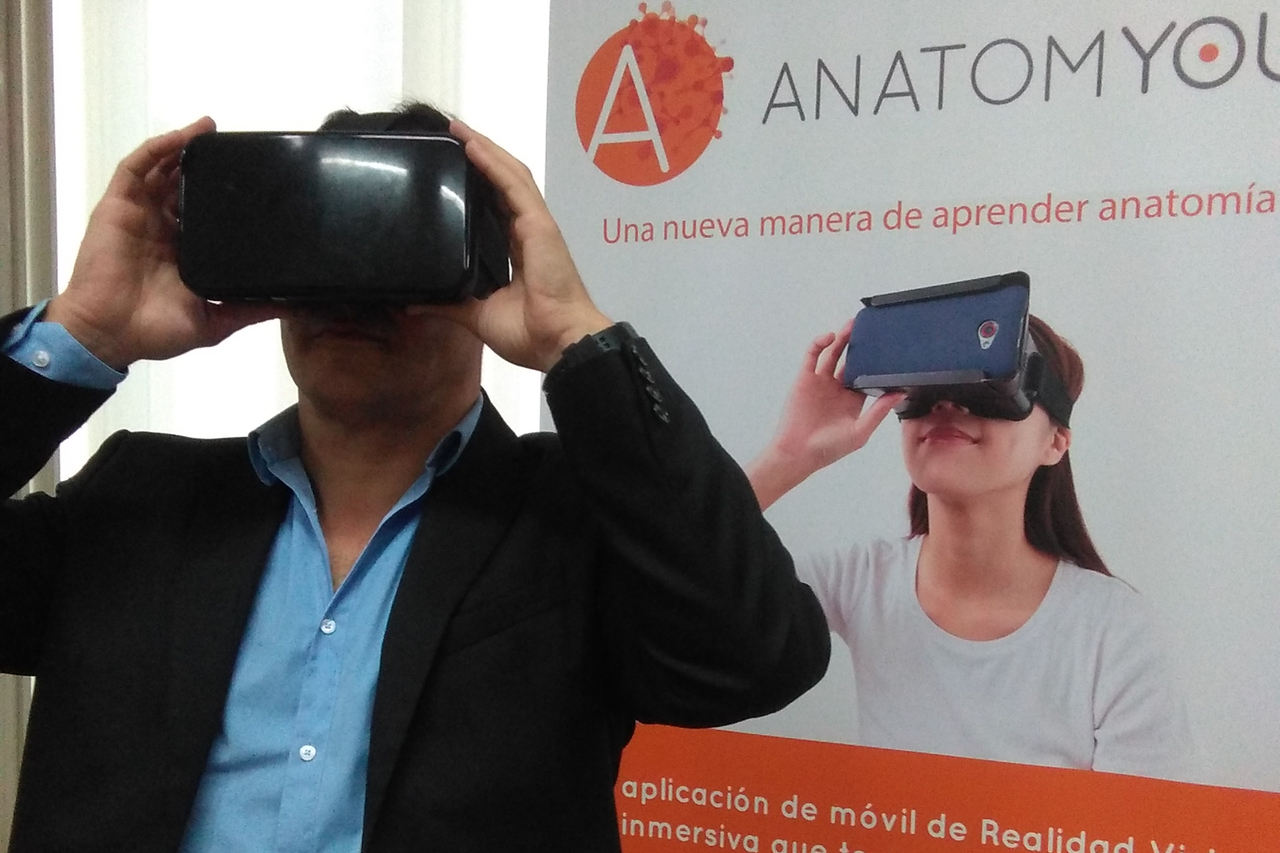
\includegraphics[width = 0.5\textwidth]{source/images/image59.png}
 		\captionof{figure}{\label{fig:ea2}Pancarta promocional de “Anatomyou VR}
	\end{center} 
\end{figure}
\item Biodigital Anatomy: El cuerpo tridimensional más completo, científicamente preciso e interactivo jamás ensamblado. Anatomía masculina y femenina, en los detalles 
básicos (gratuitos) y profesionales. Cada sistema está completamente segmentado, etiquetado y direccionable para una fácil configuración que satisfaga cualquier necesidad educativa.
\begin{figure}[H]
	\begin{center}
 		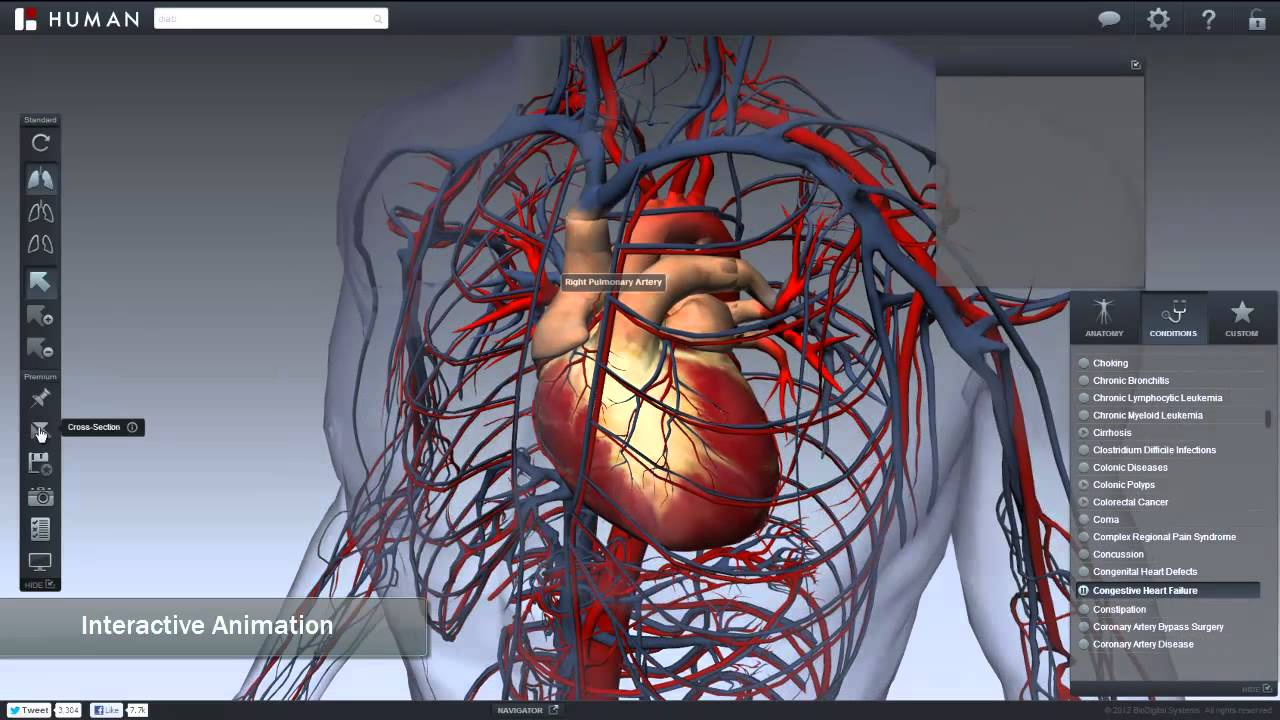
\includegraphics[width = 0.5\textwidth]{source/images/image18.png}
 		\captionof{figure}{\label{fig:ea3}Interfaz del software de Biodigital Anatomy}
	\end{center} 
\end{figure}
\item 3D Organon VR Anatom: 3D Organon es un completo atlas anatómico que presenta los 15 sistemas del cuerpo humano. Incluye más de 4,000 estructuras y órganos anatómicos 
realistas y más de 160 correlaciones clínicas encontradas por sistema del cuerpo.
\begin{figure}[H]
	\begin{center}
 		\includegraphics[width = 0.5\textwidth]{source/images/image5.png}
 		\captionof{figure}{\label{fig:ea4}Interfaz del software de 3D organon VR Anatom}
	\end{center} 
\end{figure}
\end{itemize}
%%
%% Este es uno de los puntos más críticados del trabajo,
%% la falta de metodología, así que es donde hay que revisar más.
%% Falta:
%%    - Colocar las referencias a OpenUp y RUP.
%%    - Escribir el acrónimo de RUP.
%%    - Explicar como se adaptó OpenUP
%%    - Mostrar la comparativa de OpenUP vs OpenUP adaptado a este TT.
%%
\section{Metodologías}
Se siguió como modelo de desarrollo a la metodología OpenUp\cite{balduino2007introduction}, 
que está basada en RUP. 
OpenUP es extensible y se usó como base, ya que se adaptó al desarrollo de este proyecto.
La figura \ref{fig:me1} muestra el ciclo de vida iterativo de OpenUP.
\begin{figure}[H]
	\begin{center}
 		\includegraphics[width = 0.5\textwidth]{source/images/image70.png}
 		\captionof{figure}{\label{fig:me1}Ciclo de Vida Iterativo de OpenUP}
	\end{center} 
\end{figure}
OpenUP está organizado en contenido y proceso, con cuatro fases concepción o creación del proyecto, preparación o elaboración detallada del proyecto, construcción y transición.\\
Además también se consideró la Metodología de ingeniería de software multimedia que tiene como fases, requisitos y preproducción, diseño y producción, validación y 
Postproducción y evolución, como se puede ver en la figura \ref{fig:me2}
\begin{figure}[H]
	\begin{center}
 		\includegraphics[width = 1\textwidth]{source/images/image50.png}
 		\captionof{figure}{\label{fig:me2}Fases de la Metodología de ingeniería de software multimedia}
	\end{center} 
\end{figure}
También se tomó como referencia a Git-flow\cite{driessen2010successful} que es un modelo de ramificación que consiste en separar cada característica en su propia rama de desarrollo.
 Se utiliza una versión simplificada del modelo\cite{krusche2014introduction} compuesta por tres tipos principales de ramas.\\
\begin{itemize}
\item \textbf{master:} El código fuente refleja un estado listo para producción.
\item \textbf{develop:} La última entrega con cambios de desarrollo.
\item \textbf{feature:} Nuevas características para el próximo lanzamiento.
\end{itemize}
Otros factores a considerar son que tomando en cuenta el libro Análisis Estructurado Moderno de Edward Yourdon “debe usarse cualquier modelo que se adapte a la situación en la
 que se encuentra.”\cite{edward1989modern}. Aunque la metodología de metodología de ingeniería de software multimedia no propone un diagrama en específico como modelo gráfico para 
 la visualización del proceso general de la realización del sistema de forma general, para este trabajo se considera apropiado emplear diagramas adicionales a manera de tener una 
 mejor visión del proyecto.\\
\begin{itemize}
\item \textbf{Diagramas de Flujo de Datos:}  Estos nos permiten comprender cómo se mueven y procesan los datos en el sistema, visualizando el sistema como una red de procesos.
\item \textbf{Diagramas de Flujo.} Describe gráficamente la lógica de un procedimiento específico.
\end{itemize}

%\begin{figure}[H]
%	\begin{center}
% 		\includegraphics[scale=•]{•} = 0.5\textwidth]{images/ipn.png}
% 		\captionof{figure}{\label{fig:IPN}Descripción de la %imagen} 
%	\end{center} 
%\end{figure}

%\begin{center}
\chapter{An\'alisis}
\end{center}
\newpage

\section{Sistema operativo y platadorma de desarrollo}
EL cuadro \ref{tab:t21} es la comparativa de las plataformas que se analizaron para la elaboración del trabajo terminal.

\begin{table}[H]
\centering
\resizebox{\textwidth}{!}{%
\begin{tabular}{
>{\columncolor[HTML]{C0C0C0}}l lll}
\hline
\multicolumn{4}{c}{\cellcolor[HTML]{9B9B9B}{\color[HTML]{333333} \textbf{Plataforma Windows}}} \\
\multicolumn{1}{c}{\cellcolor[HTML]{9B9B9B}{\color[HTML]{333333} \textbf{Descripción}}} &
  \multicolumn{1}{c}{\cellcolor[HTML]{9B9B9B}{\color[HTML]{333333} \textbf{Software}}} &
  \multicolumn{1}{c}{\cellcolor[HTML]{9B9B9B}{\color[HTML]{333333} \textbf{Costo}}} &
  \multicolumn{1}{c}{\cellcolor[HTML]{9B9B9B}{\color[HTML]{333333} \textbf{Operatividad}}} \\
Sistema Operativo &
  Windows 10 Pro &
  MXN\$5,199.00 &
  \begin{tabular}[c]{@{}l@{}}Ideal para pequeñas empresas o\\  usuarios que necesiten una\\  funcionalidad mejorada.\end{tabular} \\
Sistema Operativo &
  Windows 10 Home &
  MXN\$3,599.00 &
  Ideal para uso personal o doméstico. \\
Sistema Operativo &
  Windows 10 Pro para Workstations &
  MXN\$7,899.00 &
  \begin{tabular}[c]{@{}l@{}}Ideal para los usuarios avanzados y\\  pequeñas empresas que buscan \\ funcionalidad mejorada con la \\ capacidad de calcular cargas de\\  trabajo intensivas.\end{tabular} \\
Sistema Operativo &
  Windows Server 2019 &
  MXN\$10,814.69 &
  \begin{tabular}[c]{@{}l@{}}Sistema operativo que une los entornos\\  on-premises con Azure y agrega capas\\  adicionales de seguridad a la vez que\\  te ayuda a modernizar tus aplicaciones\\  e infraestructura.\end{tabular}
\end{tabular}%
}
\caption{Sistemas operativos de plataforma Windows}
\label{tab:t21}
\end{table}

El cuadro \ref{tab:t22} muestra la comparativa de las plataformas de desarrollo que se analizaron para la elaboración del trabajo terminal.

\begin{table}[H]
\resizebox{\textwidth}{!}{%
\begin{tabular}{|c|c|c|l|}
\hline
\rowcolor[HTML]{9B9B9B} 
\multicolumn{4}{|c|}{\cellcolor[HTML]{9B9B9B}\textbf{Plataforma de desarrollo}}                                                \\ \hline
\rowcolor[HTML]{9B9B9B} 
\textbf{Descripción} & \textbf{Software} & \textbf{Costo} & \multicolumn{1}{c|}{\cellcolor[HTML]{9B9B9B}\textbf{Operatividad}} \\ \hline
\cellcolor[HTML]{C0C0C0}Motor de Desarrollo &
  Unity Free &
  Gratis &
  \begin{tabular}[c]{@{}l@{}}Unity es un motor de videojuego\\  multiplataforma creado por Unity Technologies.\\  Unity está disponible como plataforma de desarrollo\\  para Microsoft Windows, Mac OS, Linux. \\ La plataforma de desarrollo tiene soporte de compilación\\  con diferentes tipos de plataformas\end{tabular} \\ \hline
\cellcolor[HTML]{C0C0C0}Motor de Desarrollo &
  Unreal Engine 4 &
  Gratis &
  \begin{tabular}[c]{@{}l@{}}Unreal Engine es un motor de juego creado por la compañía\\  Epic Games, mostrado inicialmente en el shooter en primera\\  persona Unreal en 1998. \\ Aunque se desarrolló principalmente para los shooters en primera\\  persona, se ha utilizado con éxito en una variedad de otros géneros.\end{tabular} \\ \hline
\end{tabular}%
}
\caption{Plataforma de desarrollo.
}
\label{tab:t22}
\end{table}

Tomando en cuenta la infraestructura que posee la Escuela Superior de Medicina del Instituto Politécnico Nacional, específicamente el Departamento de Computación se optó por usar el sistema operativo Windows 10 Pro y Unity ®.

\section{Hardware}
De acuerdo a las especificaciones del software seleccionado se recomienda usar:\\
\begin{itemize}
\item Tarjeta Gráfica: NVIDIA GTX 1060 / AMD Radeon RX 480 o mejor
\item Tarjeta Gráfica Alternativa: NVIDIA GTX 970 / AMD Radeon R9 290 o mejot
\item CPU: Intel i5-4590 / AMD Ryzen 5 1500X o mejor
\item Memoria: 8GB+ RAM
\item Salida de Video: Compatible HDMI 1.3 video output
\item USB puertos: 3x USB 3.0 y  1x USB 2.0
\end{itemize}
Y en caso de no contar con estos elementos, el mínimo es:
\begin{itemize}
\item Tarjeta Gráfica: NVIDIA GTX 1050Ti / AMD Radeon RX 470 o mejor
\item Tarjeta Gráfica Alternativa: NVIDIA GTX 960 / AMD Radeon R9 290 o mejor
\item CPU: Intel i3-6100 / AMD Ryzen 3 1200, FX4350 o mejor
\item Memoria: 8GB+ RAM
\item Salida de Video: Compatible HDMI 1.3 video output
\item Puertos USB: 1x USB 3.0 y 2x USB 2.0
\end{itemize} 

\section{Viabilidad}
También se analizó la factibilidad del proyecto en general. Desde el punto de vista técnico se realizó una evaluación de la tecnología actual existente y la posibilidad de utilizarla en el desarrollo del sistema. Además de DirectX versión 11 el cuadro \ref{tab:t23} muestra los recursos técnicos necesarios para la ejecución correcta del software:\\
\begin{table}[H]
\centering
\begin{tabular}{|c|c|l|}
\hline
\rowcolor[HTML]{9B9B9B} 
\textbf{Cantidad} &
  \textbf{Recursos} &
  \multicolumn{1}{c|}{\cellcolor[HTML]{9B9B9B}\textbf{Características}} \\ \hline
\cellcolor[HTML]{C0C0C0}1 &
  Computadora Personal de Escritorio &
  \begin{tabular}[c]{@{}l@{}}Tarjeta gráfica discreta, RX480\\ Memoria RAM 16 Gb\\ 5 Puertos USB\\ Procesador de 4 núcleos o mayor\end{tabular} \\ \hline
\cellcolor[HTML]{C0C0C0}1 &
  Sistema de realidad Virtual Oculus Rift &
  \begin{tabular}[c]{@{}l@{}}Visor HMD, controles Touch \\ \\ Sensores Touch.\end{tabular} \\ \hline
\end{tabular}
\caption{ Recursos Técnicos.}
\label{tab:t23}
\end{table}
Económicamente, se determinaron los recursos para desarrollar el sistema así como la comparativa con el uso de cuerpos para su examinación y estudio. Después de un análisis e investigación de los costos con la dirección del Área de Morfología en la Escuela Superior de Medicina bajo la asesoría del Dr. Macias Rios se determinó que el costo que se tiene para el traslado, mantenimiento, uso e inhumación de los cuerpos es de \$40,000.00 c/u, como se ve en el cuadro \ref{tab:t24}.
\begin{center}
\begin{table}[H]
\centering
\begin{tabular}{|
>{\columncolor[HTML]{C0C0C0}}c |l|}
\hline
\multicolumn{2}{|c|}{\cellcolor[HTML]{9B9B9B}\textbf{Costo de uso de cuerpos.}} \\ \hline
Traslado, mantenimiento, uso e inhumación           & \$40,000.00 c/u           \\ \hline
Total                                               & \$40,000.00 c/u           \\ \hline
\end{tabular}
\caption{Costo de cálculo de uso de cuerpos.}
\label{tab:t24}
\end{table}
\end{center}
En el caso del desarrollo e implementación del proyecto se consideró la depreciación, como se observa en el cuadro \ref{tab:t26}.


Para ofrecer una experiencia aceptable al momento del uso del equipo de Realidad Virtual y el software se proponen los elementos del cuadro \ref{tab:t27}.


Además, el sistema de Realidad Virtual con sus componentes tiene un costo que se muestra en el cuadro \ref{tab:t28}.

Se estimaron los suelos de programador y modelado, como se observa en el cuadro \ref{tab:t29}.

Los servicios estimados se muestran en el cuadro \ref{tab:t210} y en el cuadro \ref{tab:t211} se muestra la suma total y como resultado se obtiene el costo total del proyecto, que se estima en: \$326,316.86.

En resumen, el costo de usar nueve cuerpos sería de \$360,000.00 y el del proyecto de \$326,318.00, con lo cual se puede considerar viable económicamente.

\section{Análisis de la plataforma Unity ®}
Unity ® es un motor de desarrollo de videojuegos multiplataforma desarrollado por Unity ® Technologies. Con él se pueden crear videojuegos, simuladores, software de realidad virtual y aumentada. Puede generar código para computadoras de escritorio, portátiles, consolas de videojuegos, Smart TV y otros dispositivos móviles. Ofrece una API de scripting en C\#. En la figura 8 se puede ver el entorno en general.\\

%\begin{center}
\chapter{Diseño}
\end{center}
\newpage

En este capítulo se desarrolla los apartados dedicados a la planeación del trabajo a realizar, comenzando con el diseño utilizando elementos de la metodología de Metodología de ingeniería de software multimedia y los elementos de apoyo de la metodología estructurada de Yourdon cuando estos sean necesarios para ejemplificar diseño o acciones específicas del software. 

\section{Selección de estrategia de diseño}
Con respecto a la realidad virtual, una de las cosas básicas a considerar es la forma en que nuestros sentidos sirven como la entrada que nuestro cerebro utiliza para construir una comprensión del mundo que nos rodea. La vista, el oído, el tacto, el olfato y el gusto son el conjunto de estímulo externo más ampliamente aceptado que percibe el cuerpo humano.\\

Estos sentidos y nuestras reacciones a ellos son el resultado de milenios de selección natural y hay varias consecuencias de esto incorporadas en nuestro instinto. Todo esto es un conocimiento relativamente común y parece que no es necesario reiterar aquí, pero lo importante es afirmar que nosotros, como humanos, tenemos ciertos resultados predecibles basados en ciertos conjuntos de entradas. Esencialmente, es instinto, naturaleza humana.\\

Un sitio web bien diseñado utilizará de manera similar el color, la distancia y la tipografía para comunicar claramente un propósito y, a menudo, persuadir algún tipo de acción.\\

Para que todo esto sea efectivo, se deben implementar y descubrir principios de diseño razonables. Existen varios principios para el diseño que pueden traducirse de otros medios. El diseño de impresión, el diseño web, la arquitectura, el diseño de interiores, el teatro, los gráficos en movimiento, etc., tienen elementos que pueden considerarse relevantes y adoptados.[ 36]\\

Al mismo tiempo, el medio de la realidad virtual como propiedades, como la capacidad de intersección del contenido, son únicas.\\

Es por esto que el diseño de un sistema de realidad virtual presenta retos los cuales son difíciles de sobrellevar ya que se tiene que crear una experiencia para el usuario en el sistema mismo lo cual conlleva a la selección de una estrategia de diseño centrada en la UX del usuario.\\

\section{Requisitos para el desarrollo de software para proveer una experiencia de realidad virtual optima.}
\subsection{Los cuatro núcleos del diseño UX para RV}
Se tomaron en cuenta dos consideraciones centrales para el diseño de experiencias de realidad virtual:
\begin{enumerate}
\item Que fuera interactivo 
\item Que fuera reactivo.
\item Que fuera cómodo
\item Que fuerafácil de usar.
\end{enumerate}

\section{Flexibilidad del Diseño}
La Metodología de ingeniería de software multimedia provee la libertad para elegir el desarrollo de los elementos de “Diseño y desarrollo de componentes multimedia” y “Diseño y desarrollo de componentes de software” y así alternar el desarrollo y diseño de los múltiples elementos que se utilizan dentro del proyecto. Para un documento técnico más ordenado se incluirán primeramente los componentes multimedia y posteriormente los componentes de software aunque estos hayan sido desarrollados en diferentes momentos, como la metodología da la libertad de realizarlo.\\

\section{Componentes multimedia}
En general, independientemente de la disciplina, el proceso de modelado es una simplificación de un objeto para su posterior estudio o representación. Así, podemos hablar de modelos matemáticos que simplifican fenómenos físicos, o modelos meteorológicos para la predicción del tiempo atmosférico, etc. Un modelo geométrico define la información sobre la forma (geometría) de un determinado objeto. Las simplificaciones que se realicen en su definición vendrán determinadas por diferentes factores como el método de representación utilizado, operadores empleados o nivel de detalle.\cite{web13} \\

Se puede definir el proceso de modelado geométrico tridimensional como el encargado de crear modelos consistentes que puedan ser manejados algorítmicamente en un computador. Este proceso de construcción se aborda en diferentes etapas, partiendo típicamente de entidades básicas y aplicando una serie de operadores sobre ellas. Estas entidades básicas pueden ser primitivas geométricas (calculadas de forma algorítmica o mediante una ecuación matemática) u obtenidas mediante un dispositivo de captura (escáner 3D).\\

Existen multitud de técnicas de modelado 3D. En una primera taxonomía de alto nivel podemos hacer una categorización dependiendo de si el modelado se centra en definir únicamente las características del contorno del objeto, los siguiente son los mas usados:\\
\begin{itemize}
\item \textbf{Modelado Sólido:} también conocidos como de Geometría Sólida Constructiva (CSG Constructed Solid Geometry). Los modelos sólidos definen el volumen del objeto que representan, y en muchos casos indican incluso el centro de masas, la densidad del material interna, etc. Se utilizan en fabricación por computador y en aplicaciones médicas e industriales.
\item \textbf{Modelado de Contorno:} también conocidos como de Representación de Contorno (B-Rep - Boundary Representation). Los modelos de contorno únicamente representan la superficie límite del objeto (de forma conceptual, la "cáscara"). Son más fáciles de definir y modificar. Además, lo interesante para la representación del objeto es su apariencia exterior (en los casos donde interesa el interior simplemente se aproxima, como en el caso del SubSurfaceScattering). Prácticamente todos los paquetes de diseño y animación (incluido Blender) empleados en síntesis de imagen y en aplicaciones interactivas emplean este tipo de modelos.
\end{itemize}
Para  cubrir las necesidades de los modelos 3D de los órganos del sistema digestivo se ha opto por que estos fueran realizados en el modelado de contorno por su facilidad de desarrollo y ligereza de carga en el renderizado en el momento de la implementación de estos en el sistema de realidad virtual.\\

\section{Generacion de Entorno 3D}
El entorno 3D es en donde el usuario se encontrará al ingresar al sistema de realidad virtual, para, este se ha realizado para dar la sensación de encontrarse en un ambiente médico.\\
Se utilizaron modelos ya realizados por un autor adquiriendo los derechos de uso ya que la realización de estos no se consideran parte integral del desarrollo del Trabajo Terminal, 
escrito esto no se quiere demeritar la necesidad de hacer el usuario ya que, como se ha mencionado en secciones anteriores, se tiene énfasis en la experiencia del usuario para que 
la inmersión del usuario sea la mayor posible.\\
A continuación se muestran capturas del entorno 3D como fue implementado dentro el motor de desarrollo Unity.\\
\begin{figure}[H]
	\begin{center}
 		\includegraphics[width = .5\textwidth]{source/images/image63.png}
 		\captionof{figure}{\label{fig:im31}Entorno 3D vista normal}
	\end{center} 
\end{figure}

\begin{figure}[H]
	\begin{center}
 		\includegraphics[width = .5\textwidth]{source/images/image53.png}
 		\captionof{figure}{\label{fig:im32} Entorno 3D vista externa de la escena}
	\end{center} 
\end{figure}

\begin{figure}[H]
	\begin{center}
 		\includegraphics[width = .5\textwidth]{source/images/image16.png}
 		\captionof{figure}{\label{fig:im33}Entorno 3D  vista principal}
	\end{center} 
\end{figure}

\section{Generacion de Modelos 3D}
Los componentes multimedia a desarrollar en modelos 3D los cuales son miembros del sistema digestivo del ser humano, el sistema digestivo incluye a los órganos del tubo alimenticio y glándulas de secreción exocrina y endocrina.\\

\subsection{Glándulas Salivales}
A continuación se muestran las figuras del resultado final del desarrollo de las glándulas salivales del sistema digestivo en el software de modelado en 3D llamado “Blender”, este fue realizado basado en el material anteriormente provisto.\\
\begin{figure}[H]
	\begin{center}
 		\includegraphics[width = .5\textwidth]{source/images/image41.png}
 		\captionof{figure}{\label{fig:im34}Modelo 3D de las glándulas salivales}
	\end{center} 
\end{figure}

\subsection{Cavidad oral y faringe}
A continuación se muestran las figuras del resultado final del desarrollo de la cavidad oral del sistema digestivo en el software de modelado en 3D llamado “Blender”, este fue realizado basado en el material anteriormente provisto.\\
\begin{figure}[H]
	\begin{center}
 		\includegraphics[width = .5\textwidth]{source/images/image14.png}
 		\captionof{figure}{\label{fig:im35}Modelo 3D de la cavidad oral}
	\end{center} 
\end{figure}

\subsection{Esófago}
A continuación se muestran las figuras del resultado final del desarrollo del esófago del sistema digestivo en el software de modelado en 3D llamado “Blender”, este fue realizado basado en el material anteriormente provisto.\\
\begin{figure}[H]
	\begin{center}
 		\includegraphics[width = .5\textwidth]{source/images/image25.png}
 		\captionof{figure}{\label{fig:im36}Modelo 3D del esófago}
	\end{center} 
\end{figure}

\subsection{Estómago}
A continuación se muestran las figuras del resultado final del desarrollo del estómago del sistema digestivo en el software de modelado en 3D llamado “Blender”, este fue realizado basado en el material anteriormente provisto.\\
\begin{figure}[H]
	\begin{center}
 		\includegraphics[width = .5\textwidth]{source/images/image42.png}
 		\captionof{figure}{\label{fig:im37} Modelo 3D del estómago }
	\end{center} 
\end{figure}

\subsection{Intestino delgado}
A continuación se muestran las figuras del resultado final del desarrollo del intestino delgado del sistema digestivo en el software de modelado en 3D llamado “Blender”, este fue realizado basado en el material anteriormente provisto.\\
\begin{figure}[H]
	\begin{center}
 		\includegraphics[width = .5\textwidth]{source/images/image69.png}
 		\captionof{figure}{\label{fig:im38}Modelo 3D del intestino delgado}
	\end{center} 
\end{figure}

\subsection{Hígado}
A continuación se muestran las figuras del resultado final del desarrollo del hígado del sistema digestivo en el software de modelado en 3D llamado “Blender”, este fue realizado basado en el material anteriormente provisto.\\
\begin{figure}[H]
	\begin{center}
 		\includegraphics[width = .5\textwidth]{source/images/image17.png}
 		\captionof{figure}{\label{fig:im39}Modelo 3D del hígado}
	\end{center} 
\end{figure}

\subsection{Páncreas}
A continuación se muestran las figuras del resultado final del desarrollo del páncreas del sistema digestivo en el software de modelado en 3D llamado “Blender”, este fue realizado basado en el material anteriormente provisto.\\
\begin{figure}[H]
	\begin{center}
 		\includegraphics[width = .5\textwidth]{source/images/image19.png}
 		\captionof{figure}{\label{fig:im310}Modelo 3D del páncreas}
	\end{center} 
\end{figure}

\subsection{Vesícula Biliar}
A continuación se muestran las figuras del resultado final del desarrollo de la vesícula biliar del sistema digestivo en el software de modelado en 3D llamado “Blender”, este fue realizado basado en el material anteriormente provisto.\\
\begin{figure}[H]
	\begin{center}
 		\includegraphics[width = .5\textwidth]{source/images/image26.png}
 		\captionof{figure}{\label{fig:im312}Modelo 3D de la vesícula biliar}
	\end{center} 
\end{figure}

\subsection{Intestino Grueso y Ano}
A continuación se muestran las figuras del resultado final del desarrollo del intestino grueso y ano del sistema digestivo en el software de modelado en 3D llamado “Blender”, este fue realizado basado en el material anteriormente provisto.\\
\begin{figure}[H]
	\begin{center}
 		\includegraphics[width = .5\textwidth]{source/images/image20.png}
 		\captionof{figure}{\label{fig:im313}Modelo 3D del intestino grueso}
	\end{center} 
\end{figure}

\section{Modelo del sistema digestivo unificado}
A continuación se muestran las figuras del resultado final del desarrollo del sistema digestivo en el software de modelado en 3D llamado “Blender”, este fue realizado reuniendo todos los modelos de órganos y elementos individuales creados con anterioridad.\\
\begin{figure}[H]
	\begin{center}
 		\includegraphics[width = 1\textwidth]{source/images/image24.png}
 		\captionof{figure}{\label{fig:im314}Modelo 3D del Sistema digestivo}
	\end{center} 
\end{figure}

\section{Evaluación de modelos 3D por personal calificado}
Debido al tiempo de desarrollo, el cual tomó más de lo planteado, de los modelos antes expuestos en la sección anterior no fue posible concretar una cita para su evaluación con 
el personal calificado  de la Escuela Superior de Medicina en las fechas previamente planteadas.\\
Se esperaba poder tener una reunión en fechas posteriores pero la situación epidémica que se ha desarrollado en el país y limitaciones impuestas por las autoridades hicieron 
imposible la evaluación de los modelos desarrollados.\\
Esto no significa que no se haya hecho bajo rigor alguno, sólo se utilizaron materiales de medicina impresos, así como referencias en video de disecciones del sistema digestivo, 
esto para estar lo más familiarizado posible, como estudiante de ingeniería en sistemas computacionales, al momento de desarrollar dichos modelos.\\

\section{Diseño y desarrollo de componentes de software}
Los componentes de software a diseñar y desarrollar el cual interactúa con el entorno en 3D y  modelos 3D.\\
Hubo puntos clave desarrollados los cuales tuvieron que ser desarrollada para llevar a cabo la mejor UX. Los desarrollos son incrementales, en 
cuanto a el grado de interacción que se logra.\\ 
Los componentes desarrollados para este software son:\\
\begin{itemize}
    \item Seguimiento de HMD y controles
    \item Locomoción y ergonomía
    \begin{itemize}
        \item Teleportación
        \item Puntos de teleportación
        \item Giros rápidos, entradas personalizadas, oclusión del usuario
    \end{itemize}
    \item Presencia e interacción de las manos
    \begin{itemize}
        \item Agregar manos
        \item Interactuando con entorno
        \item Interacciones manuales adicionales
    \end{itemize}
\end{itemize}
Todos estos componentes forman la base para que la experiencia del software de realidad virtual se “sienta” lo más “natural” posible y estos mismos deben de estar 
refinados para que al integrarse con los componentes multimedia la interacción con estos se lleve de manera fluida.\\

\section{Creando el proyecto en Unity ®}
Se optó por el uso de Unity ® en su versión 2018.4 14f1 LTS  ya que esta misma será soportada por más tiempo y es ideal para un desarrollo en el cual se necesite solamente 
usar una versión estable del editor sin que haya cambios dentro de este que perjudique el desarrollo del sistema; así mismo es la versión que Oculus\cite{web15} recomienda 
dentro de sus requerimientos y recomendaciones de desarrollo.\\
\begin{figure}[H]
	\begin{center}
 		\includegraphics[width = 1\textwidth]{source/images/image51.png}
 		\captionof{figure}{\label{fig:im315}Unity Hub 2.3.0}
	\end{center} 
\end{figure}

\section{Seguimiento de HMD y controles}
En este apartado se realizó en rastreo del HMD y de los controles y que estos se vean reflejados como movimientos dentro del software y replicados en el mismo HMD el cual está 
siendo usado por el usuario y así puede percibir el movimiento. Esto es la base para que el software provea una experiencia en la cual el usuario pueda estar inmerso.\\
Utilizando el SDK que provee Oculus para su desarrollo con el motor Unity se realiza el elemento OVRCameraRig y TrackedAlias.\\
Se abrió el prefabricado OVRCameraRig , así como el objeto secundario TrackingSpace en la jerarquía. Se selecciona OVRCameraRig y luego se navega hasta el script 
LinkedAliasAssociationCollection en el inspector. Se adaptan los siguientes activos en las entradas apropiadas en el Script LinkedAliasAssociationCollection:\\
\begin{itemize}
    \item TrackingSpace a Play Area
    \item CenterEyeAnchor a el HMD
    \item CenterEyeAnchor a la cámara del HMD
    \item LeftHand Anchor al controlador izquierdo
    \item RightHandAnchor al controlador derecho
\end{itemize}
Realizando estos pasos se logra el rastreo de los controles y el HMD ejemplificando con la figura \ref{fig:im315.}.
\begin{figure}[H]
	\begin{center}
 		\includegraphics[width = .7\textwidth]{source/images/image44.png}
 		\captionof{figure}{\label{fig:im315.}Entorno de desarrollo Unity mostrando en rastreo del HMD y controles}
	\end{center} 
\end{figure}

\section{Locomoción y ergonomía}
El modo más simple de locomoción es el movimiento físico y este es el más confortable que se puede tener debido a que cuando uno decide moverse en la realidad el usuario también 
se moverá dentro del entorno virtual, pero este viene con limitaciones inherentes y retos que no son plenamente obvios al momento de la concepción y desarrollo, se exponen algunos 
a continuación .\\
\begin{itemize}
    \item Los usuarios poseen áreas de interacción de diferentes tamaños, no todos poseen un área grande lo cual les permite más libertad de movimiento, mientras más pequeño sea el espacio que requiera el usuario más usuarios podrán hacer uso del sistema. Se podría ajustar el contenido del sistema, pero esto implicaría mayor trabajo y tiempo, esto no se traduce en una experiencia de usuario mejor que si este se hubiera diseñado con un área de interacción pequeña en primer lugar.
    \item Se toma en cuenta que con el movimiento físico es probable que algunos usuarios no tengan la posibilidad de moverse físicamente dentro de su área, pueden estar limitados por una discapacidad, lo cual implicaría en que el movimiento sería una distracción para el usuario asumiendo que de algún modo este pudiera interactuar de alguna manera.
\end{itemize}
Otros dos tipos más de locomoción que se consideraron para el desarrollo del sistema uno de estos es el movimiento guionizado y movimiento de avatar, el primero se refiere a 
cuando la perspectiva se mueve a través de un camino predeterminado, este es usualmente utilizado cuando se realiza una experiencia que no requiera movimientos del usuario, 
fácilmente ejemplificado por un viaje en una montaña rusa en un software de realidad virtual este puede llegar a causar vección, generalmente este tipo de movimiento suele 
ser poco tolerable en largos periodos de tiempo.\\
Por otro lado el movimiento de avatar es el clásico movimiento que solemos encontrar en videojuegos o en experiencias pasadas de realidad virtual, al mover una palanca del 
mando el avatar comenzará su movimiento. Este fue un acercamiento más que válido pero con el progreso de la tecnología la manera de implementar el movimiento ha evolucionado.\\
La teleportación se refiere a una mecánica instantánea o casi instantánea en la cual el usuario aparece en un lugar seleccionado, típicamente funciona apuntando hacia al 
lugar deseado y presionando un botón, aunque hay múltiples variaciones de este acercamiento.
La teleportación ocurre en un instante lo cual reduce a un mínimo la posibilidad de generar una molestia comparación de los tipos de movimiento expuestos anteriormente.\\
Tomando en cuenta los tipos de movimiento pasado, sus deficiencias y beneficios se tomó la decisión de implementar la teleportación como método de movimiento en 
el entorno virtual del sistema.\\

\subsection{Teleportación}
En este apartado se desarrollaron los movimientos que el usuario pudiera tener dentro del entorno en 3D, estos dan la posibilidad de “movimiento” dentro del mismo así como las 
limitaciones que se implementan para que el mismo usuario no pueda acceder a partes que no queramos o estén disponibles para este.\\
El desarrollo se realizó de la manera siguiente:\\ 
Se cambió el nombre del Prefab a una convención de nombres, en este caso Teleport.Curved. respectivamente, y se realizó una copia para la mano derecha para tener un objeto distinto para la mano derecha.\\
Se configuró el script de fachada de puntero adjunto a cada objeto arrastrando el Alias de controlador correspondiente de la Jerarquía al campo FollowSource.\\
Se crearon dos nuevos GameObjects vacíos para el manejo de las entradas del control y adjunto el script OVRInputTouchAction a cada uno de ellos.\\
Se estableció el valor de la propiedad táctil de ambos scripts OVRInputTouchAction en Thumbstick primario. Estableciendo el valor de la propiedad del controlador en L Touch y R Touch respectivamente.\\
\begin{verbatim}
    using System.Collections;
using System.Collections.Generic;
using UnityEngine;
using Zinnia.Action;
 
public class OVRInputTouchAction : BooleanAction
{
    public OVRInput.Controller controller = OVRInput.Controller.Active;
    public OVRInput.Touch touch;
 
    void Update() {
        Receive(OVRInput.Get(touch, controller));
    }
}
\end{verbatim}
Para cada objeto de ObjectPointer.Curved, se le asigna el objeto TeleportCurved correspondiente de la Jerarquía con un script OVRInputTouch al campo 
Acción de activación en el componente Fachada de puntero.\\
De esta manera al tocar cualquier thumbstick este invocará una curva la cual nos mostrará dónde será la teleportación una vez esta sea implementada.\\
\begin{figure}[H]
	\begin{center}
 		\includegraphics[width = .5\textwidth]{source/images/image73.png}
 		\captionof{figure}{\label{fig:im316}Curva que muestra la ubicación de la teleportación al tocar los thumbstick de los controles.}
	\end{center} 
\end{figure}
Para la adición de la acción de teleportación, la cual es la que permitirá el movimiento del usuario dentro del entorno de realidad virtual. Se tuvo la opción de implementar 
dos tipos de acciones de teleportación, Teleport.Instant y Teleport.Dash, se eligió la primera ya que supone una menor probabilidad de causar vección en el usuario ya que 
no se percibe movimiento alguno en la acción de teleportación.\\
Se implementó VRTK/Locomotion/Teleporter y arrastrando el Teleporter.Prefab instantánea a la escena.\\
En el script de TeleporterFacade se adjunt\'o al objeto Teleporter.Instant, asignado al objeto de la escena PlayAreaAlias al campo Tatget y el objeto de escena HeadsetAlias al campo Offset.\\
Se estableció el campo de validez de la cámara del script de TeleporterFacade en el objeto de escena SceneCameras.\\
Se crearon dos nuevos GameObjects vacíos  para adjuntar las entradas de los botones y se adjunto el script OVRInputButtonAction a cada uno de ellos.\\
Se estableció el valor de la propiedad táctil de ambos scripts OVRInputButtonAction en Thumbstick primario. Se estableció el valor de la propiedad del controlador en L.Touch y R.Touch respectivamente.\\

\begin{verbatim}
    using System.Collections.Generic;
using UnityEngine;
using Zinnia.Action;
 
public class OVRInputButtonAction : BooleanAction {
    public OVRInput.Controller controller = OVRInput.Controller.Active;
    public OVRInput.Button button;
 
    void Update() {
        Receive(OVRInput.Get(button, controller));
    }
}
\end{verbatim}

Para cada objeto prefabricado Curva de puntero de objeto, se asignó los GameObjects correspondientes con el script OVRInputButtonAction al campo Acción de selección en el componente Fachada de puntero.\\
Para cada puntero de ObjectPointer.Curved, se agregó un nuevo objeto EventData en la lista Datos de acción seleccionados.\\
Se asignó el objeto Teleporter.Instant al campo de objeto ubicando y seleccionando TeleporterFacade y luego Teleport.\\
Implementando los procesos pasados se logra que el usuario pueda teleportarse dentro del  entorno virtual.\\
De esta manera al tocar cualquier thumbstick este invocará una curva la cual nos mostrará dónde será la teleportación una vez esta sea implementada.\\\begin{figure}[H]
	\begin{center}
 		\includegraphics[width = .5\textwidth]{source/images/image35.png}
 		\captionof{figure}{\label{fig:im317}Curva que muestra la ubicación de la teleportación al tocar los thumbstick del control izquierdo.}
	\end{center} 
\end{figure}
\begin{figure}[H]
	\begin{center}
 		\includegraphics[width = .5\textwidth]{source/images/image61.png}
 		\captionof{figure}{\label{fig:im318}Curva que muestra la ubicación de la teleportación al tocar los thumbstick de los controles.}
	\end{center} 
\end{figure}

En la figura \ref{fig:im318} se puede notar un oscurecimiento, el cual es representativo del desvanecimiento que se implementó para reducir la vección del usuario 
y evitar cinetosis en los usuarios que pudieran llegar a ser propensos a ella.\\
Se procedió a integrar un indicador de flecha el cual servirá para indicar a de cara a que posición se estará cuando se realice la teleportación, así ampliando las 
posibilidades de interacción del usuario y facilitando las mismas.\\
Se importó un modelo de flecha en la vista Proyecto y fue arrastrado a la escena debajo del objeto de escena ValidContainer ubicado dentro de la jerarquía de objetos 
de escena de Destino para cada prefab ObjectPointerCurved.\\
Se ajustó la transformación del nuevo objeto de flecha para que sea visible dentro de la escena y asigne material PointerDefaultValid al renderizador de malla.\\
Se crearon dos nuevos GameObjects para cada control y obtener la dirección del stick del control vacíos y integró el script OVRInputAxis2DAction a cada uno de ellos.\\
Se estableció el valor de la propiedad táctil de ambos scripts OVRInputAxis2DAction en el control primario así como el valor de la propiedad del controlador en L Touch y R Touch respectivamente.\\
Se implementa el prefabricado AxisRotator a la escena.\\
Se cambia el nombre del Prefab a una convención de nombres AxisRotator.L  y se realiza una copia para la mano derecha ya se que implemento de la misma manera con el nombre AxisRotator.R\\
Se crearon dos nuevos GameObjects vacíos debajo de cada uno de los objetos OVRInputAxis2DAction creados anteriormente y se agrego el script Vector2ToFloat a los cuatro.\\

\begin{verbatim}
    using System.Collections;
using System.Collections.Generic;
using UnityEngine;
using Zinnia.Action;
 
public class OVRInputAxis2DAction : Vector2Action
{
    public OVRInput.Controller controller = OVRInput.Controller.Active;
    public OVRInput.Axis2D axis;
 
    void Update() {
        Receive(OVRInput.Get(axis, controller));
    }
}
\end{verbatim}

Se estableció el valor del eje del script Vector2ToFloat en el eje correcto, en este caso, una X y una Y para cada objeto OVRInputAxis2DAction.\\
En cada secuencia de comandos OVRInputAxis2DAction, se agregaron dos nuevos objetos Vector2 a la lista de valores cambiados de Vector2.\\
Se asignaron los objetos Vector2ToFloat a cada campo. Usando el menú desplegable, seleccione Vector2ToFloat y luego DoTransform.\\
Use el botón "Agregar componente" en el Inspector para agregar el componente de script FloatAction a cada objeto Vector2ToFloat.\\
En cada scriptVector2ToFloat, agregue un nuevo objeto de acción individual a la lista de acciones individuales transformadas y asigne el objeto primario.\\
Usando el menú desplegable, seleccione FloatAction y luego Recibir.\\

Se configuró cada objeto AxisRotator asignando un objeto FloatAction en los campos Eje lateral lateral y Eje longitudinal correspondientes en el script 
AxisRotatorFacade para los ejes X e Y de cada mano, respectivamente.\\
En cada script AxisRotatorFacade, de le asign\'o el obejto de escena ValidContainer correspondoente que se encuentre en la jerarqu\'ia de cada prefabricado ObjectPointerCurved
al campo destino. Se asign\'o el objeto HeadsetAlias al campo Offset direccional en cada uno de los scripts de AxisRotatorFacade\\
En la secuencia de comandos de TeleporterFacade, establezca el valor de Uso de desplazamiento en Offset siempre con rotación de destino.\\
Implementando esto se logra que un puntero aparezca en una flecha en la dirección indicada para que el usuario pueda elegir su dirección de orientación al elegir 
la ubicación de teleportación como se muestra en la figura \ref{fig:im319}.\\
\begin{figure}[H]
	\begin{center}
 		\includegraphics[width = .5\textwidth]{source/images/image62.png}
 		\captionof{figure}{\label{fig:im319}Curva que muestra la ubicación de la teleportación y posición del stick al interactuar con los thumbstick de los controles}
	\end{center} 
\end{figure}
\begin{figure}[H]
	\begin{center}
 		\includegraphics[width = .5\textwidth]{source/images/image4.png}
 		\captionof{figure}{\label{fig:im320}Curva que muestra la ubicación de la teleportación y posición del stick al interactuar con los thumbstick de los controles}
	\end{center} 
\end{figure}

\subsection{Puntos de teleportación}
Los puntos de teleportación son los cuales resaltan una locación dentro del entorno virtual la cual se quiere o requiere que el usuario vaya con facilidad hacia ellas.\\
Se agregó una nueva capa llamada "Teleportable" y se estableció el objeto FloorCollider en la nueva capa.\\
Se creó un nuevo GameObject vacío y se agregaron componente en el Inspector para adjuntar el script AnyLayerRule.\\
Se estableció el campo LayerMask en el script AnyLayerRule en la capa Teleportable.\\
\begin{verbatim}
    namespace VRTK.Prefabs.Locomotion.DestinationLocations
{
    using UnityEngine;
    using UnityEngine.Events;
    using Malimbe.MemberChangeMethod;
    using Malimbe.MemberClearanceMethod;
    using Malimbe.XmlDocumentationAttribute;
    using Malimbe.PropertySerializationAttribute;
    using Zinnia.Rule;
    using Zinnia.Data.Attribute;
 
    /// <summary>
    /// The public interface into the DestinationLocation Prefab.
    /// </summary>
    public class DestinationLocationFacade : MonoBehaviour
    {
        #region Location Settings
        /// <summary>
        /// Determines if the location is in the locked and unusable state.
        /// </summary>
        [Serialized]
        [field: Header("Location Settings"), DocumentedByXml]
        public bool IsLocked { get; set; }
        /// <summary>
        /// Whether to apply the rotation of the custom destination location to the selected action output.
        /// </summary>
        [Serialized]
        [field: DocumentedByXml]
        public bool ApplyDestinationRotation { get; set; } = true;
        /// <summary>
        /// Allows to optionally determine which <see cref="SurfaceData"/> sources can affect the location.
        /// </summary>
        [Serialized, Cleared]
        [field: DocumentedByXml]
        public RuleContainer SourceValidity { get; set; }
        #endregion
 
        #region Location Events
        /// <summary>
        /// Emitted when the Destination Location is entered for the first time.
        /// </summary>
        [Header("Location Events"), DocumentedByXml]
        public UnityEvent HoverActivated = new UnityEvent();
        /// <summary>
        /// Emitted when the Destination Location is entered.
        /// </summary>
        [DocumentedByXml]
        public DestinationLocation.SurfaceDataUnityEvent Entered = new DestinationLocation.SurfaceDataUnityEvent();
        /// <summary>
        /// Emitted when the Destination Location is exited.
        /// </summary>
        [DocumentedByXml]
        public DestinationLocation.SurfaceDataUnityEvent Exited = new DestinationLocation.SurfaceDataUnityEvent();
        /// <summary>
        /// Emitted when the Destination Location is exited for the last time.
        /// </summary>
        [DocumentedByXml]
        public UnityEvent HoverDeactivated = new UnityEvent();
        /// <summary>
        /// Emitted when the Destination Location is activated.
        /// </summary>
        [DocumentedByXml]
        public DestinationLocation.TransformDataUnityEvent Activated = new DestinationLocation.TransformDataUnityEvent();
        /// <summary>
        /// Emitted when the Destination Location is deactivated.
        /// </summary>
        [DocumentedByXml]
        public UnityEvent Deactivated = new UnityEvent();
        #endregion
 
        #region Reference Settings
        /// <summary>
        /// The linked Internal Setup.
        /// </summary>
        [Serialized, Cleared]
        [field: Header("Reference Settings"), DocumentedByXml, Restricted]
        public DestinationLocationConfigurator Configuration { get; protected set; }
        #endregion
 
        /// <summary>
        /// Called after <see cref="IsLocked"/> has been changed.
        /// </summary>
        [CalledAfterChangeOf(nameof(IsLocked))]
        protected virtual void OnAfterIsLockedChange()
        {
            Configuration.SetLockedState(IsLocked);
        }
 
        /// <summary>
        /// Called after <see cref="ApplyDestinationRotation"/> has been changed.
        /// </summary>
        [CalledAfterChangeOf(nameof(ApplyDestinationRotation))]
        protected virtual void OnAfterApplyDestinationRotationChange()
        {
            Configuration.LocationController.ApplyDestinationRotation = ApplyDestinationRotation;
        }
 
        /// <summary>
        /// Called after <see cref="SourceValidity"/> has been changed.
        /// </summary>
        [CalledAfterChangeOf(nameof(SourceValidity))]
        protected virtual void OnAfterSourceValidityChange()
        {
            Configuration.LocationController.SourceValidity = SourceValidity;
        }
    }
}
\end{verbatim}
Se estableció el campo TargetValidity en el script TeleporterFacade en AnyLayerRule script gameobject.\\

Para cada ObjectPointerCurved, se asigno AnyLayerRule al campo TargetValidity del script PointerFacade.\\
\begin{figure}[H]
	\begin{center}
 		\includegraphics[width = .5\textwidth]{source/images/image45.png}
 		\captionof{figure}{\label{fig:im321}Desvanecimiento al realizar la teleportación y posición del stick al interactuar con los thumbstick del control}
	\end{center} 
\end{figure}

\subsection{Giros rápidos, entradas personalizadas, oclusión del usuario}
En esta sección se implementan giros de la cámara para facilitar al usuario la interacción en el entorno virtual así como la personalización y mejoras de interacción 
con los controles las cuales pretenden hacer más intuitivo el movimiento del usuario en el sistema de realidad virtual, además se implementan oclusiones en determinados 
lugares para evitar que el mismo usuario pueda ver a través de modelos 3D no deseados mermando así la experiencia de usuario.\\
Se creó un nuevo GameObject vacío para obtener  cuando el stick es tocado y adjunto el script de TeleporterActivation y configurando el campo Controlador en R Touch.\\
Se creó otro nuevo GameObject vacío y adjunto la secuencia de comandos TeleporterSelection y configuro el campo Controlador en R Touch.\\ 
Se crearon dos nuevos GameObjects vacíos para ser agregados al InputHandler bajo el script TeleporterSelection GameObject y  adjuntó el script FloatAction a cada uno.\\
Se agregó el componente en el Inspector para agregar los objetos del juego de script FloatAction a los campos Extraer X e Extraer Y del script TeleporterSelection.\\
Se asignaron los campos Eje lateral y Eje longitudinal en la secuencia de comandos AxisRotatorFacade a las dos nuevas secuencias de comandos de FloatAction GameObjects.\\
Fueron deshabilitados los objetos de juego de script OVRInputTouch, OVRInputButtonAction y OVRIInputAxis2DAction para la mano derecha.\\
Fueron reasignados los campos Acción de activación y Acción de selección en la secuencia de comandos de PointerFacade de la derecha a la secuencia de comandos 
TeleporterActivation y TeleporterSelection GameObjects, respectivamente.\\
Se inhabilitó el prefabricado ObjectPointerCurved de la izquierda en la escena y el script OVRInputTouch, OVRInputButtonAction GameObjects para la mano izquierda.\\
\begin{figure}[H]
	\begin{center}
 		\includegraphics[width = .5\textwidth]{source/images/image57.png}
 		\captionof{figure}{\label{fig:im322} Curva de teleportación habilitada solamente para el control derecho}
	\end{center} 
\end{figure}

En el script AxesToVector3Facade adjunto al PrefabObject, estableciendo el Tipo de uso del eje Direccional.\\
Se  estableció el campo Eje lateral en el valor del eje X FloatAction script GameObject ubicado debajo de la mano izquierda OVRInputAxis2DAction script GameObject.\\
Se estableció el valor del campo Multiplicador de velocidad lateral en 45 y el valor del campo Multiplicador de velocidad longitudinal en 0.\\
Agregando una secuencia de comandos Vector3Cache a la secuencia de comandos AxesToVector3Facade GameObject.\\
Se agregó una nueva acción Vector3 a la lista de acciones Vector3 procesadas en el script AxesToVector3Facade y fueron agregadas al GameObject padre. 
Estableciendo las funciones en Vector3Cache/CachedData.\\
Fue agregado un script CameraColorOverlay al script GameObject de AxesToVector3Facade.\\
Se agregó un nuevo Vector3 a la lista de Vector3 modificado en el script Vector3Cache y  se agrego el objeto del juego principal. Estableciendo las funciones en CameraColorOverlay/link.\\
En el script CameraColorOverlay, se asignó el objeto de escena SceneCameras al campo Validez de la cámara.\\
Se implementó el material de TeleportFade en el proyecto y asignando al campo Material de superposición en el script CameraColorOverlay y cambie el valor del campo Eliminar duración a 0.5.\\
Se creó un nuevo GameObject vacío y se agrego el componente para agregar el script Vector3ToVector2 y un script Vector2ToVector3.\\
Fue agregada una nueva acción Vector3 a la lista de acciones Vector3 procesadas en el script AxesToVector3Facade y agregando el GameObject del script 
Vector3ToVector2. Se estableció la función en Vector3ToVector2/DoTransform.\\
Se agregó una nueva acción Vector2 a la lista de acciones Transform(Vector2) en el script Vector3ToVector2 y agregó el GameObject principal. Se establecieron las funciones en Vector2ToVector3\/.DoTransform.\\
Se establecieron dentro del campo Mapa de coordenadas en X a Y e Y a X excluyendo Z en el script Vector3ToVector2. Se agregó el script TransformEulerRotationMutator al objeto de juego de script Vector3ToVector2.\\
En el script Vector2ToVector3, fue agregada una nueva acción Vector3 a la lista de acciones Transform(Vector3). Asignando el GameObject principal y 
estableciendo el menú desplegable en TransformEulerRotationMutator/DoIncrementProperty.\\
Estableciendo el campo Destino en el script TransformEulerRotationMutator para el objeto de escena PlayAreaAlias. Se activan las opciones usar valores 
locales y mutar en el eje Y e inhabilitar las opciones mutar en el eje X y mutar en el eje Z.\\
\begin{figure}[H]
	\begin{center}
 		\includegraphics[width = .5\textwidth]{source/images/image47.png}
 		\captionof{figure}{\label{fig:im323} Captura previa de giro rápido con stick de control izquierdo}
	\end{center} 
\end{figure}

\begin{figure}[H]
	\begin{center}
 		\includegraphics[width = .5\textwidth]{source/images/image71.png}
 		\captionof{figure}{\label{fig:im324}Captura posterior de giro rápido con stick de control izquierdo}
	\end{center} 
\end{figure}

Deshabilitando el objeto SnapToFloor debajo del objeto Teleporter\_.InstantPrefab en la escena.\\
Utilizando el prefabricado CollisionFader en el proyecto y arrastrándolo a la escena debajo del objeto de escena HeadsetAlias.\\
En el script CameraColorOverlay adjunto al prefabricado CollisionFader, se estableció el campo CameraValidity en el objeto de escena SceneCameras.\\
Fueron creadas dos nuevas capas llamadas FadeCamera y FadeOut. Colocando el objeto prefabricado CollisionFader en la capa FadeCamera.\\
Se colocó el objeto de la escena principal en la capa FadeOut. Se cambió la matriz de colisión para que la capa FadeCamera solo colisione con la capa FadeOut.\\
Cambiando el valor del campo ClearFlags en los scripts de la cámara bajo el GameObject de escena OVRCameraRig a color sólido y configurando el color en negro.\\

\section{Presencia e interacción de las manos}
Desde la introducción de los controles Oculus Touch para el sistema Oculus Rift y similares, la presencia de las manos ha sido la manera principal de proveer una experiencia de realidad virtual, los usuarios pueden encontrar manos virtuales que simulan las que poseen en realidad, esto nos ayuda a utilizar el conocimiento de los usuarios del mundo real y trasladarlo a el entorno virtual en lugar de tener que crear y asignar botones y crear controles complicados ya que las manos en la realidad virtual son tan importantes como en la realidad.\\


La implementación de manos en el sistema de realidad virtual se realizó de la manera siguiente:\\

\subsection{Agregar manos}
Se integraron los prefabricados CustomHandLeft y CustomHandRight en el proyecto y se adicionaron a  los prefabricados LeftControllerAlias y RightControllerAlias correspondientes en la escena.\\

Deshabilitando el script OVRGrabber en los objetos de escena CustomHandLeft y CustomHandRight.\\

Deshabilite el componente MeshRenderer para los objetos Cube en las jerarquías LeftControllerAlias y RightControllerAlias.\\

Se establecieron la capa de los objetos de escena CustomHandLeft y CustomHandRight para ignorar Raycast.\\
\begin{figure}[H]
	\begin{center}
 		\includegraphics[width = .5\textwidth]{source/images/image74.png}
 		\captionof{figure}{\label{fig:im325}Cambio de placeholders por modelos de manos en 3D}
	\end{center} 
\end{figure}
Un método de configuración y refinamiento de la posición de las manos es utilizando el  HMD y se compara la posición de sus manos reales con la de las manos virtuales, otro método que se utilizó fue cambiar los modelos dentro del entorno mediante prueba y error, comprobando qué tan similar es la localización de los dedos conforme a la realidad comparada a lo que se ve en el entorno virtual.\\
\begin{figure}[H]
	\begin{center}
 		\includegraphics[width = .5\textwidth]{source/images/image48.png}
 		\captionof{figure}{\label{fig:im326}Oclusión deshabilitada para modelo de manos 3D}
	\end{center} 
\end{figure}
\begin{figure}[H]
	\begin{center}
 		\includegraphics[width = .5\textwidth]{source/images/image23.png}
 		\captionof{figure}{\label{fig:im327}Refinado de localización de manos en el entorno virtual}
	\end{center} 
\end{figure}

Cabe mencionar que debido a la diferencia de complexión de los humanos no se puede realizar una configuración universal de estos elementos.\\

Se localizan los modelos OculusTouchRift\_.Left y OculusTouchRift\_.Right ubicados en la  escena LeftControllerAlias y RightControllerAlias respectivamente para hacer una representación del control en el entorno virtual, si se decide utilizarse en un futuro.\\

\subsection{Interactuando con entorno}
Se implementa el prefab de Interactor en el proyecto y se agrega uno debajo de los prefab LeftControllerAlias y RightControllerAlias en la escena.
Se inhabilitó el MeshRenderer en el objeto ExampleAvatar en cada una de las jerarquías de objetos de Interactor.\\
Creando dos nuevos GameObjects para agregarlo al InputHandler y poder controlar los gatillos posteriormente y se agrega el componente en el inspector 
para agregar los scripts OVRInputAxis1DAction y FloatToBoolean a cada objeto.\\
En los scripts FloatToBoolean, se establezca el campo límites positivos entre 0,75 y 1. Esto para tener una sensación de agarre conforme se va presionando 
el botón y no sea cuando ya está presionado completamente el gatillo.\\
En cada secuencia de comandos OVRInputAxis1DAction, se establezca el campo controlador en los valores L Touch y R Touch correspondientes y establezca el campo 
axis en Disparador manual primario. Se agrega componente en el inspector para agregar el script BooleanAction a cada objeto.\\
En los scripts OVRInputAxis1DAction, se agregó un nuevo objeto de acción individual en la lista de acciones individuales de ValueChanged. Agregando el GameObject 
principal y se estableció el script en FloatToBoolean/DoTransform.\\
En los scripts FloatToBoolean, se agregó un nuevo objeto de acción booleana en la lista de acciones booleanas transformadas. Agregando el GameObject principal 
y estableciendo en BooleanAction/Receive.\\
En los scripts de InteractorFacade en los prefabricados de Interactor en la escena, estableciendo el campo GrabAction en los GameObjects de script BooleanAction correspondientes.\\
Se utiliza el prefab Interactable.Primary\_.Grab.Secondary Swap en el proyecto y se agregó debajo de la jerarquía de objetos de escena y se hizo coincidir su transformación para 
los valores de transformación del objeto de escena del modelo en 3D con el cual se quiere interactuar.\\
Se deshabilitó el objeto DefaultMesh en la jerarquía Interactable.Primary\_.Grab.Secondary swap object.\\
Duplicando el objeto de escena del modelo 3D deseado y  se vuelve a pintar debajo del objeto Meshes en la jerarquía Interactable.Primary\_.Grab.Secondary\_.swap object y se ponga 
a cero los valores de transformación cuando sea necesario.\\
Se inhabilitó el objeto de escena original del modelo 3D deseado.\\
Si es necesario se ajusta la nueva transformación del modelo en 3D en los grados necesarios en el eje Y y se ajusta la transformación Interactable.Primary\_.Grab.Secondary swap 
object para ubicarse en el entorno 3D correctamente.\\

\subsection{Interacciones manuales adicionales}

Para dar una sensación de inmersión más fidedigna se integran los siguientes elementos, estos harán que la gravedad y la velocidad que es impuesta a un objeto se mantenga.\\
Se agregó el script OVRAnchorVelocityEstimator a los objetos de escena LeftHandAnchor, RightHandAnchor y CenterEyeAnchor.\\
En cada script OVRAnchorVelocityEstimator fue establecido el campo Tracked GameObject en el objeto padre del juego y el campo Relative To en el objeto de la escena TrackingSpace.\\
En el script LinkedAliasAssociationCollection adjunto al objeto de escena OVRCameraRig, establezca el campo Headset Velocity Tracker en el objeto de escena CenterEyeAnchor, el 
campo Left Controller Velocity Tracker en el objeto de escena LeftHandAnchor y el campo en el objeto de escena RightHandAnchor.\\
Para cada prefab del interacto, se estableci\'o el campo VelocityTrackerdel script InteractorFacade en el LeftControllerAlias y RightControllerAlias correspondientes.\\

\section{Integración de componentes del producto}
Para el integración de producto, como el mismo nombre de esta fase lo menciona los productos antes realizados, los componentes multimedia y de software finalmente se unen dentro del sistema.\\

\subsection{Generación de interacción con modelos 3D}
Para poder importar los modelos del sistema digestivo del cuerpo humano estos son agregados dentro de la misma carpeta del proyecto y seleccionar nuevo Asset.\\
Posteriormente estos se agregan a la escena principal del sistema, dependiendo de cuales son los que se deseen integrar.\\
Duplicando el objeto de escena del modelo 3D deseado y  se vuelve a pintar debajo del objeto Meshes en la jerarquía Interactable.Primary\_.Grab.Secondary\_.swap object y 
se ponga a cero los valores de transformación cuando sea necesario.\\
Se inhabilitó el objeto de escena original del modelo 3D deseado.\\
Si es necesario se ajusta la nueva transformación del modelo en 3D en los grados necesarios en el eje Y y se ajusta la transformación Interactable.Primary\_.Grab.Secondary 
swap object para ubicarse en el entorno 3D correctamente.\\
De esta manera se integran rápidamente los elementos multimedia diseñados anteriormente.\\
\begin{figure}[H]
	\begin{center}
 		\includegraphics[width = .5\textwidth]{source/images/image37.png}
 		\captionof{figure}{\label{fig:im328}Integración de modelo del sistema digestivo 3D dentro del entorno 3D}
	\end{center} 
\end{figure}

\begin{figure}[H]
	\begin{center}
 		\includegraphics[width = .5\textwidth]{source/images/image67.png}
 		\captionof{figure}{\label{fig:im329}-  Interacción con modelo del hígado del sistema digestivo 3D dentro del entorno 3D}
	\end{center} 
\end{figure}

\section{Diagramas de Flujo del sistema.}
Como es de esperarse la interacción de un usuario con un software de Realidad Virtual cambia en la percepción del uso de este, ya que a diferencia de un software en un ambiente tradicional, 
por ejemplo, una página web, un editor de textos o un sistema contable, este utiliza los periféricos y al usuario mismo para realizar los movimientos con su propio cuerpo para interactuar 
con los modelos.\\
La dificultad del modelado en diagramas de flujo recae en que el usuario puede tomar virtualmente decisiones infinitas solo siendo delimitado por las capacidades y opciones que el sistema 
provea al usuario, esto prueba que el modelado con este tipo de diagramas no es la forma más ideal de demostrar el uso del sistema, pero sí muestra de las decisiones que se deben de tomar 
para llegar a el resultado de interacción esperado.\\
En este caso se describirán las acciones que se tienen que seguir para llegar a ejecutar una acción determinada, en sí, los elementos de los órganos y partes de los sistemas del cuerpo 
humano que serán incluidos en el sistema en este caso el sistema digestivo, además de las funcionalidades de locomoción y presencia e interacción de manos.\\
\begin{figure}[H]
	\begin{center}
 		\includegraphics[width = .6\textwidth]{source/images/image1.png}
 		\captionof{figure}{\label{fig:im330}Diagrama de flujo de acción de teleportación}
	\end{center} 
\end{figure}
\begin{figure}[H]
	\begin{center}
 		\includegraphics[width = 1\textwidth]{source/images/image75.png}
 		\captionof{figure}{\label{fig:im331}Diagrama de flujo de acción de interacción con objetos 3D}
	\end{center} 
\end{figure}\begin{figure}[H]
	\begin{center}
 		\includegraphics[width = 1.2\textwidth, angle =90]{source/images/image49.png}
 		\captionof{figure}{\label{fig:im332}  Diagrama de flujo de datos del análisis estructurado moderno\cite{yourdon2006just}}
	\end{center} 
\end{figure}



%\begin{figure}[H]
%	\begin{center}
% 		\includegraphics[width = 1\textwidth]{source/images/image50.png}
% 		\captionof{figure}{\label{fig:me2}Fases de la Metodología de ingeniería de software multimedia}
%	\end{center} 
%\end{figure}


%\begin{center}
\chapter{Verificación y Pruebas}
\end{center}
\newpage

\section{Mecanismos de medición para la fase de pruebas}
Para este trabajo se realizaron dos tipos de prueba: pruebas de experiencia de usuario mediante las cuales, se busca obtener retroalimentación por parte de potenciales usuarios, de manera que el desarrollador pueda identificar errores y/o posibles cambios que pudieran hacerse al producto. \\

Como mecanismo de medición para las pruebas de experiencia de usuario, se emplea el método de validación de la metodología de Design Sprint de Google ® Ventures\cite{web16}. El proceso de validación se compone de dos partes:\\
\begin{enumerate}
    \item Pruebas de usuario.
    \item Retroalimentación de los stakeholders.
\end{enumerate}
Después de la finalización del prototipo se procede a realizar pruebas. Una simple prueba de usuario permite descubrir información valiosa rápidamente. Ayuda a responder preguntas como ¿Qué es lo que los usuarios disfrutan o no gustan del prototipo? ¿Qué les gustaría que mejorara? \\

Después se continúa con la validación de los interesados o accionistas (stakeholders). Estas personas son el director de la Escuela Superior de Medicina, profesores del área de morfología y los alumnos de la misma. \\

Para motivos de este trabajo y los tiempos que se viven, el stakeholder será el mismo estudiante que presenta este trabajo, ya que resulta imposible hacer pruebas con los usuarios potenciales debido a la situación de epidemia nacional por el virus SARS-COV-2.\\

De igual forma se tomará en cuenta la retroalimentación de los sinodales y directores del proyecto mismo. Así, la revisión y aprobación de estos es esencial para que la validación se considere exitosa.\\

\section{Pruebas de Entorno 3D con headset de R.V.}
A continuación, se mostrarán las pruebas no automatizadas realizadas a las características, cada prueba está relacionada a un feature o features específicos, los cuales fueron probados conforme fueron desarrollados bajo el flujo de trabajo Git Flow\cite{pathania2017elements}.\\ 

Se detalla que es lo que se espera conseguir y bajo qué condiciones se consigue este objetivo, así como se indica si la característica ha pasado la prueba o la ha fallado. Así mismo se incluyen capturas de pantallas que muestran el funcionamiento de la característica y observaciones particulares a la prueba, indicando según lo requiera detalles de implementación o configuración.\\

\subsection{Configuración de entradas}
\begin{itemize}
    \item \textbf{id de Develop Realizados}
    \begin{itemize}
        \item 1
    \end{itemize}
    \item \textbf{Descripción de la Prueba}
    \begin{itemize}
        \item Configurar la entrada de movimiento de los controles Oculus Touch ®. 
    \end{itemize}
    \item \textbf{Condiciones de la Prueba}
    \begin{itemize}
        \item El usuario, desde una posición inicial, realiza el movimiento del control izquierdo y derecho, uno a la vez, en el espacio en tres dimensiones moviéndose en los tres ejes X, Y y Z. Recibiendo el movimiento de los mismos y este será mostrado dentro del HMD, demostrado por el placeholder de ambos controles.\\
    \end{itemize}
    \item \textbf{Observaciones}
    \begin{itemize}
        \item A pesar de que aún no se utilizan todos los entradas que ofrece el control Oculus Touch ® el rastreo de los controles en el espacio funciona correctamente, esto nos sirve para desarrollar a futuro las siguientes características adicionales.\\
        A continuación se muestra la ejemplificación de el movimiento que se realiza y el cual es mostrado posteriormente dentro del sistema.        
    \end{itemize}
    \item \textbf{Estado}
    \begin{itemize}
        \item Aprobado
    \end{itemize}
    \item \textbf{Capturas de Pantalla}
    \begin{figure}[H]
       	\begin{center}
       		\includegraphics[width = .7\textwidth]{source/images/image60.png}
       		\captionof{figure}{\label{fig:im41}Placeholders con forma de prismas rectangulares representando y mostrando el movimiento de las manos con los controles Oculus Touch.}
       	\end{center} 
    \end{figure}
\end{itemize}

\subsection{Teleportación}
\begin{itemize}
    \item \textbf{id de Develop Realizados}
    \begin{itemize}
        \item 2
    \end{itemize}
    \item \textbf{Descripción de la Prueba}
    \begin{itemize}
        \item Prueba de en la cual el sistema es capaz de emitir una curva indicadora que emana desde el  placeholder del usuario hacia un destino requerido por el mismo. 
    \end{itemize}
    \item \textbf{Condiciones de la Prueba}
    \begin{itemize}
        \item El usuario, desde una posición inicial, toca el stick de cualquier control y realiza el movimiento del control izquierdo o derecho, uno a la vez, dirigiendo el arco  de indicación de localización de teleportación en el espacio en tres dimensiones moviéndose en los tres ejes X, Y y Z, moviendo este hacia el lugar deseado dentro del entorno 3D  y al dejar de tocarlo este deberá de desaparecer inmediatamente. Este será mostrado por el HMD, demostrado la capacidad de realizar la llamada de estos elementos.\\
    \end{itemize}
    \item \textbf{Observaciones}
    \begin{itemize}
        \item Al tocar el stick de cualquiera de los controles se emite una curva para determinar una próxima función de teleportación, el arco creado es claro y útil para determinar la localización y este se mueve dependiendo de la distancia y ángulo en el cual sea invocado. Puede que sea poco necesario que el usuario pueda utilizar ambos controles para la misma función.
    \end{itemize}
    \item \textbf{Estado}
    \begin{itemize}
        \item Aprobado
    \end{itemize}
    \item \textbf{Capturas de Pantalla}
    \begin{figure}[H]
       	\begin{center}
       		\includegraphics[width = .7\textwidth]{source/images/image27.png}
       		\captionof{figure}{\label{fig:im42}Línea verde indicadora desde el placeholder hacía un punto en el entorno virtual(Simulando una trayectoria)}
       	\end{center} 
    \end{figure}
\end{itemize}

\begin{itemize}
    \item \textbf{id de Develop Realizados}
    \begin{itemize}
        \item 3
    \end{itemize}
    \item \textbf{Descripción de la Prueba}
    \begin{itemize}
        \item Prueba de la capacidad de que el sistema permite el movimiento dentro del entorno virtual mediante teleportación.
    \end{itemize}
    \item \textbf{Condiciones de la Prueba}
    \begin{itemize}
        \item 
        El usuario, desde una posición inicial, toca el stick de cualquier control y realiza el movimiento del control izquierdo o derecho, uno a la vez, dirigiendo el arco de indicación de localización de teleportación en el espacio en tres dimensiones moviéndose en los tres ejes X, Y y Z, indicando la localización hacia la cual desea y presionando el stick respectivo para realizar la acción de teleportación. Recibiendo el movimiento de los mismos y este será mostrado dentro del HMD, demostrado por la nueva ubicación en el entorno virtual.\\        
    \end{itemize}
    \item \textbf{Observaciones}
    \begin{itemize}
        \item Ya se utilizan más entradas del control Oculus Touch ® estas pueden llegar a no ser tan intuitivas y presentar dificultades de ejecución para el usuario. La curva indicando la dirección y la posterior reubicación de del usuario en la ubicación previamente elegida por el mismo.
    \end{itemize}
    \item \textbf{Estado}
    \begin{itemize}
        \item Aprobado
    \end{itemize}
    \item \textbf{Capturas de Pantalla}
    \begin{figure}[H]
       	\begin{center}
       		\includegraphics[width = .7\textwidth]{source/images/image12.png}
       		\captionof{figure}{\label{fig:im43}Uso de la curva indicadora para especificar un lugar y una orientación hacia donde se teleportará el usuario.}
       	\end{center} 
    \end{figure}
\end{itemize}

\begin{itemize}
    \item \textbf{id de Develop Realizados}
    \begin{itemize}
        \item 3
    \end{itemize}
    \item \textbf{Descripción de la Prueba}
    \begin{itemize}
        \item Prueba de la capacidad de que el sistema permite el movimiento dentro del entorno virtual mediante teleportación.
    \end{itemize}
    \item \textbf{Condiciones de la Prueba}
    \begin{itemize}
        \item 
        El usuario, desde una posición inicial, toca el stick de cualquier control y realiza el movimiento del control izquierdo o derecho, uno a la vez, dirigiendo el arco de indicación de localización de teleportación en el espacio en tres dimensiones moviéndose en los tres ejes X, Y y Z, indicando la localización hacia la cual desea y presionando el stick respectivo para realizar la acción de teleportación. Recibiendo el movimiento de los mismos y este será mostrado dentro del HMD, demostrado por la nueva ubicación en el entorno virtual.\\        
    \end{itemize}
    \item \textbf{Observaciones}
    \begin{itemize}
        \item Ya se utilizan más entradas del control Oculus Touch ® estas pueden llegar a no ser tan intuitivas y presentar dificultades de ejecución para el usuario. La curva indicando la dirección y la posterior reubicación de del usuario en la ubicación previamente elegida por el mismo.
    \end{itemize}
    \item \textbf{Estado}
    \begin{itemize}
        \item Aprobado
    \end{itemize}
    \item \textbf{Capturas de Pantalla}
    \begin{figure}[H]
       	\begin{center}
       		\includegraphics[width = .7\textwidth]{source/images/image12.png}
       		\captionof{figure}{\label{fig:im44}Uso de la curva indicadora para especificar un lugar y una orientación hacia donde se teleportará el usuario.}
       	\end{center} 
    \end{figure}
\end{itemize}

\begin{itemize}
    \item \textbf{id de Develop Realizados}
    \begin{itemize}
        \item 4
    \end{itemize}
    \item \textbf{Descripción de la Prueba}
    \begin{itemize}
        \item El usuario puede elegir la dirección en la cual desea reaparecer después invocar la teleportación, esto será indicado mediante una flecha la cual hará referencia a la dirección  la cual el usuario habrá determinado anteriormente.
    \end{itemize}
    \item \textbf{Condiciones de la Prueba}
    \begin{itemize}
        \item El usuario, desde una posición inicial, toca el stick de cualquier control y realiza el movimiento del control izquierdo o derecho, uno a la vez, dirigiendo el arco de indicación de localización de teleportación en el espacio en tres dimensiones moviéndose en los tres ejes X, Y y Z, indicando la localización hacia la cual desea, posteriormente moviendo el stick en los ejes X y Z para elegir la dirección en la cual quiere mirar al determinar el proceso de teleportación,  posteriormente soltando el stick respectivo para realizar la acción de teleportación. Recibiendo el movimiento de los mismos y este será mostrado dentro del HMD, demostrado por la nueva ubicación y dirección en el entorno virtual.        
    \end{itemize}
    \item \textbf{Observaciones}
    \begin{itemize}
        \item Se ha actualizado la manera de interactuar con el proceso de teleportación, así este se pretende que sea más intuitivo para el usuario reduciendo la capacidad de movimientos posibles y agregando controles que ayudan a la inmersión en el entorno virtual.
    \end{itemize}
    \item \textbf{Estado}
    \begin{itemize}
        \item Aprobado
    \end{itemize}
    \item \textbf{Capturas de Pantalla}
    \begin{figure}[H]
       	\begin{center}
       		\includegraphics[width = .7\textwidth]{source/images/image46.png}
       		\captionof{figure}{\label{fig:im45} Flecha verde en el punto de teleportación, indicadora de la dirección hacia donde estará orientado el usuario una vez teletransportado.}
       	\end{center} 
    \end{figure}
\end{itemize}

\begin{itemize}
    \item \textbf{id de Develop Realizados}
    \begin{itemize}
        \item 5
    \end{itemize}
    \item \textbf{Descripción de la Prueba}
    \begin{itemize}
        \item Funcionamiento correcto de puntos de teleportación.
    \end{itemize}
    \item \textbf{Condiciones de la Prueba}
    \begin{itemize}
        \item 
        El usuario, desde una posición inicial, toca el stick de cualquier control y realiza el movimiento del control izquierdo o derecho, uno a la vez, dirigiendo el arco de indicación de localización de teleportación en el espacio en tres dimensiones moviéndose en los tres ejes X, Y y Z, indicando la localización hacia la cual punto de teleportación desea, posteriormente moviendo el stick en los ejes X y Z para elegir la dirección en la cual quiere mirar al determinar el proceso de teleportación, posteriormente presionando el stick respectivo para realizar la acción de teleportación. Recibiendo el movimiento de los mismos y este será mostrado dentro del HMD, demostrado por la nueva ubicación y dirección en el entorno virtual.       
    \end{itemize}
    \item \textbf{Observaciones}
    \begin{itemize}
        \item Se ha actualizado la manera de interactuar con el proceso de teleportación, así este se pretende que sea más intuitivo para el usuario reduciendo la capacidad de movimientos posibles y agregando controles que ayudan a la inmersión en el entorno virtual.La utilidad de los puntos de teleportación y su uso depende del diseño que haya disponible en el entorno virtual, estos pueden resultar muy beneficioso en el momento de resaltar un lugar el cual se quiere que el usuario se acerque para que realice una situación específica en el sitio de interés.
    \end{itemize}
    \item \textbf{Estado}
    \begin{itemize}
        \item Aprobado
    \end{itemize}
    \item \textbf{Capturas de Pantalla}
    \begin{figure}[H]
       	\begin{center}
       		\includegraphics[width = .7\textwidth]{source/images/image68.png}
       		\captionof{figure}{\label{fig:im46} Punto de teleportación marcando un lugar lugar en específico y preestablecido hacia donde se teleportará.}
       	\end{center} 
    \end{figure}
\end{itemize}

\begin{itemize}
    \item \textbf{id de Develop Realizados}
    \begin{itemize}
        \item 6
    \end{itemize}
    \item \textbf{Descripción de la Prueba}
    \begin{itemize}
        \item El usuario puede cambiar de dirección de orientación sin la necesidad de realizar una teleportación.
    \end{itemize}
    \item \textbf{Condiciones de la Prueba}
    \begin{itemize}
        \item El usuario, desde una posición inicial, mueve el stick del control izquierdo en los ejes X y Z recibiendo el movimiento del mismos y este será mostrado dentro del HMD generando una pequeña alteración de orientación en los ejes antes mencionados.
    \end{itemize}
    \item \textbf{Observaciones}
    \begin{itemize}
        \item 
    \end{itemize}
    \item \textbf{Estado}
    \begin{itemize}
        \item Aprobado
    \end{itemize}
    \item \textbf{Capturas de Pantalla}
    \begin{figure}[H]
       	\begin{center}
       		\includegraphics[width = .7\textwidth]{source/images/image66.png}
       		\captionof{figure}{\label{fig:im47}Vista descriptiva hacia una orientación en específico. }
       	\end{center} 
    \end{figure}

    \begin{figure}[H]
        \begin{center}
            \includegraphics[width = .7\textwidth]{source/images/image38.png}
            \captionof{figure}{\label{fig:im48} Vista descriptiva de un cambio de orientación respecto a la imagen anterior. Sin necesidad de teleportarse.}
        \end{center} 
 \end{figure}
\end{itemize}

\begin{itemize}
    \item \textbf{id de Develop Realizados}
    \begin{itemize}
        \item 7
    \end{itemize}
    \item \textbf{Descripción de la Prueba}
    \begin{itemize}
        \item El usuario no es capaz de introducirse en el entorno virtual en lugares no admitidos por el programa, así como permite.
    \end{itemize}
    \item \textbf{Condiciones de la Prueba}
    \begin{itemize}
        \item El usuario, después de haberse desplazado de una posición inicial, con los comandos anteriormente mencionados intenta explorar fuera del entorno virtual “exponiendo” su cabeza fuera de los límites del entorno designado, lo cual causará una oclusión del entorno para evitar que este pueda salir del área designada.
        Asimismo con objetos en los cuales queremos que pueda ver a través de ellos quedan exentos de las limitaciones anteriores.     
    \end{itemize}
    \item \textbf{Observaciones}
    \begin{itemize}
        \item 
    \end{itemize}
    \item \textbf{Estado}
    \begin{itemize}
        \item Aprobado
    \end{itemize}
    \item \textbf{Capturas de Pantalla}
    \begin{figure}[H]
       	\begin{center}
       		\includegraphics[width = .7\textwidth]{source/images/image39.png}
       		\captionof{figure}{\label{fig:im49}Vista descriptiva del impedimento hacia afuera del entorno virtual admitido.}
       	\end{center} 
    \end{figure}
    \begin{figure}[H]
        \begin{center}
            \includegraphics[width = .7\textwidth]{source/images/image28.png}
            \captionof{figure}{\label{fig:im410}Punto rojo sobre una superficie no permitida en el entorno virtual, impidiendo la teleportación.}
        \end{center} 
    \end{figure}
    \begin{figure}[H]
        \begin{center}
            \includegraphics[width = .7\textwidth]{source/images/image34.png}
            \captionof{figure}{\label{fig:im411}Vista del usuario antes de intentar introducirse a un entorno virtual no permitido.}
        \end{center} 
    \end{figure}
    \begin{figure}[H]
        \begin{center}
            \includegraphics[width = .7\textwidth]{source/images/image8.png}
            \captionof{figure}{\label{fig:im412}Vista del usuario intentando introducirse a un entorno virtual no permitido. La vista se empieza a oscurecer.}
        \end{center} 
    \end{figure}
    \begin{figure}[H]
        \begin{center}
            \includegraphics[width = .7\textwidth]{source/images/image58.png}
            \captionof{figure}{\label{fig:im413}Vista del usuario introduciéndose en un entorno virtual no permitido, la vista está completamente oscura}
        \end{center} 
    \end{figure}

    
    
\end{itemize}

\section{Presencia e interacción de manos}
\begin{itemize}
    \item \textbf{id de Develop Realizados}
    \begin{itemize}
        \item 8
    \end{itemize}
    \item \textbf{Descripción de la Prueba}
    \begin{itemize}
        \item El usuario es capaz de realizar los movimientos permitidos de las manos haciendo uso de los botones y sensores de los controles. 
    \end{itemize}
    \item \textbf{Condiciones de la Prueba}
    \begin{itemize}
        \item Los modelos virtuales de las manos imitan los movimientos que son realizados al tomar los controles e interactuar con los sensores y botones de los mismos, estos son limitados pero las acciones asemeja el movimiento de la mano de manera consistente e interactiva. Acciones como señalar, tomar, saludar, levantar dedos están incluidas dentro de este y son apreciadas por el usuario en el HMD en cuanto estas acciones son realizadas.
    \end{itemize}
    \item \textbf{Observaciones}
    \begin{itemize}
        \item Los movimientos se encuentran limitados a las capacidades del control mismo, aunque comparados con interacciones ”antiguas” de realidad virtual, estas proveen una experiencia de inmersión más real dentro del sistema de realidad virtual.
    \end{itemize}
    \item \textbf{Estado}
    \begin{itemize}
        \item Aprobado
    \end{itemize}
    \item \textbf{Capturas de Pantalla}
    \begin{figure}[H]
       	\begin{center}
       		\includegraphics[width = .7\textwidth]{source/images/image32.png}
       		\captionof{figure}{\label{fig:im414}Modelo de manos, mostrando cómo se alza el dedo índice cuando el usuario lo hace a través de los sensores y botones del control.}
       	\end{center} 
    \end{figure}
    \begin{figure}[H]
        \begin{center}
            \includegraphics[width = .7\textwidth]{source/images/image7.png}
            \captionof{figure}{\label{fig:im415}Modelo de manos, mostrando la mano cerrada cuando el usuario lo hace a través de los sensores y botones del control.}
        \end{center} 
 \end{figure}
\end{itemize}

\subsection{Interactuando con entorno}
\begin{itemize}
    \item \textbf{id de Develop Realizados}
    \begin{itemize}
        \item 9
    \end{itemize}
    \item \textbf{Descripción de la Prueba}
    \begin{itemize}
        \item El usuario es capaz de tomar objetivos específicos designados como pruebas de entorno con las manos.
    \end{itemize}
    \item \textbf{Condiciones de la Prueba}
    \begin{itemize}
        \item Al acercarse a un objeto de prueba específico el usuario es capaz de tomarlos e inspeccionarlos.  Al tomarlo debe de ser capaz de dejar el objeto en un lugar diferente del cual fue tomado.
    \end{itemize}
    \item \textbf{Observaciones}
    \begin{itemize}
        \item Las características de un objeto, entiéndase, que este pueda ser interactuado con las manos virtuales pueden ser transferidas a más modelos 3D lo cual nos da la libertad de interacción con una mayor cantidad de objetos.
        La prueba fue realizada exitosamente.      
    \end{itemize}
    \item \textbf{Estado}
    \begin{itemize}
        \item Aprobado
    \end{itemize}
    \item \textbf{Capturas de Pantalla}
    \begin{figure}[H]
       	\begin{center}
       		\includegraphics[width = .7\textwidth]{source/images/image11.png}
       		\captionof{figure}{\label{fig:im416}Previo a la toma de un objeto}
       	\end{center} 
    \end{figure}
    \begin{figure}[H]
        \begin{center}
            \includegraphics[width = .7\textwidth]{source/images/image43.png}
            \captionof{figure}{\label{fig:im417}Toma de un objeto antes y después de lanzarlo}
        \end{center} 
    \end{figure}
\end{itemize}

\subsection{Interacciones manuales adicionales}
\begin{itemize}
    \item \textbf{id de Develop Realizados}
    \begin{itemize}
        \item 10
    \end{itemize}
    \item \textbf{Descripción de la Prueba}
    \begin{itemize}
        \item El usuario es capaz de cambiar de manos el objeto que se tiene tomado y de arrojar el mismo para proveer una experiencia más interactiva dentro del entorno virtual.
    \end{itemize}
    \item \textbf{Condiciones de la Prueba}
    \begin{itemize}
        \item El usuario debe de tomar un objeto interactivo con una mano y después de esto cambiará de mano el objeto, posteriormente dejará el objeto y lo tomará de nuevo con la mano y lo arrojará frente a él.
    \end{itemize}
    \item \textbf{Observaciones}
    \begin{itemize}
        \item Las características de un objeto, entiéndase, que este pueda ser interactuado con las manos virtuales pueden ser transferidas a más modelos 3D lo cual nos da la libertad de interacción con una mayor cantidad de objetos.      
    \end{itemize}
    \item \textbf{Estado}
    \begin{itemize}
        \item Aprobado
    \end{itemize}
    \item \textbf{Capturas de Pantalla}
    \begin{figure}[H]
       	\begin{center}
       		\includegraphics[width = .7\textwidth]{source/images/image76.png}
       		\captionof{figure}{\label{fig:im418}Muestra las manos y un objeto antes de ser tomado por las manos}
       	\end{center} 
    \end{figure}
    \begin{figure}[H]
        \begin{center}
            \includegraphics[width = .7\textwidth]{source/images/image6.png}
            \captionof{figure}{\label{fig:im419}Una mano tomando y levantando el objeto}
        \end{center} 
    \end{figure}
    \begin{figure}[H]
        \begin{center}
            \includegraphics[width = .7\textwidth]{source/images/image64.png}
            \captionof{figure}{\label{fig:im420}Después de pasar el objeto de una mano a otra se vuelve a soltar en un lugar distinto en el que estaba.}
        \end{center} 
    \end{figure}
\end{itemize}

\section{Retroalimentación de los stakeholders y usuarios potenciales}
Debido a la situación global que se ha vivido durante el año 2020 comenzando en el mes de marzo la posibilidad de realizar pruebas presenciales con los stakeholders y usuarios potenciales se vio mermada de gran manera, lo cual desembocó en poca retroalimentación por parte de los usuarios finales, profesor de seguimiento, directores y sinodales. \\

Los problemas que surgieron son inherentes a la naturaleza del proyecto mismo, ya que al ser un sistema de realidad virtual, para ser probado se necesita la presencia física del usuario para que éste evalúe y experimente el sistema con todas sus características, así como sus capacidades y áreas de oportunidad en las cuales se debería de invertir más tiempo o cambios que se requieran realizar para mejorar el resultado final del proyecto, esto dependiendo completamente de la experiencia  de uso que el stakeholder obtenga al realizar las pruebas con el sistema mismo.\\

Por lo tanto toda la retroalimentación del proyecto proviene únicamente del desarrollador, afectando el resultado final y dejando una versión menos refinada del mismo.\\




%\begin{center}
\chapter{Conclusión}
\end{center}
\newpage

\section{Conclusión}
Como sucede con la mayoría de los sistemas de software, quizás al seguir siendo un campo de desarrollo tan reciente, sea esa la razón de porqué la gente suele infravalorar la cantidad de tiempo, recursos y esfuerzo que supone la puesta en obra. A diferencia de otros trabajos terminales, este ha sido una incursión fuera del software “tradicional” que se propone frecuentemente en la Escuela Superior de Cómputo, en este caso, el tiempo invertido en el desarrollo, investigación de un área completamente ajena a mi formación y tiempo invertido en la experiencia de usuario, áreas en las cuales puedo decir que es poco común que se centren las unidades académicas de la escuela, aunado a esto dadas las actividades que se requieren para un proyecto de esta naturaleza, el tiempo y los recursos así como el esfuerzo necesario implicaría quizás como en muchos desarrollos de este tipo un equipo de desarrollo completo para llegar a el estado “final” del mismo.\\
 
Podría concluir que la necesidad de crear un sistema innovador y poco recurrido para los trabajos terminales es importante a la hora de desarrollar cualquier cosa.\\

En general las habilidades que no forman parte explícitamente el desarrollo de software no suelen ser tomados en cuenta y frecuentemente son tratadas como no necesarias para el estudiante y profesores. Quiero mencionar que, sobre todo, y como en los sistemas de software tradicionales, la planeación y diseño es fundamental, y que no se debe de dejar de lado, incurrir en un sistema con tecnología tan nueva y utilizada en un menor grado para Trabajos Terminales complica el desarrollo del mismo.\\

La abstracción de un sistema de realidad virtual, el cual tiene una línea muy delgada para ser catalogado un videojuego y muchas veces es catalogado como un serious game, el cual al momento de su desarrollo se pueden definir elementos concisos y enlistarlos para su planeación, pero cada feature debe nacer de un concepto previo, debe tener un propósito y consideración. Es importante tener enfoque en el crecimiento del proyecto. En el desarrollo de experiencias de realidad virtual, la composición de elementos es una forma natural para la construcción de dicho sistema, esto facilita un crecimiento del proyecto, pero es un arma de doble filo ya que al permitir esta libertad da paso a vicios y concentraciones, de ahí que todo venga de una planeación dividiendo los elementos de software y multimedias y se pensado a la posible expansión.\\

El proyecto, si bien es pequeño comparado a la mayoría de producciones comerciales que se encuentran en el mercado, hace ver claramente que el camino a seguir para el desarrollo de sistemas basados en realidad virtual son un campo que definitivamente requiere de una amplia gama de personas hábiles tanto en diseño, tecnología, investigación y planeación. Es un campo que requiere muchísimo desarrollo en cuanto a sus metodologías y formas de documentación para sistemas no “tradicionales”, aunque tengo la certeza de mientras más avance la tecnología y se creen más sistemas de esta índole el desarrollo irá creciendo, haciéndose cada vez más profesional y disponible para todos.\\

%\begin{center}
\chapter{Referencias y Glosario}
\end{center}
\newpage

\section{Glosario}
\begin{itemize}
 \item \textbf{VR:} Virtual Reality, en español, Realidad Virtual
 \item \textbf{RV:} Realidad Virtual
 \item \textbf{ICs:} Tecnologías de la Información y la Comunicación
 \item \textbf{WIMP:} del inglés window-icon-menu-pointing device
 \item \textbf{MRI:} Imagen por resonancia magnética del inglés Magnetic Resonance Imaging
 \item \textbf{CT:} Computed Tomography del inglés Tomografía axial computarizada
 \item \textbf{PET:} Tomografía por emisión de positrones del inglés Positron Emission Tomography
 \item \textbf{DICOM:} Imagen digital y comunicación sobre medicina. Digital Imaging and Communication On Medicine
 \item \textbf{HMD:} Casco de realidad virtual del inglés Head Mounted Display
 \item \textbf{UML:} Lenguaje de modelado unificado del inglés Unified Modeling Language
 \item \textbf{3D:} Tres Dimensiones del inglés 3 Dimensions
 \item \textbf{I/O:} Entrada y salida del inglés Input/Output
 \item \textbf{UX:} UX (por sus siglas en inglés User eXperience) o en español Experiencia de Usuario, es aquello que una persona percibe al interactuar con un producto o servicio. Logramos una buena UX al enfocarnos en diseñar productos útiles, usables y deseables, lo cual influye en que el usuario se sienta satisfecho, feliz y encantado.
 \item \textbf{VOD:} Del inglés  Video On Demand, El vídeo bajo demanda, o televisión a la carta, es un servicio OTT de televisión. Esta modalidad de difusión de contenidos multimedia, permite al usuario acceder a un contenido concreto, en el momento que lo solicita, visualizandolo en línea en su dispositivo.
 \item \textbf{SDK:} Un kit de desarrollo de software (en inglés, software development kit o SDK) es generalmente un conjunto de herramientas de desarrollo de software que permite a un desarrollador de software crear una aplicación informática para un sistema concreto, por ejemplo ciertos paquetes de software, entornos de trabajo
 \item \textbf{RUP:} El Proceso Unificado de Rational o RUP (por sus siglas en inglés de Rational Unified Process) es un proceso de desarrollo de software desarrollado por la empresa Rational Software, actualmente propiedad de IBM.
\end{itemize}

\bibliography{Biblio} 
\bibliographystyle{ieeetr} 
\addcontentsline{toc}{section}{Referencias}
\appendix  
\addappheadtotoc 
\appendixpage 
%\appendix  
%\addappheadtotoc 
%\appendixpage 

\end{document}
